\documentclass[10pt]{beamer}

\usetheme{Madrid}
\usecolortheme{default}

% Base packages
%\usepackage{helvet}
\usepackage{amsmath,amssymb,amsthm,mathtools,subcaption}
\usepackage{tikz,pgfplots,tabularx,booktabs}
\usetikzlibrary{arrows.meta, positioning, quotes}

\usepackage{listings}
\usepackage{xcolor}

\usepackage[cache=false]{minted}
\renewcommand{\theFancyVerbLine}{\sffamily\textcolor[rgb]{0.5,0.5,1.0}{\scriptsize\oldstylenums{\arabic{FancyVerbLine}}}}
\definecolor{bg}{rgb}{.95,.95,.95}

% Font settings
\renewcommand{\familydefault}{\sfdefault}

% TikZ libraries
\usetikzlibrary{calc,positioning,backgrounds,decorations.pathreplacing}
\pgfplotsset{compat=1.14}

% Colors
\definecolor{deepblue}{RGB}{42,39,155}
\definecolor{lightpink}{RGB}{255,240,240}
\definecolor{lightgreen}{RGB}{240,255,240}
\definecolor{lightyellow}{RGB}{255,255,240}
\definecolor{codegray}{RGB}{245,245,245}
\definecolor{codegreen}{rgb}{0,0.6,0}
\definecolor{codepurple}{rgb}{0.58,0,0.82}

% Beamer settings
\setbeamercolor{title}{fg=white,bg=deepblue}
\setbeamercolor{frametitle}{fg=white,bg=deepblue}
\setbeamercolor{section in head/foot}{fg=white,bg=deepblue}

% Code listing settings
\lstdefinelanguage{iPython}{
  language=Python,
  morekeywords={as,assert,async,await,break,class,continue,def,del,elif,else,
    except,finally,for,from,global,if,import,in,is,lambda,nonlocal,not,or,
    pass,raise,return,try,while,with,yield,True,False,None},
  sensitive=true,
  morecomment=[l]{\#},
  morestring=[b]',
  morestring=[b]"
}

\lstset{
    language=iPython,
    basicstyle=\ttfamily\small,
    backgroundcolor=\color{codegray},
    breaklines=true,
    showstringspaces=false,
    commentstyle=\color{codegreen},
    keywordstyle=\color{blue},
    stringstyle=\color{codepurple},
    numbers=none,
    frame=none
}

\setbeamertemplate{footline}[text line]{%
  \parbox{\linewidth}{\vspace*{-8pt}
  %\hfill\href{https://github.com/chang-ye-tu/fin}{https://github.com/chang-ye-tu/fin}
    \hfill
   \insertframenumber~/ \inserttotalframenumber}}
\setbeamertemplate{navigation symbols}{}%[only frame symbol]

\definecolor{foo}{rgb}{.2,.2,.7}
\AtBeginSection[]{
  \begin{frame}
  \vfill
  \centering
  \begin{beamercolorbox}[sep=8pt,center,shadow=true,rounded=true]{section page}
    \usebeamerfont{title}%
    {\color{foo} \insertsectionhead}\par%
  \end{beamercolorbox}
  \vfill
  \end{frame}
}

% https://tex.stackexchange.com/questions/30423/bibliography-in-beamer
\setbeamertemplate{bibliography entry title}{}
\setbeamertemplate{bibliography entry location}{}
\setbeamertemplate{bibliography entry note}{}

\DeclareMathOperator\prb{\mathsf{P}}
\DeclareMathOperator\expc{\mathsf{E}}
\DeclareMathOperator\var{var}
\DeclareMathOperator\cov{cov}
\DeclareMathOperator\cor{corr}
\DeclareMathOperator*{\argmax}{\arg\!\max}
\DeclareMathOperator*{\argmin}{\arg\!\min}
\DeclareMathOperator\corr{corr}
\DeclareMathOperator\rk{rank}
\DeclareMathOperator\sgn{sgn}
\DeclareMathOperator{\tr}{tr}

% Blackboard bold
\renewcommand{\AA}{\mathbb A}
\newcommand{\CC}{\mathbb C}
\newcommand{\DD}{\mathbb D}
\newcommand{\EE}{\mathbb E}
\newcommand{\FF}{\mathbb F}
\newcommand{\HH}{\mathbb H}
\newcommand{\KK}{\mathbb K}
\newcommand{\NN}{\mathbb N}
\newcommand{\PP}{\mathbb P}
\newcommand{\QQ}{\mathbb Q}
\newcommand{\RR}{\mathbb R}
\newcommand{\UU}{\mathbb U}
\newcommand{\ZZ}{\mathbb Z}

\newcommand{\ie}{\;\Longrightarrow\;}
\newcommand{\ifff}{\;\Longleftrightarrow\;}
\newcommand{\ds}{\displaystyle}

\title{Introduction to Financial Models \\ Lecture 02: Surprises \& Paradoxes II}
\author{}
\date{}

\begin{document}

\begin{frame}
\titlepage
\end{frame}

\subsection*{Outline}
\begin{frame}
  \tableofcontents
\end{frame}

\section{Coin Rotation Paradox}

\begin{frame}
\begin{center}
  \href{https://www.youtube.com/watch?v=FUHkTs-Ipfg}{\textbf{The 1982 SAT Question Everyone Got Wrong}}
  \vspace{1cm}

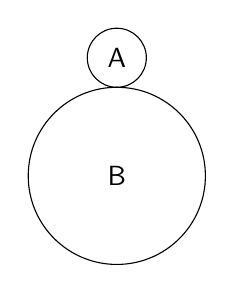
\begin{tikzpicture}[scale=.5]
    % Draw circle B (larger circle)
  \draw (0,0) circle (2.25cm);
    \node at (0,0) {B};
    
    % Draw circle A (smaller circle)
    \draw (0,3) circle (0.75cm);
    \node at (0,3) {A};
\end{tikzpicture}

\vspace{.5cm}

The radius of circle A is $\frac{1}{3}$ of the radius of circle B. Circle A rolls\\
around circle B one trip back to its starting point. How\\
many times will circle A revolve in total?

\vspace{.5cm}

\begin{tabular}{l@{\hspace{2em}}l@{\hspace{2em}}l@{\hspace{2em}}l@{\hspace{2em}}l}
  (a) $\frac{3}{2}$ & (b) 3 & (c) 6 & (d) $\frac{9}{2}$ & (e) 9
\end{tabular}
\end{center}

\vspace{.5cm}
\end{frame}

\begin{frame}{Animation of Coin Rotation Paradox}
  \hspace*{\dimexpr(\textwidth - .6\textwidth)/2\relax}
\begin{overlayarea}{\textwidth}{0.7\textheight}
\only<1>{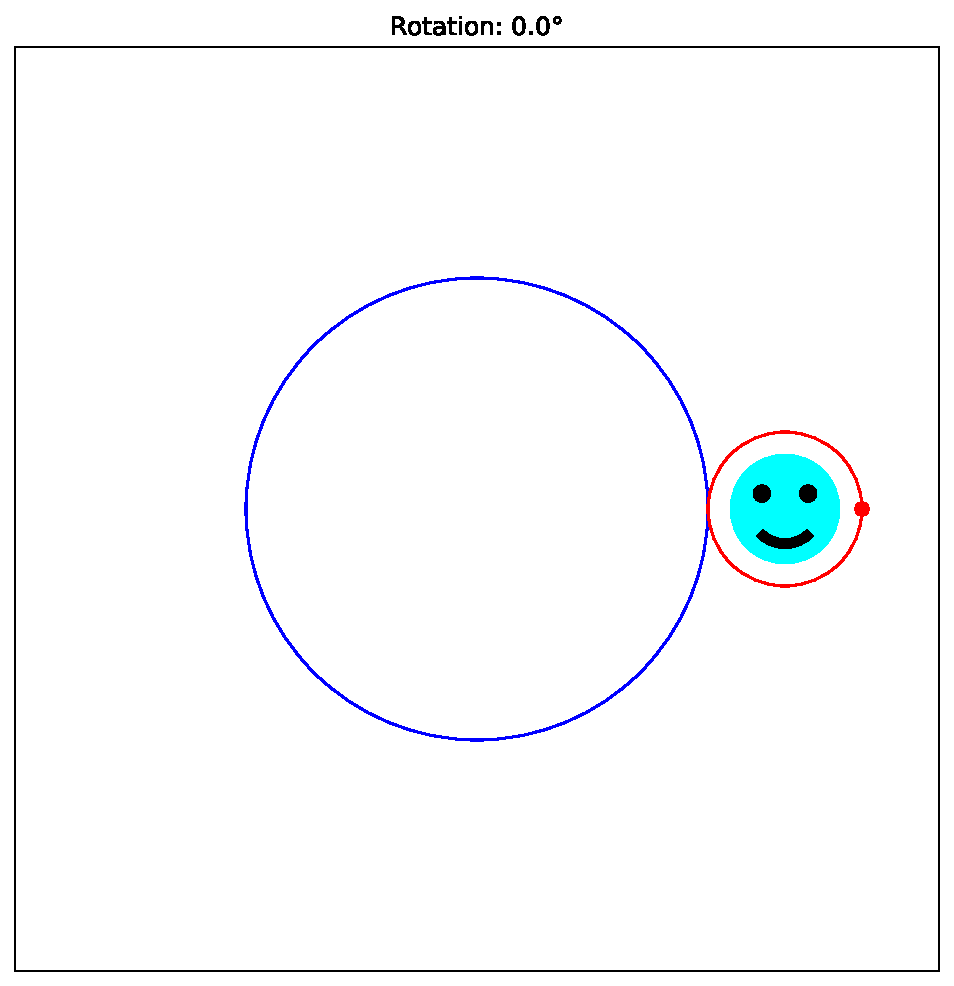
\includegraphics[width=.6\textwidth]{fig/note02/coin_rotation_0.pdf}\noindent}
\only<2>{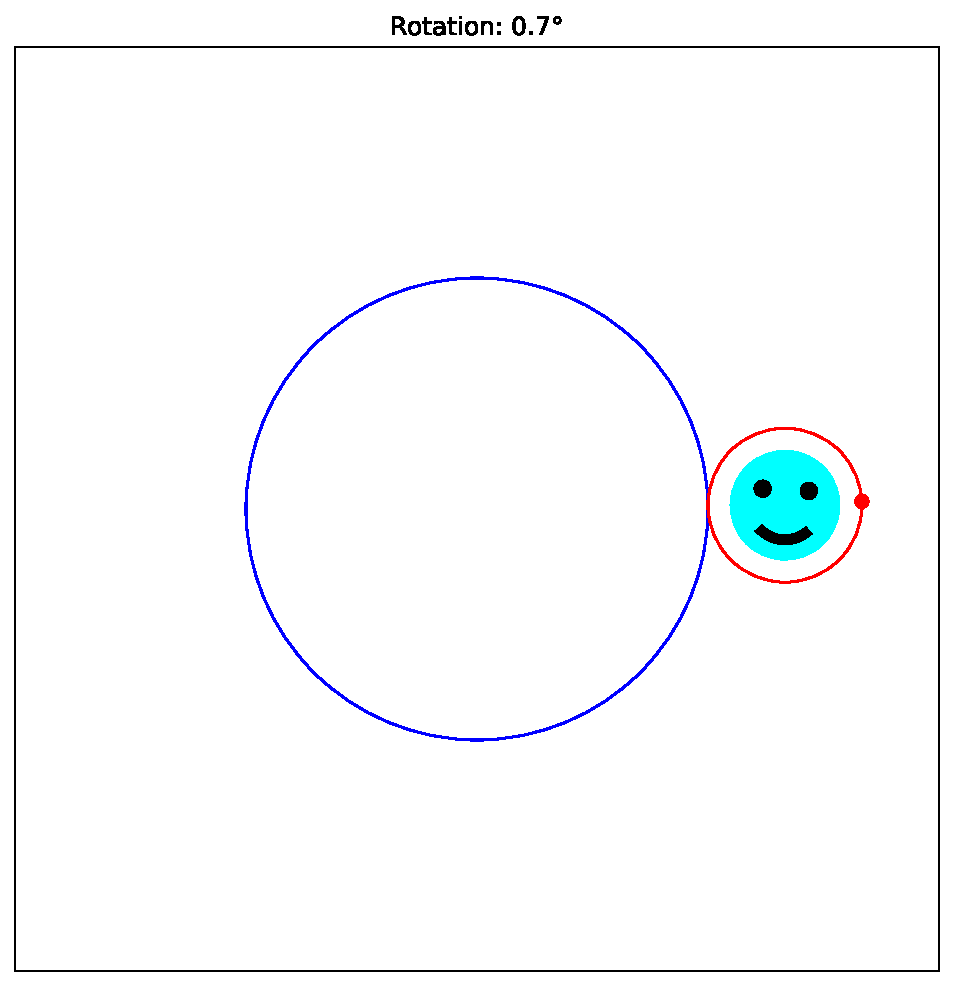
\includegraphics[width=.6\textwidth]{fig/note02/coin_rotation_1.pdf}\noindent}
\only<3>{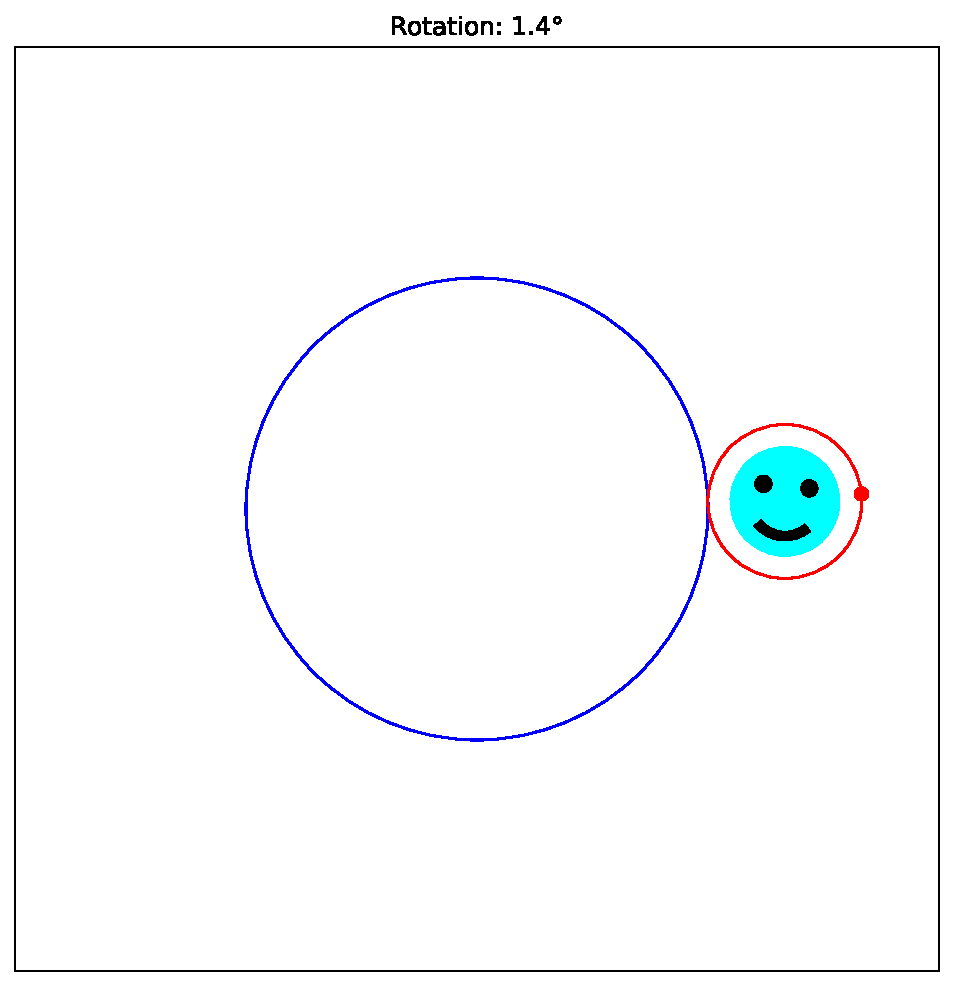
\includegraphics[width=.6\textwidth]{fig/note02/coin_rotation_2.pdf}\noindent}
\only<4>{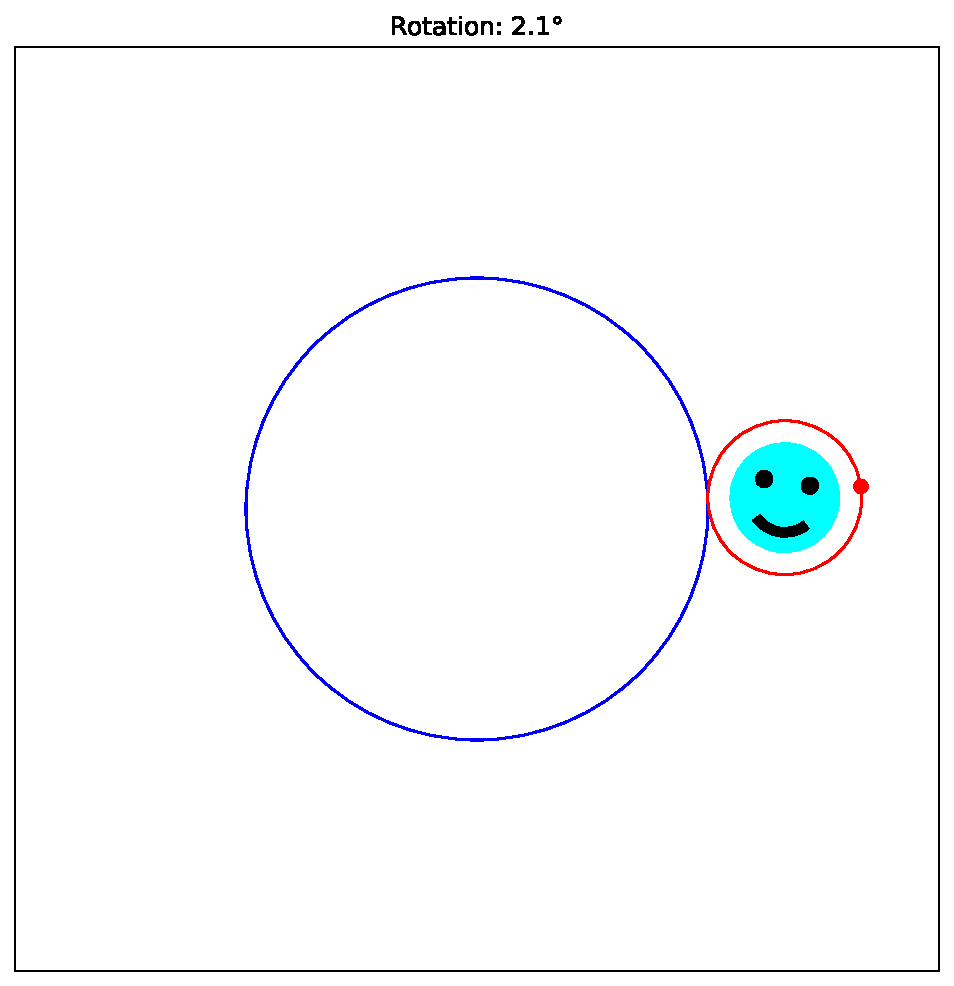
\includegraphics[width=.6\textwidth]{fig/note02/coin_rotation_3.pdf}\noindent}
\only<5>{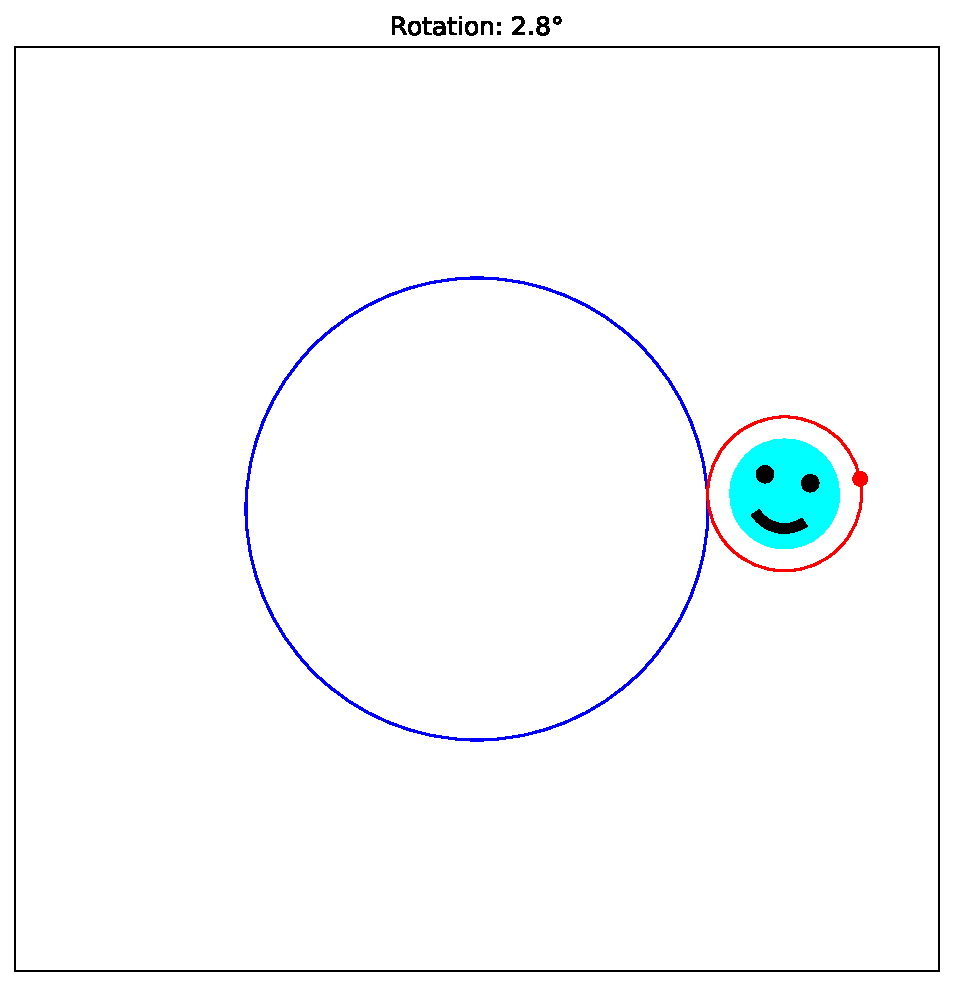
\includegraphics[width=.6\textwidth]{fig/note02/coin_rotation_4.pdf}\noindent}
\only<6>{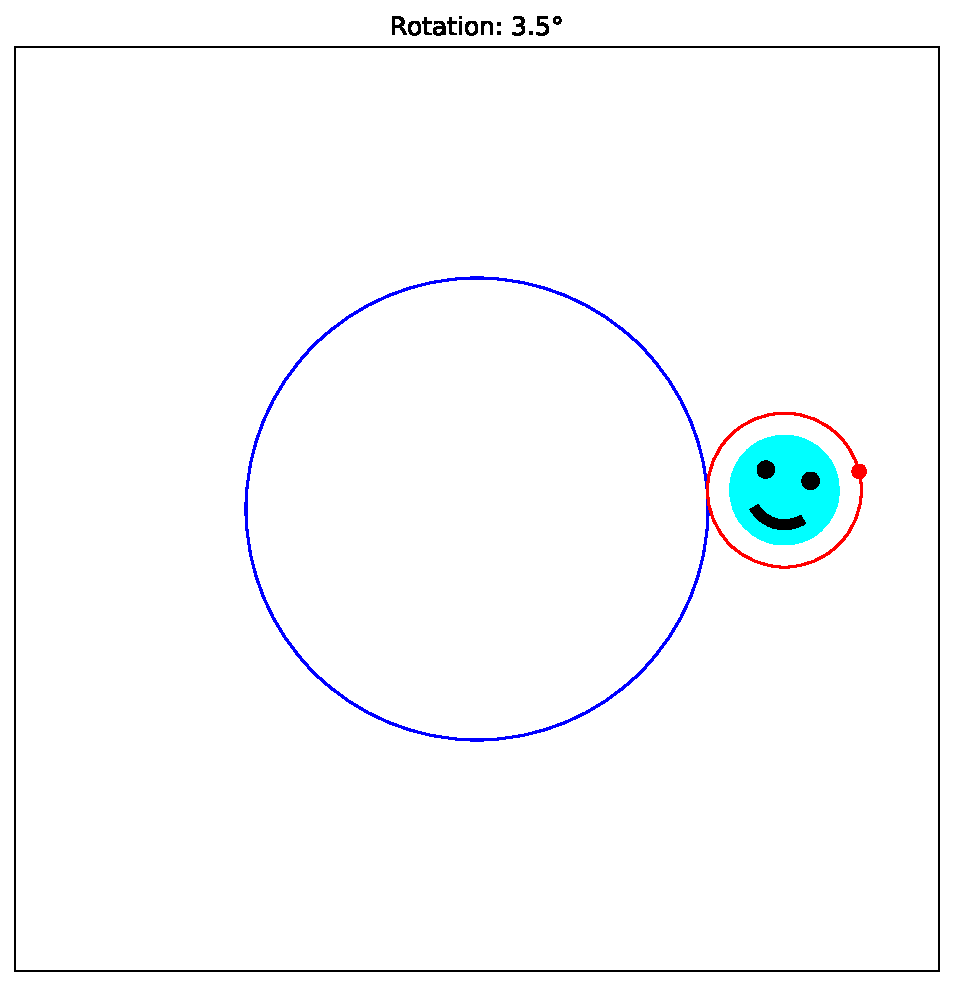
\includegraphics[width=.6\textwidth]{fig/note02/coin_rotation_5.pdf}\noindent}
\only<7>{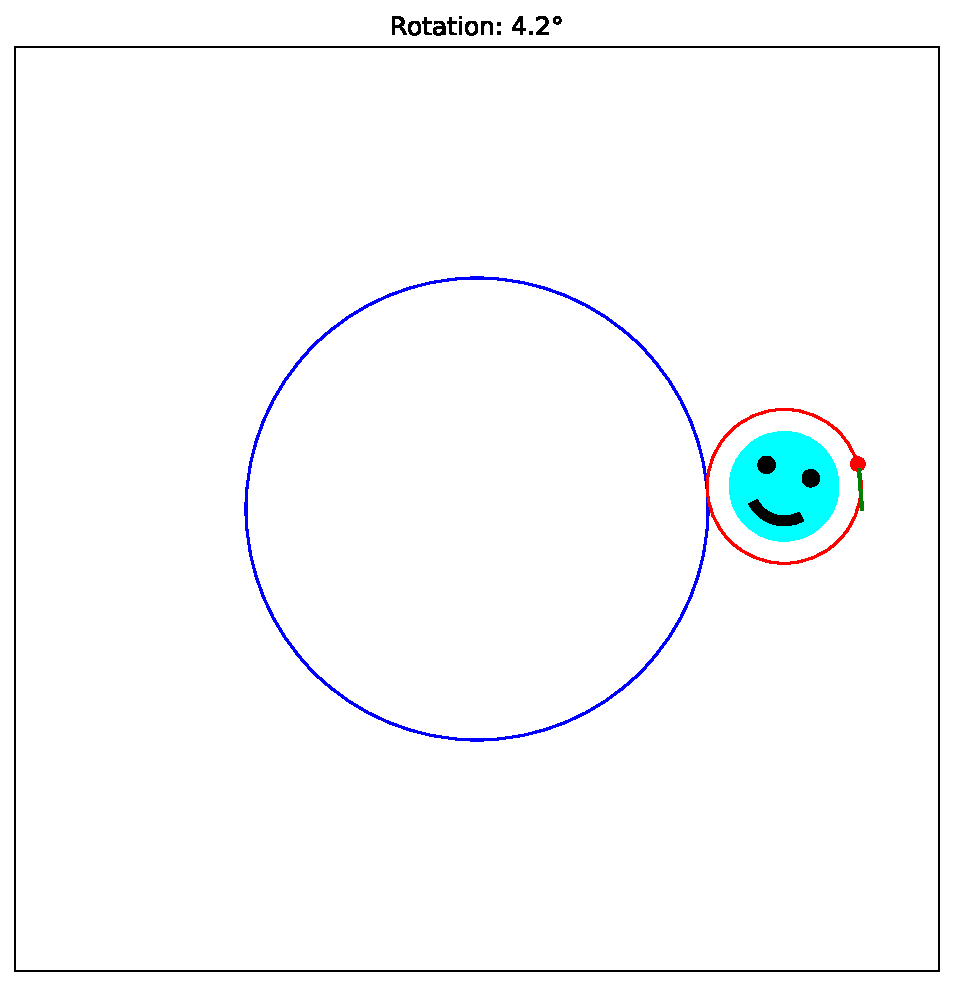
\includegraphics[width=.6\textwidth]{fig/note02/coin_rotation_6.pdf}\noindent}
\only<8>{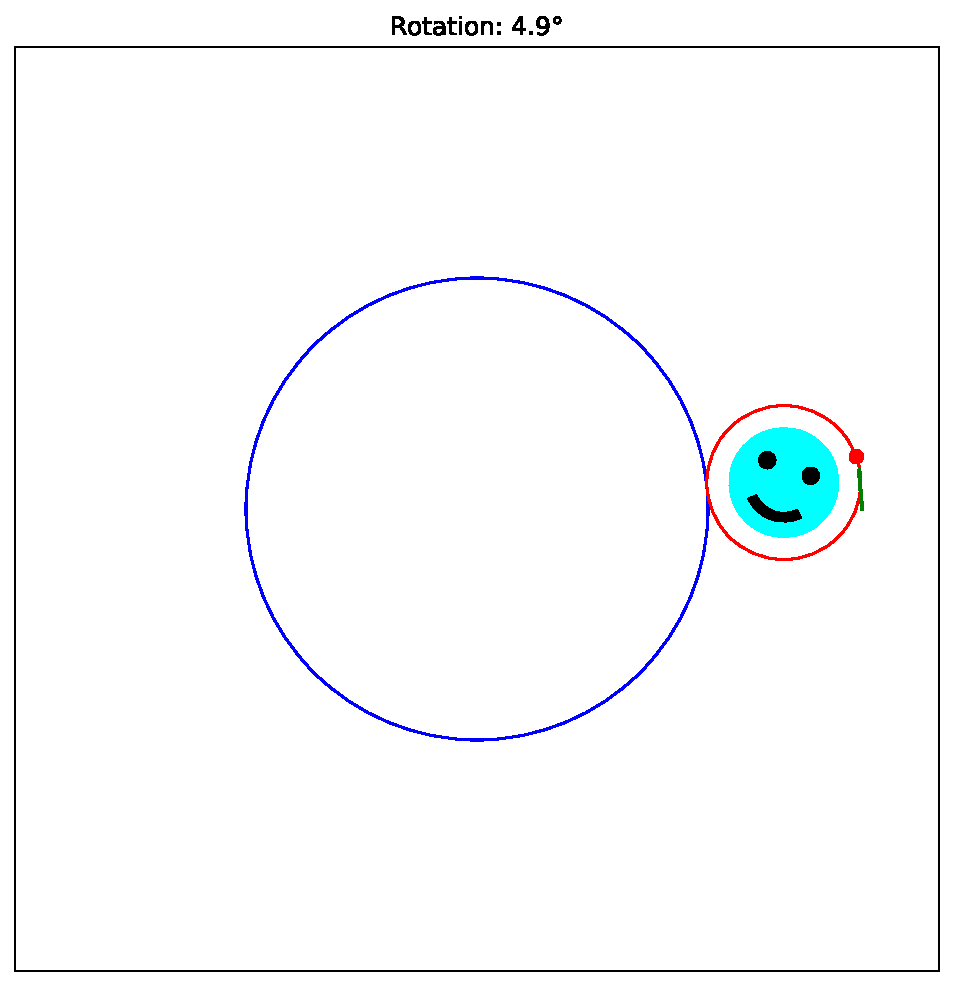
\includegraphics[width=.6\textwidth]{fig/note02/coin_rotation_7.pdf}\noindent}
\only<9>{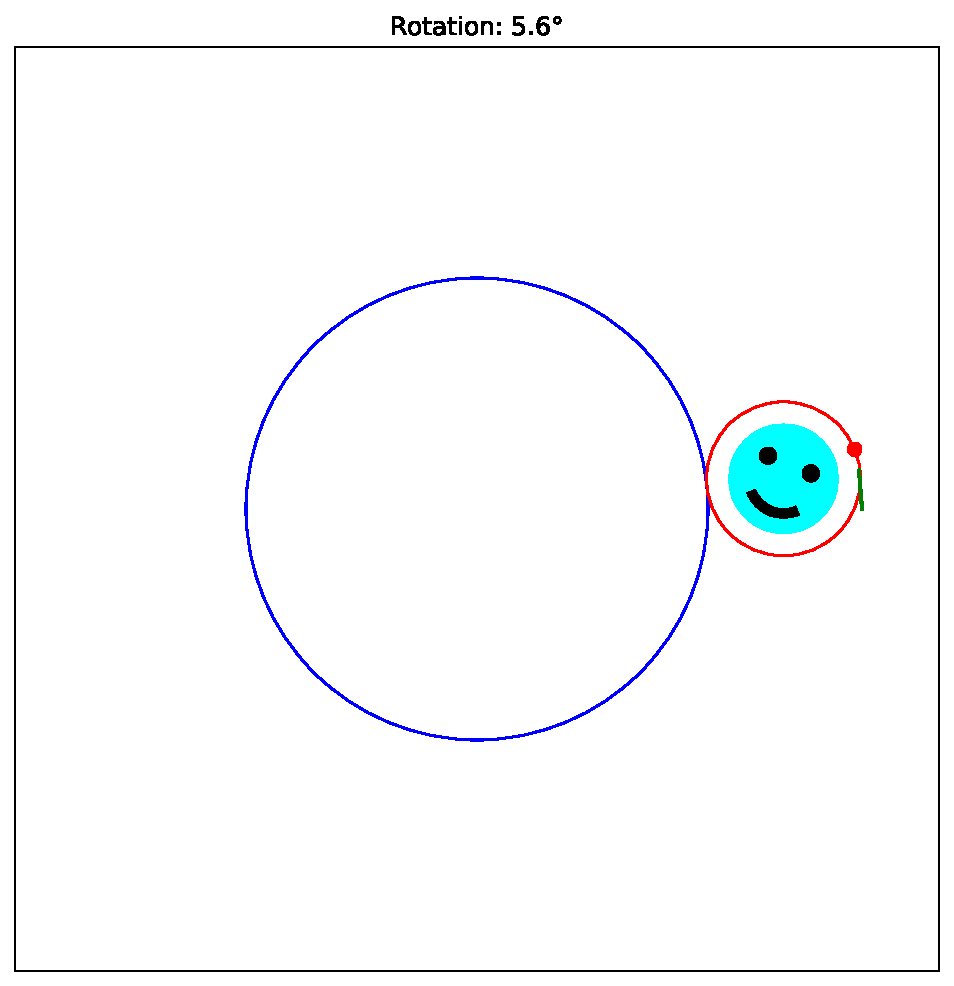
\includegraphics[width=.6\textwidth]{fig/note02/coin_rotation_8.pdf}\noindent}
\only<10>{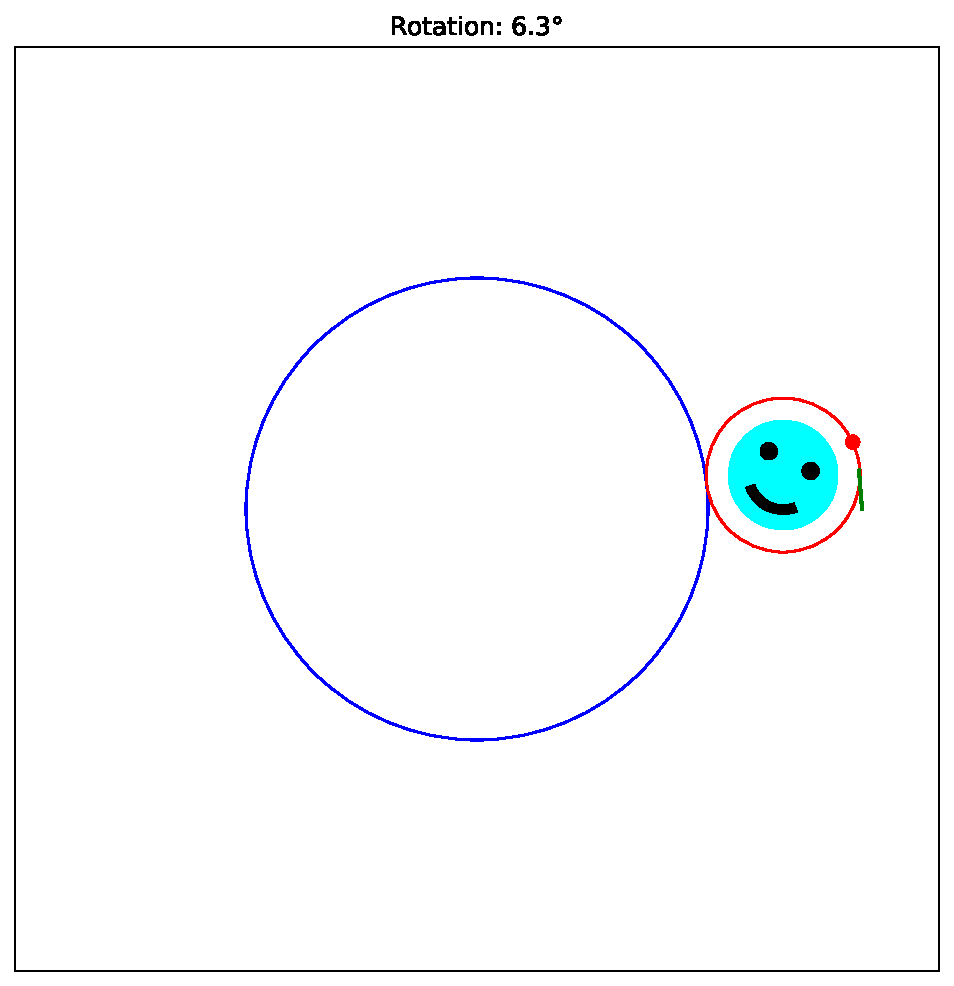
\includegraphics[width=.6\textwidth]{fig/note02/coin_rotation_9.pdf}\noindent}
\only<11>{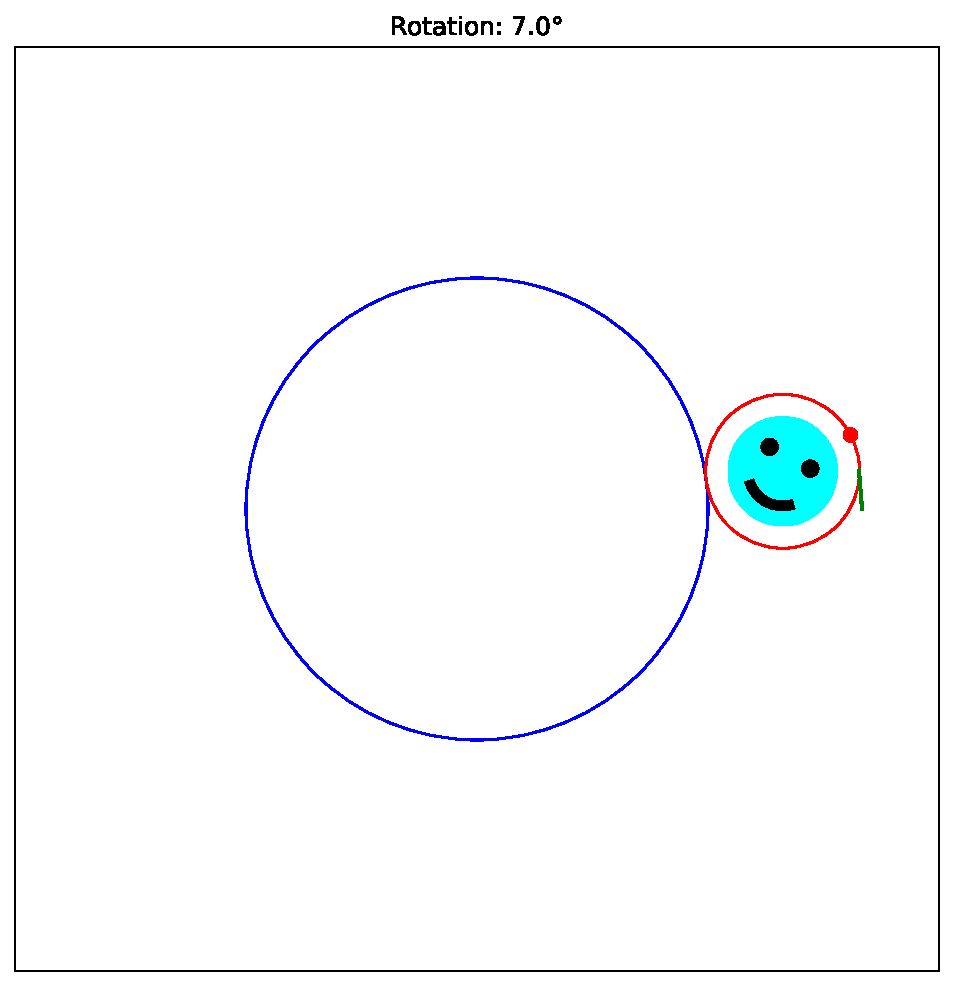
\includegraphics[width=.6\textwidth]{fig/note02/coin_rotation_10.pdf}\noindent}
\only<12>{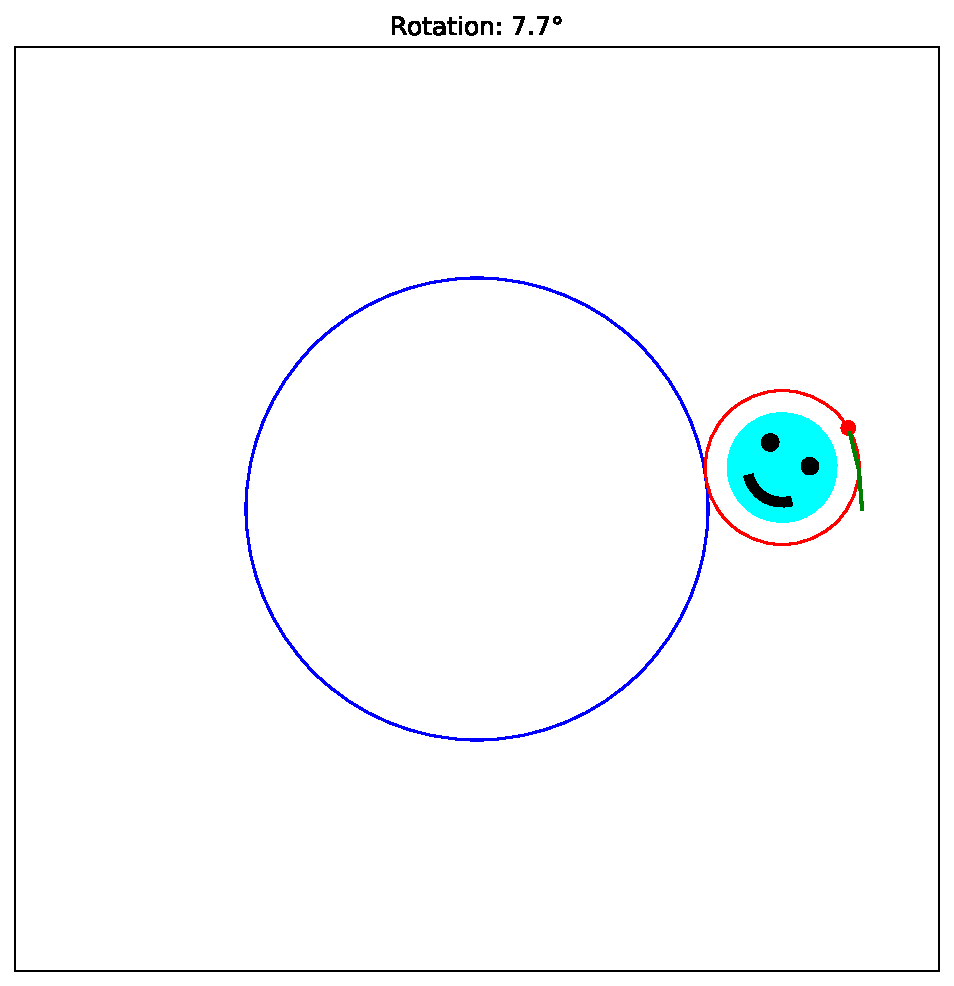
\includegraphics[width=.6\textwidth]{fig/note02/coin_rotation_11.pdf}\noindent}
\only<13>{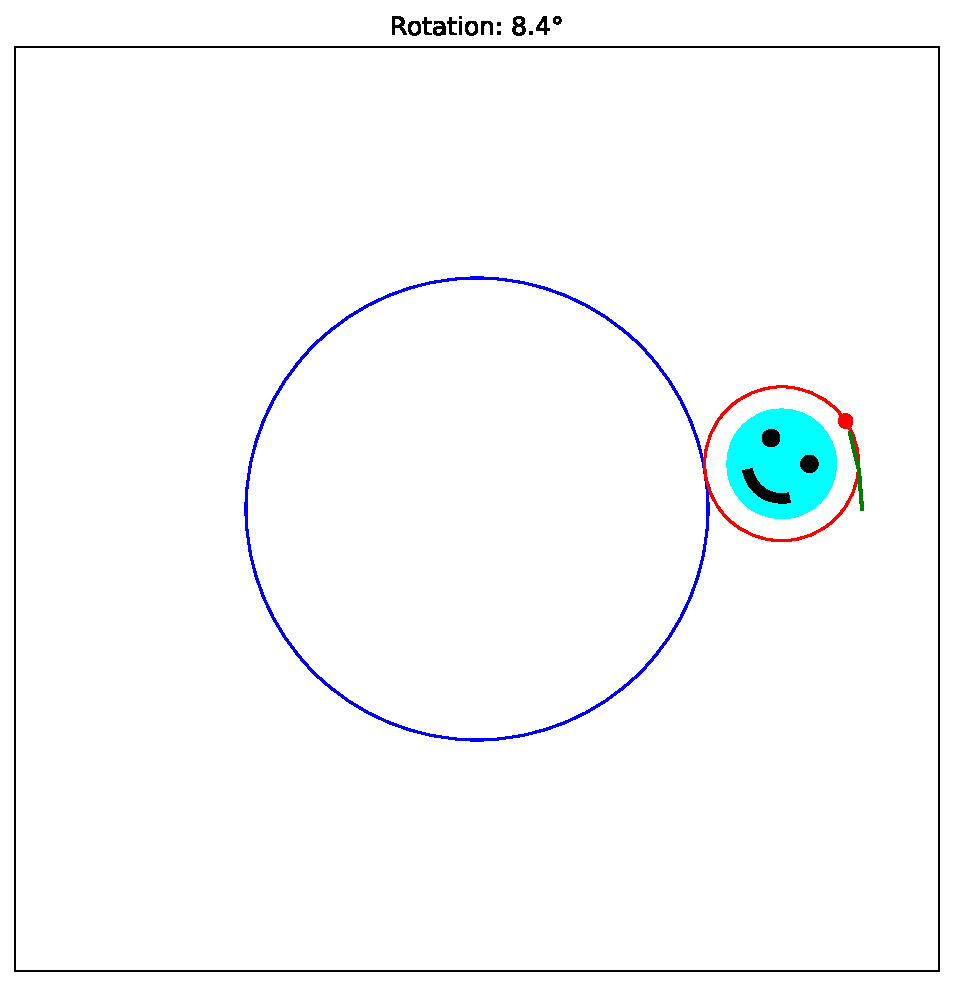
\includegraphics[width=.6\textwidth]{fig/note02/coin_rotation_12.pdf}\noindent}
\only<14>{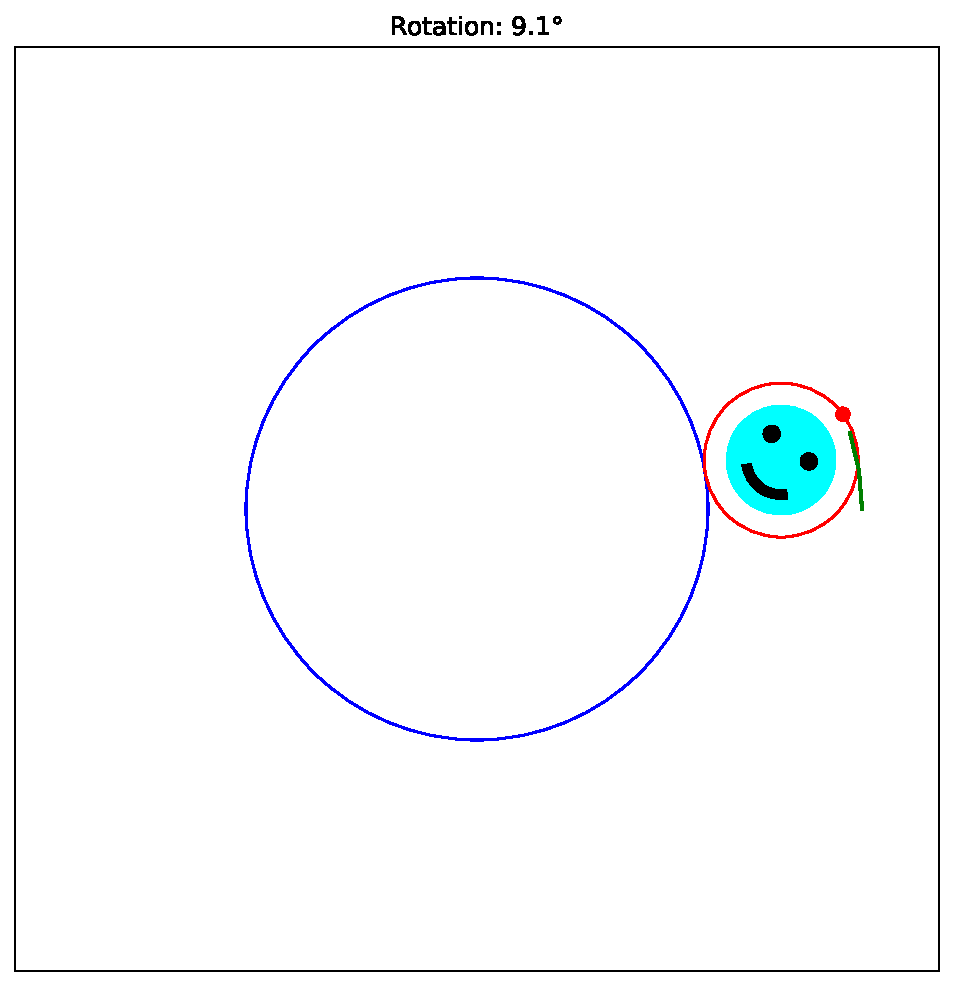
\includegraphics[width=.6\textwidth]{fig/note02/coin_rotation_13.pdf}\noindent}
\only<15>{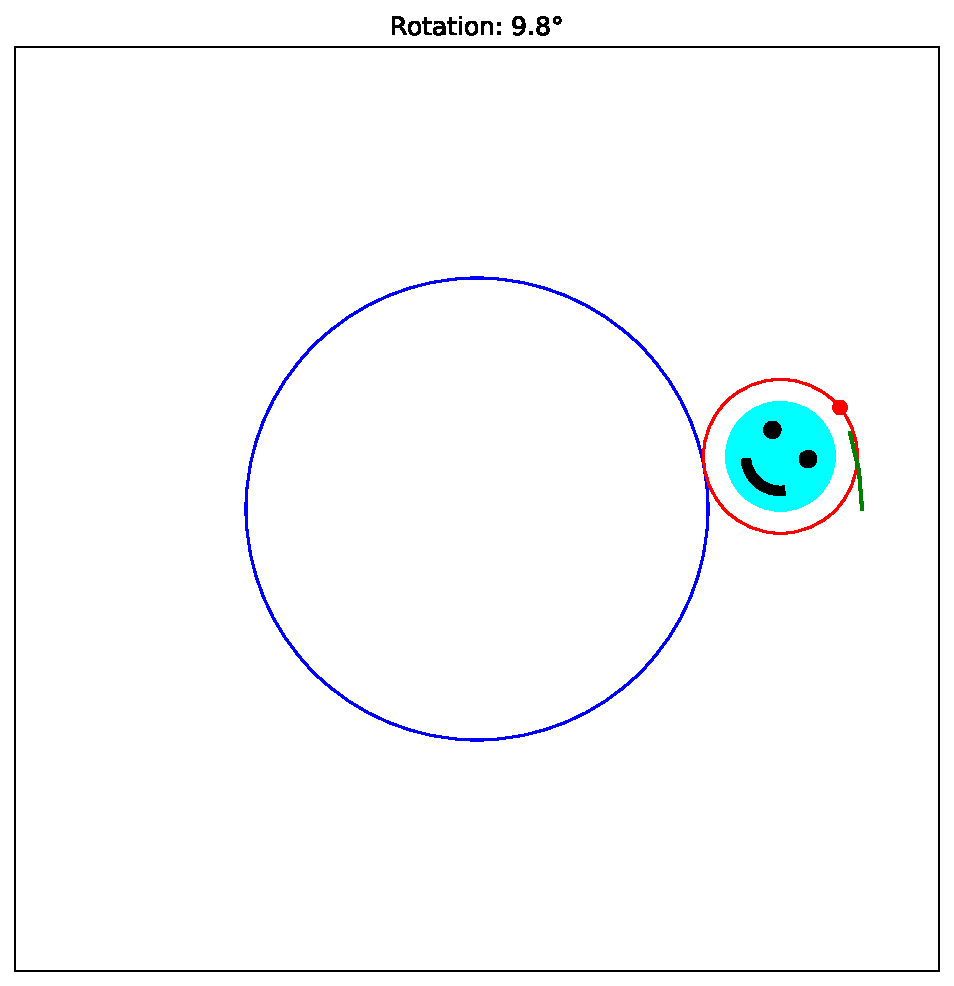
\includegraphics[width=.6\textwidth]{fig/note02/coin_rotation_14.pdf}\noindent}
\only<16>{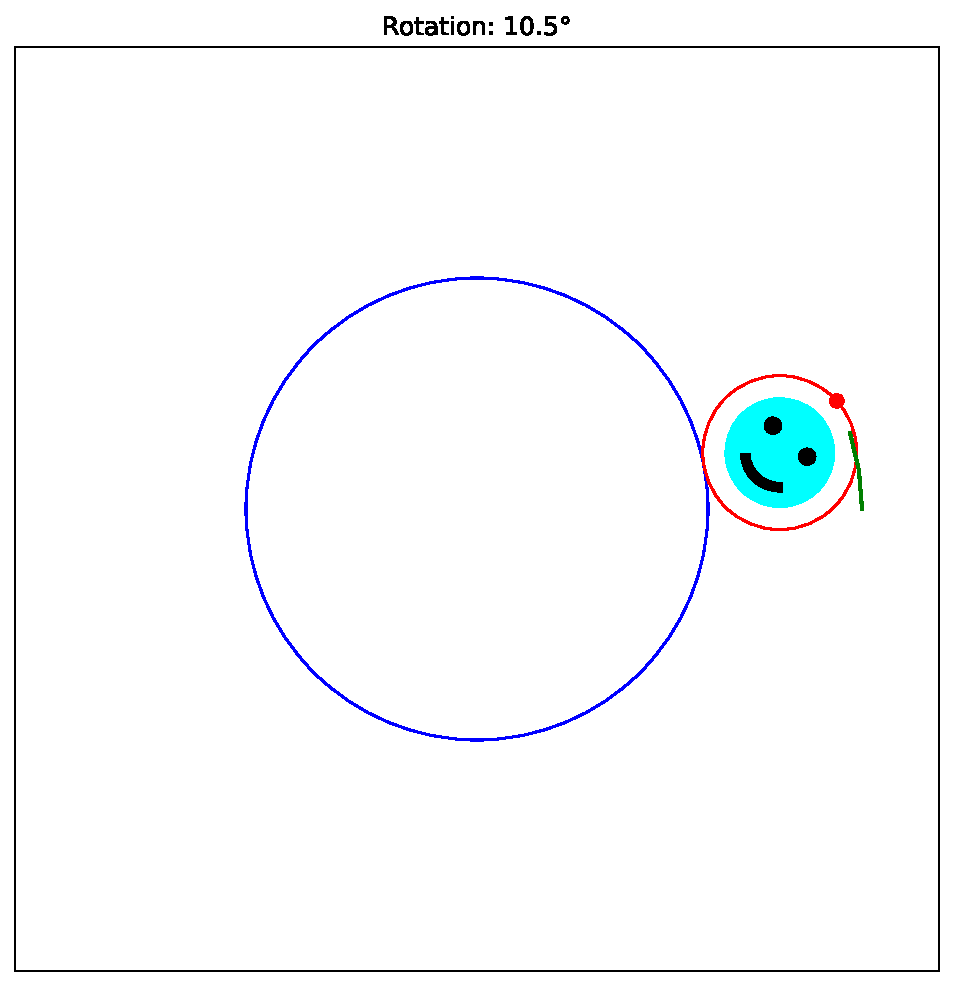
\includegraphics[width=.6\textwidth]{fig/note02/coin_rotation_15.pdf}\noindent}
\only<17>{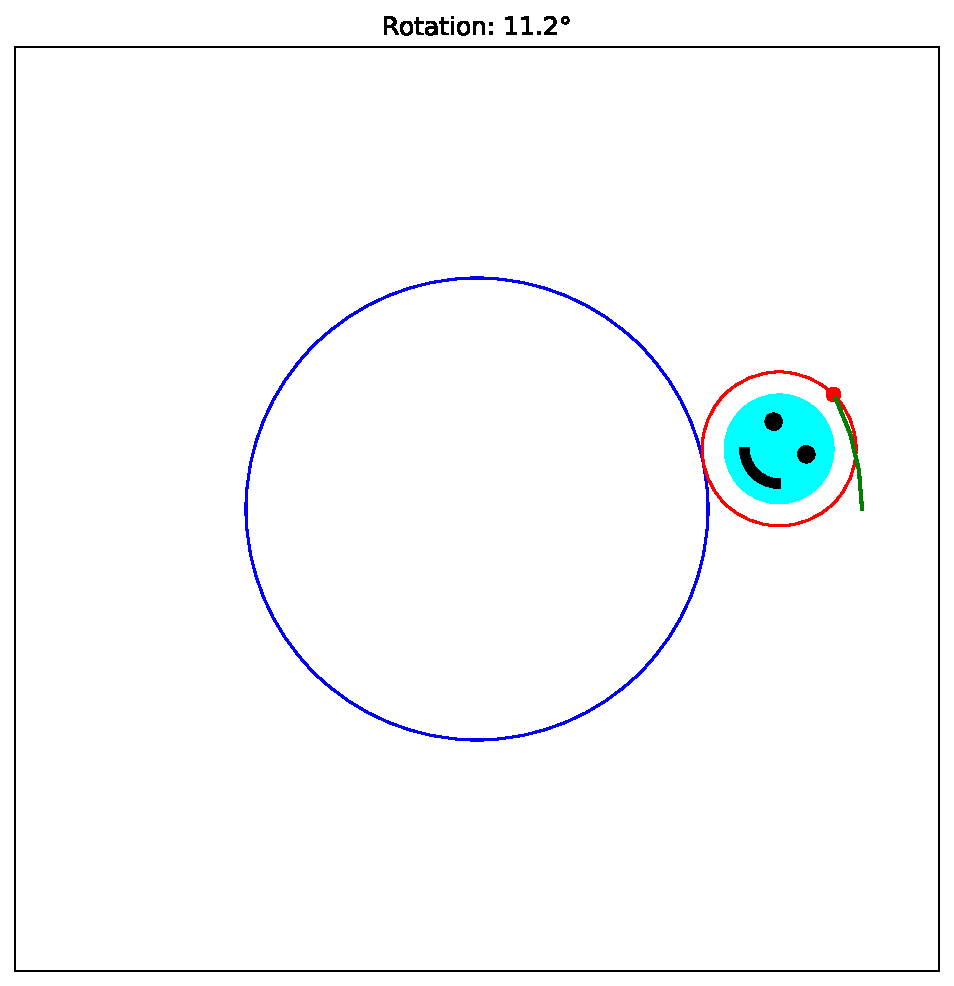
\includegraphics[width=.6\textwidth]{fig/note02/coin_rotation_16.pdf}\noindent}
\only<18>{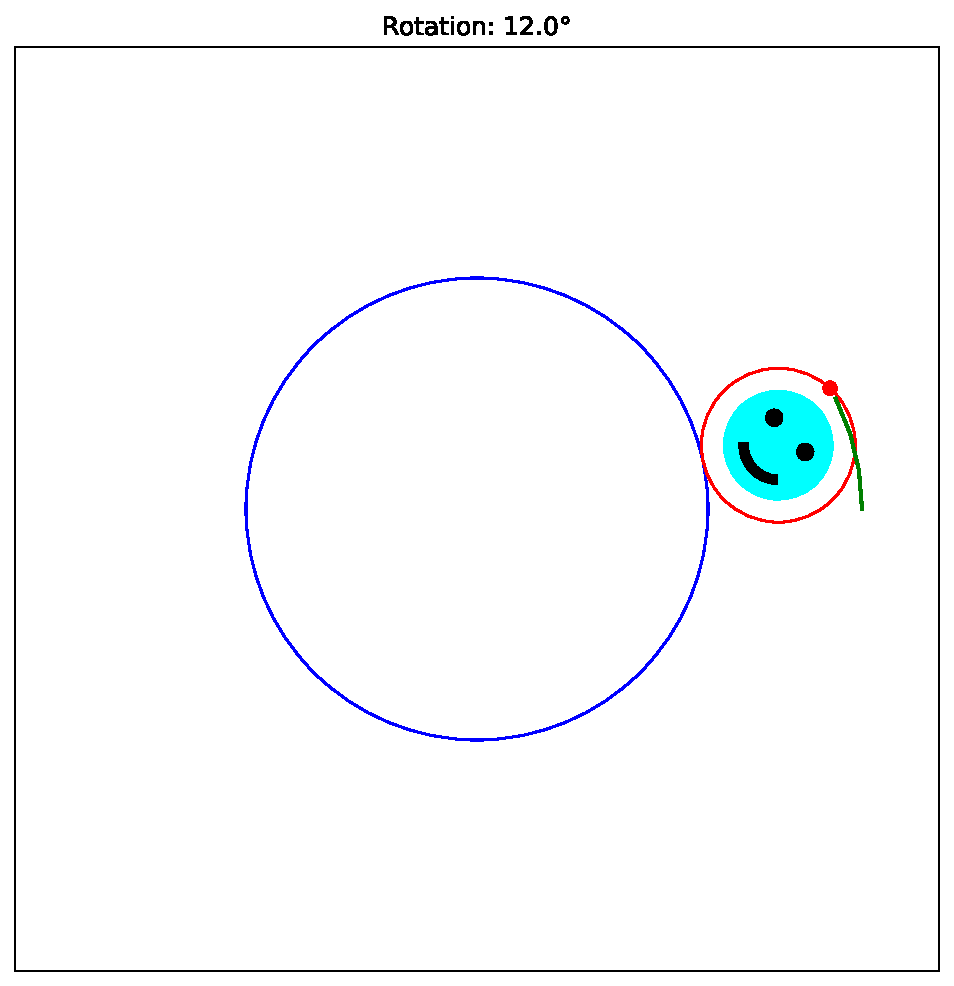
\includegraphics[width=.6\textwidth]{fig/note02/coin_rotation_17.pdf}\noindent}
\only<19>{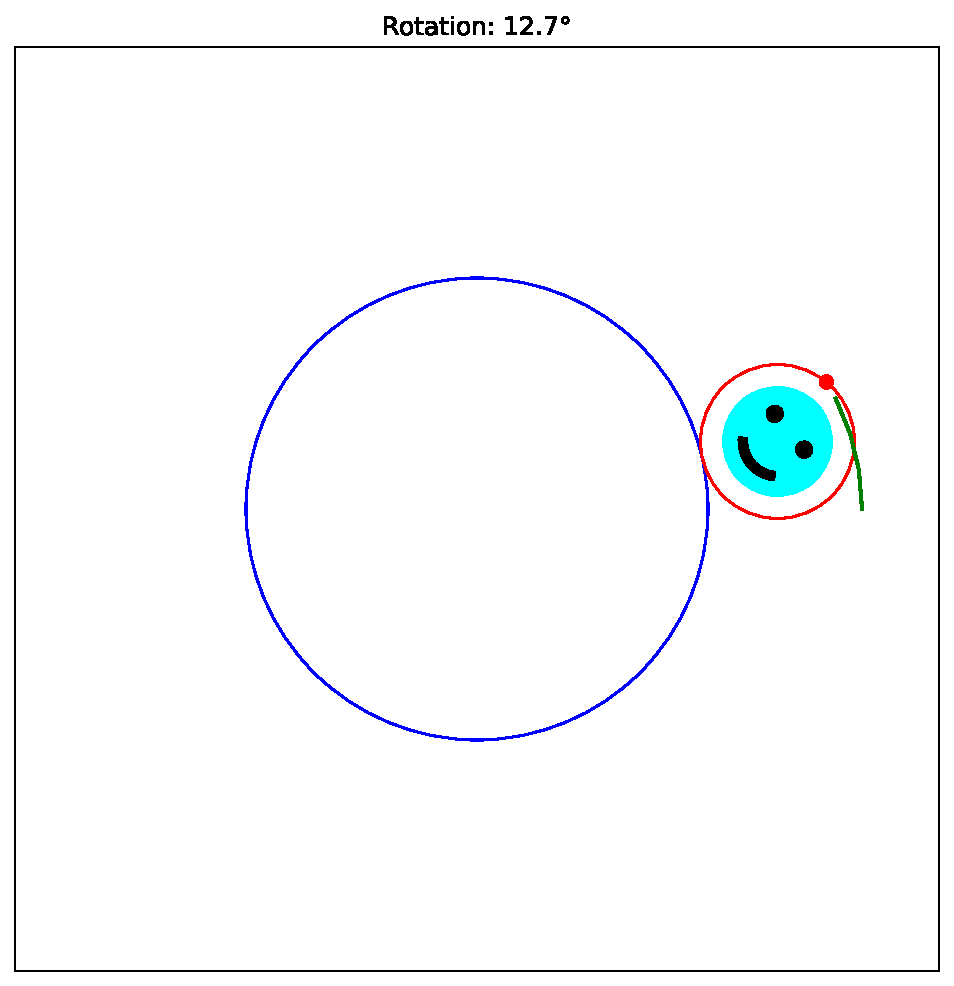
\includegraphics[width=.6\textwidth]{fig/note02/coin_rotation_18.pdf}\noindent}
\only<20>{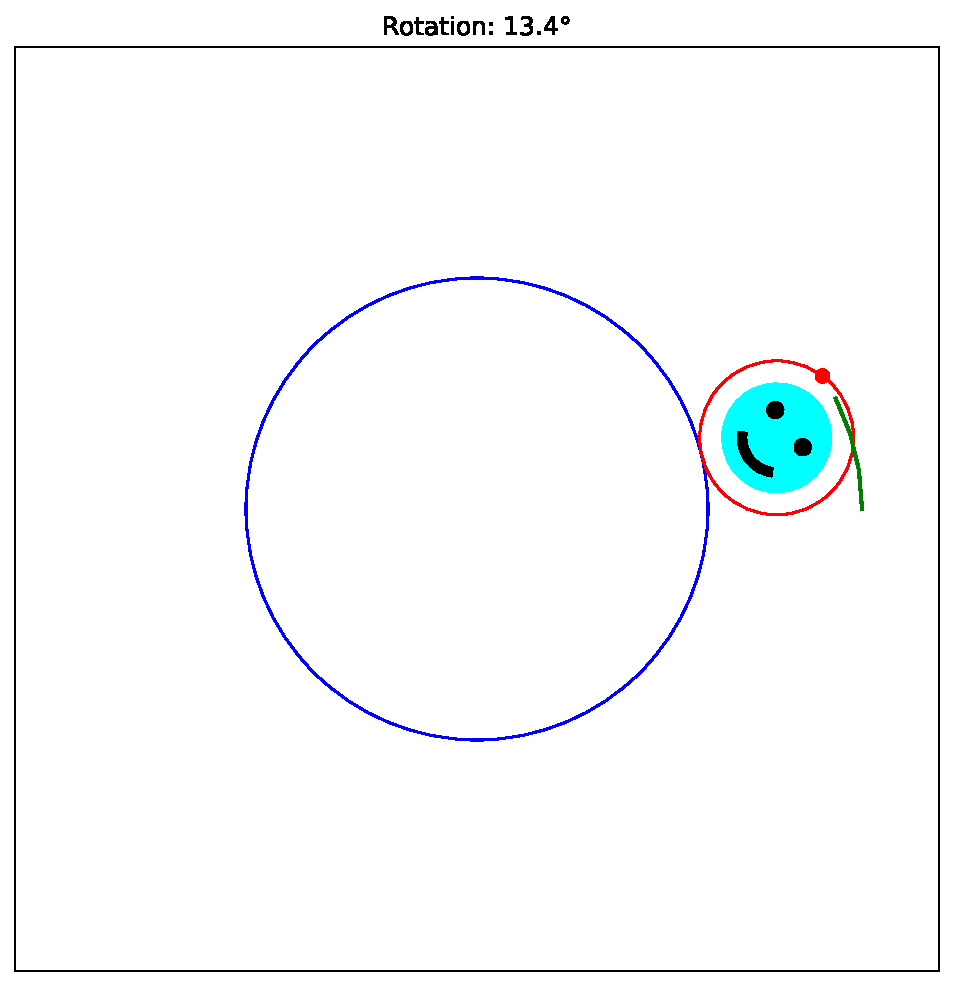
\includegraphics[width=.6\textwidth]{fig/note02/coin_rotation_19.pdf}\noindent}
\only<21>{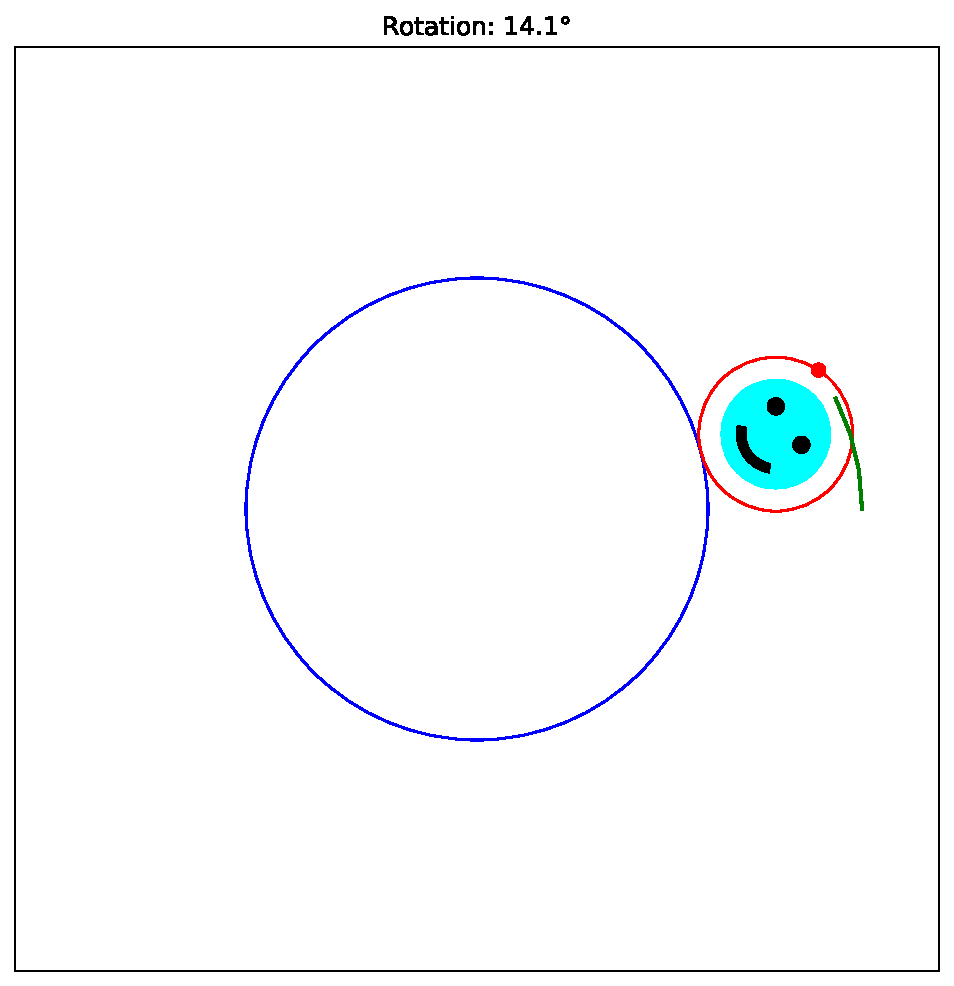
\includegraphics[width=.6\textwidth]{fig/note02/coin_rotation_20.pdf}\noindent}
\only<22>{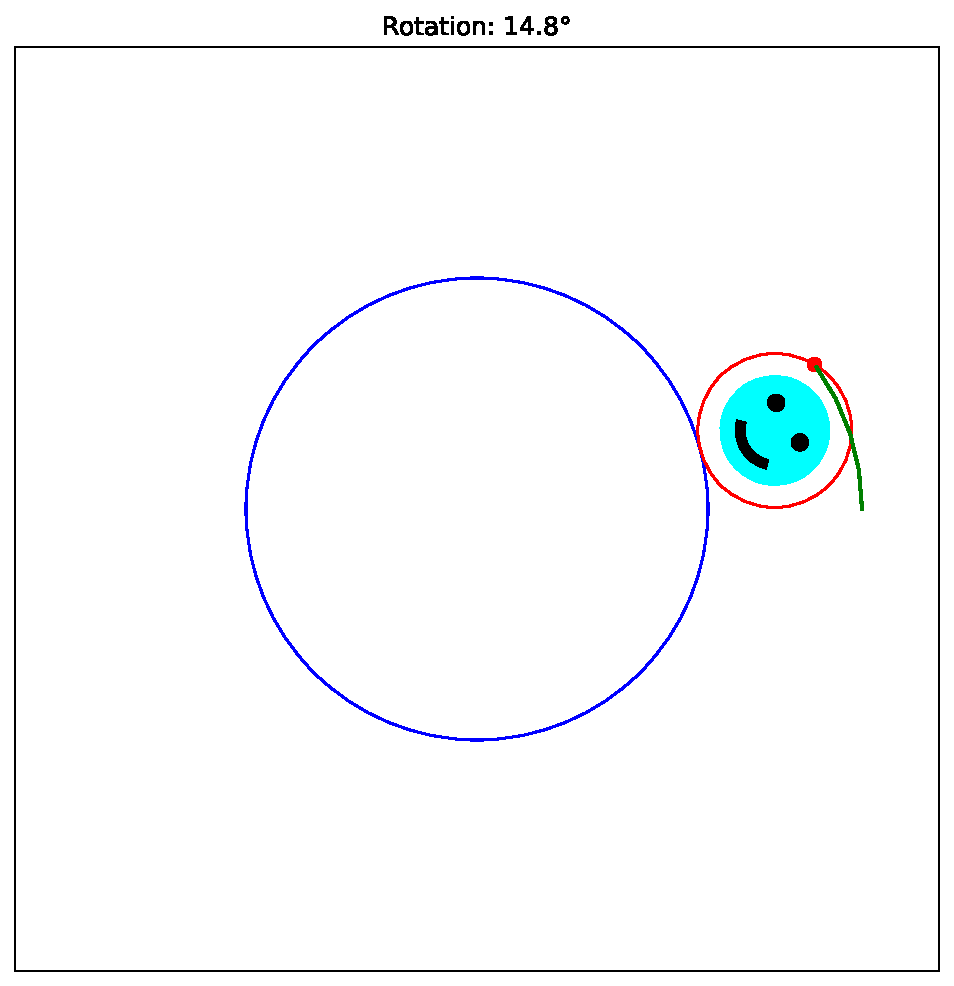
\includegraphics[width=.6\textwidth]{fig/note02/coin_rotation_21.pdf}\noindent}
\only<23>{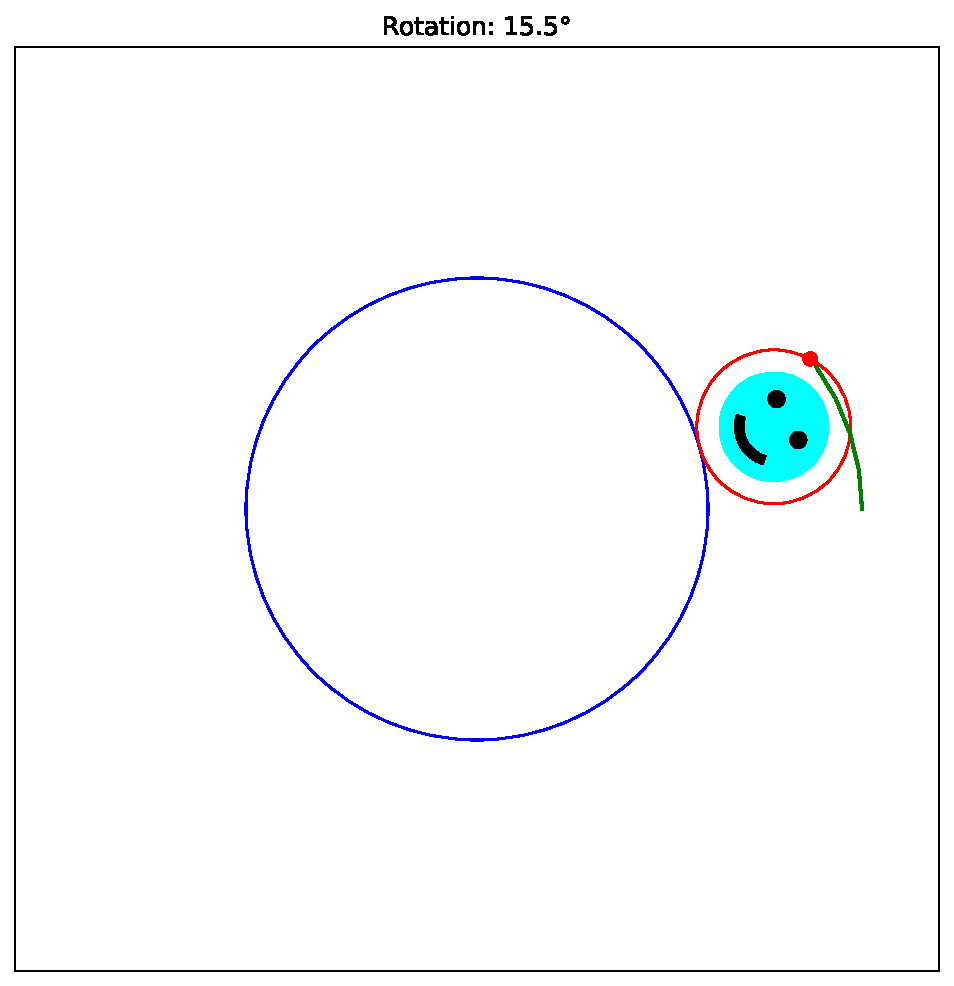
\includegraphics[width=.6\textwidth]{fig/note02/coin_rotation_22.pdf}\noindent}
\only<24>{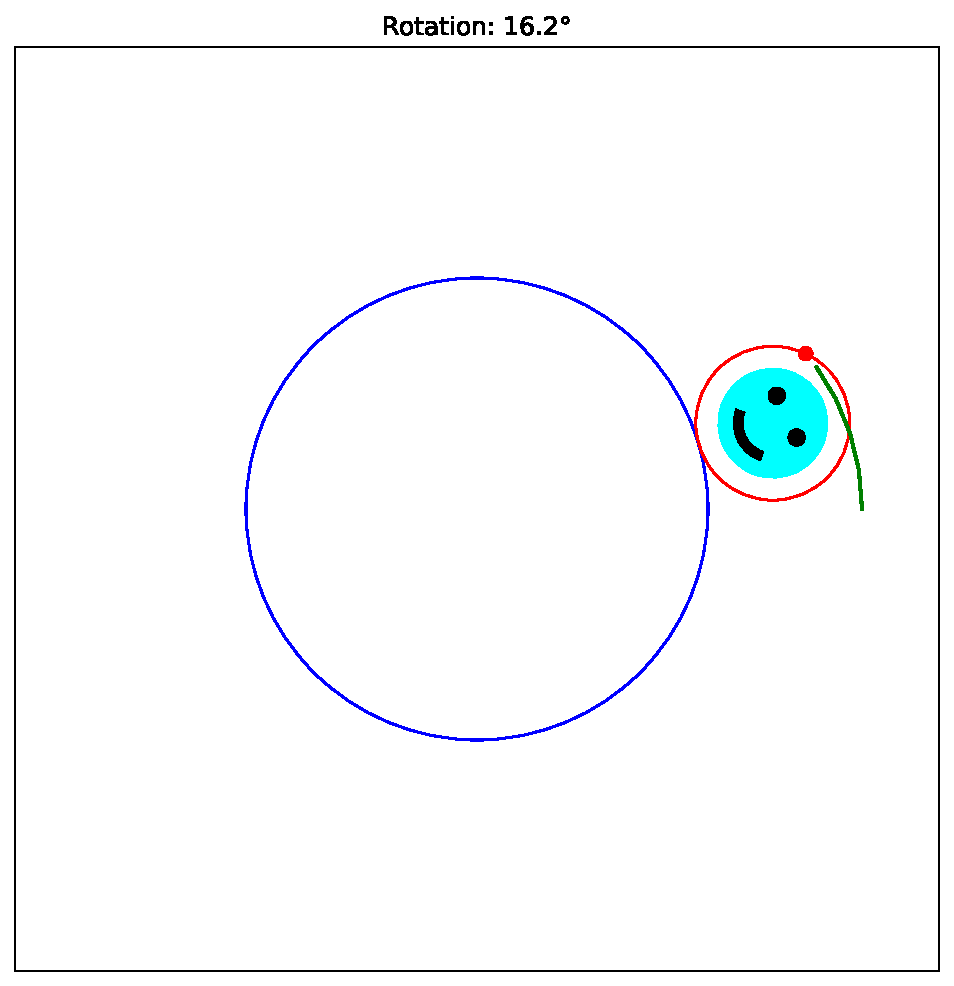
\includegraphics[width=.6\textwidth]{fig/note02/coin_rotation_23.pdf}\noindent}
\only<25>{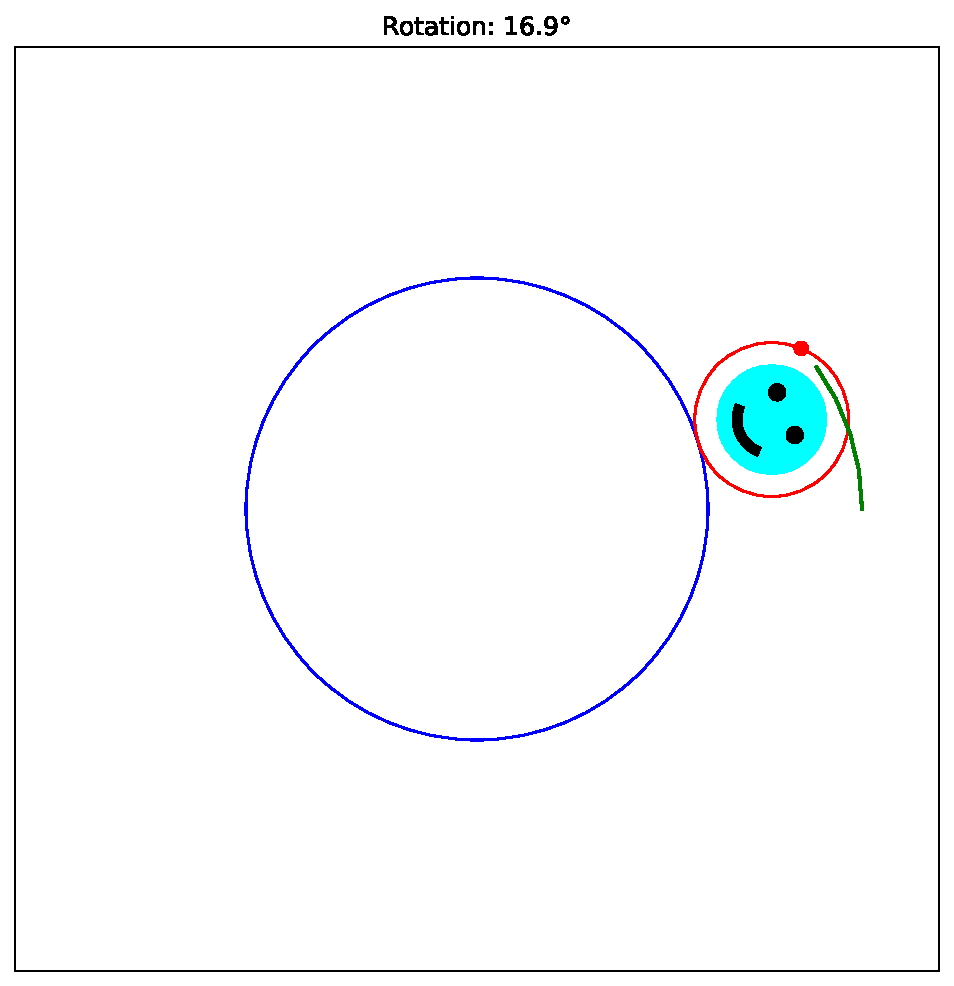
\includegraphics[width=.6\textwidth]{fig/note02/coin_rotation_24.pdf}\noindent}
\only<26>{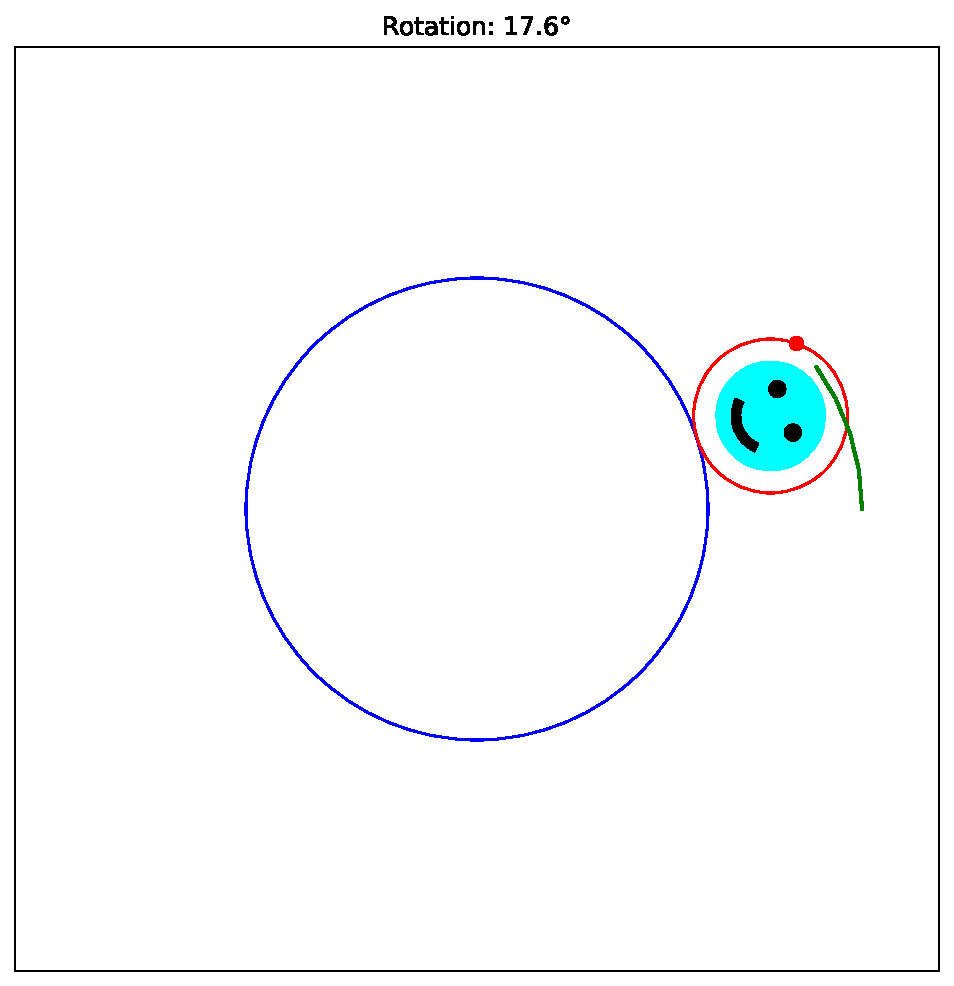
\includegraphics[width=.6\textwidth]{fig/note02/coin_rotation_25.pdf}\noindent}
\only<27>{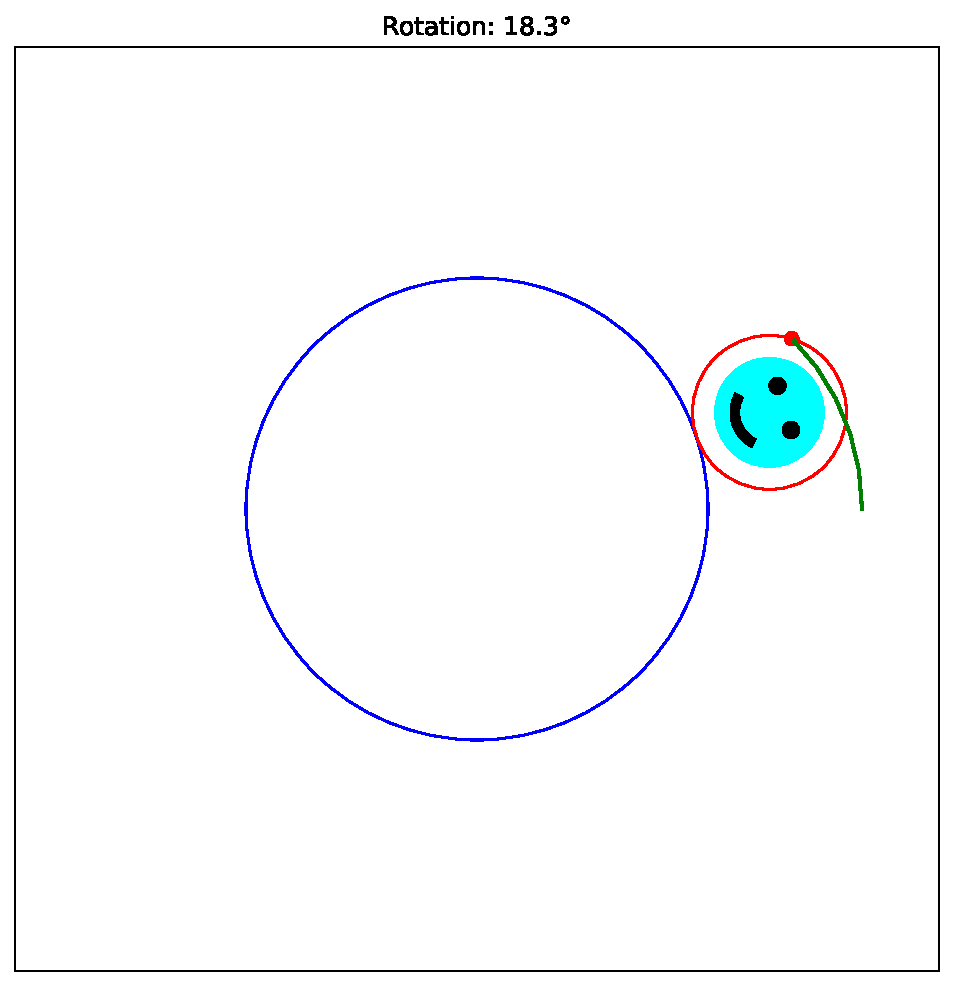
\includegraphics[width=.6\textwidth]{fig/note02/coin_rotation_26.pdf}\noindent}
\only<28>{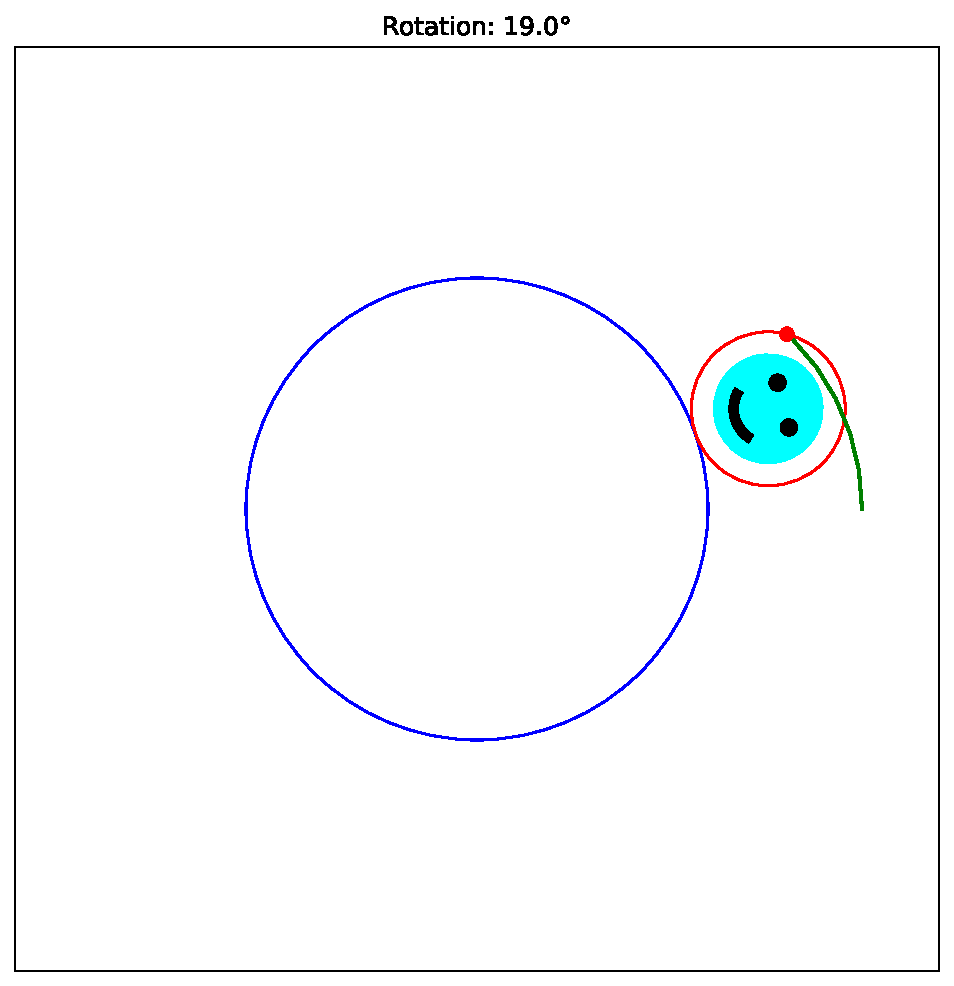
\includegraphics[width=.6\textwidth]{fig/note02/coin_rotation_27.pdf}\noindent}
\only<29>{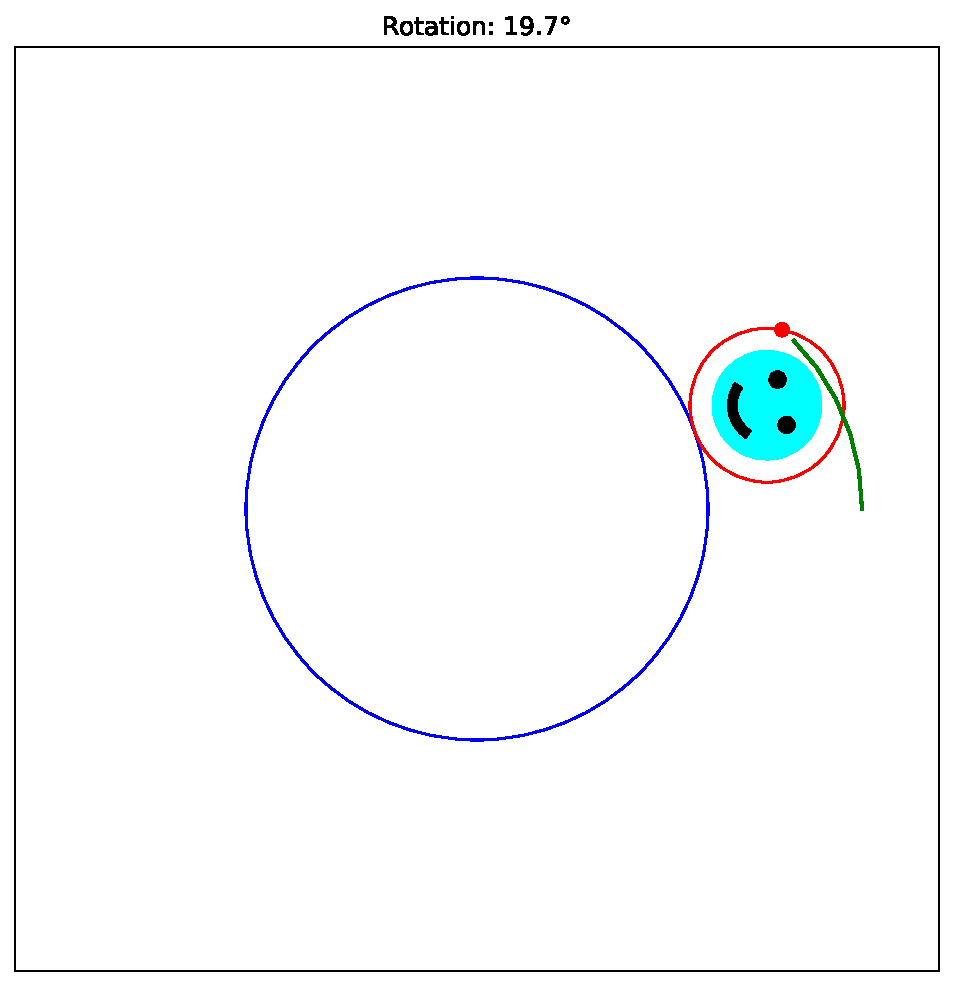
\includegraphics[width=.6\textwidth]{fig/note02/coin_rotation_28.pdf}\noindent}
\only<30>{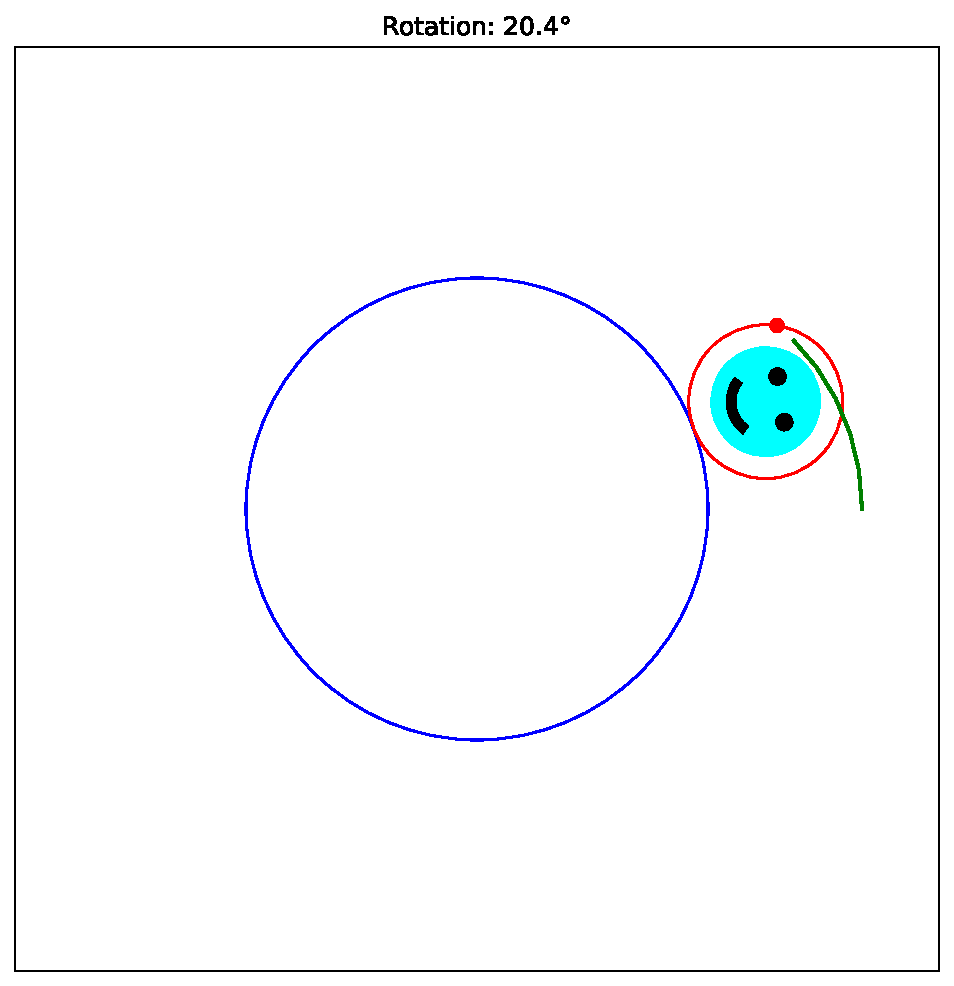
\includegraphics[width=.6\textwidth]{fig/note02/coin_rotation_29.pdf}\noindent}
\only<31>{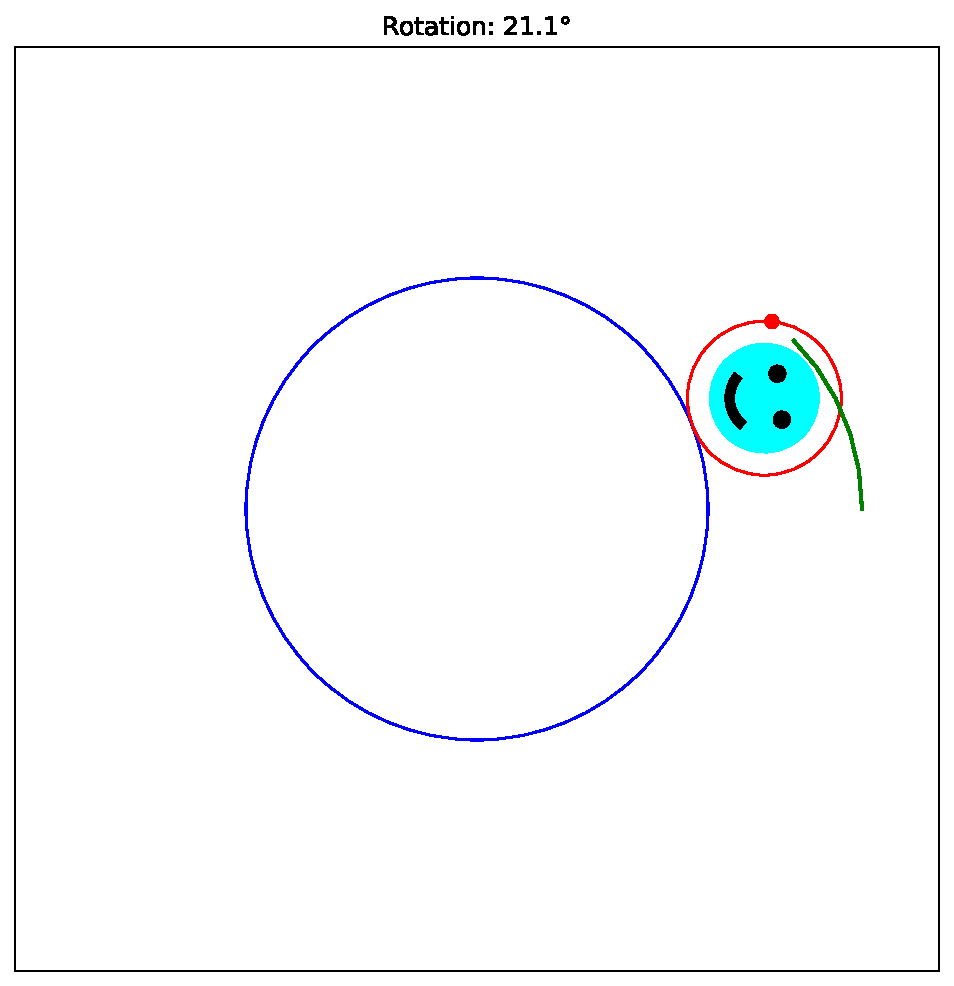
\includegraphics[width=.6\textwidth]{fig/note02/coin_rotation_30.pdf}\noindent}
\only<32>{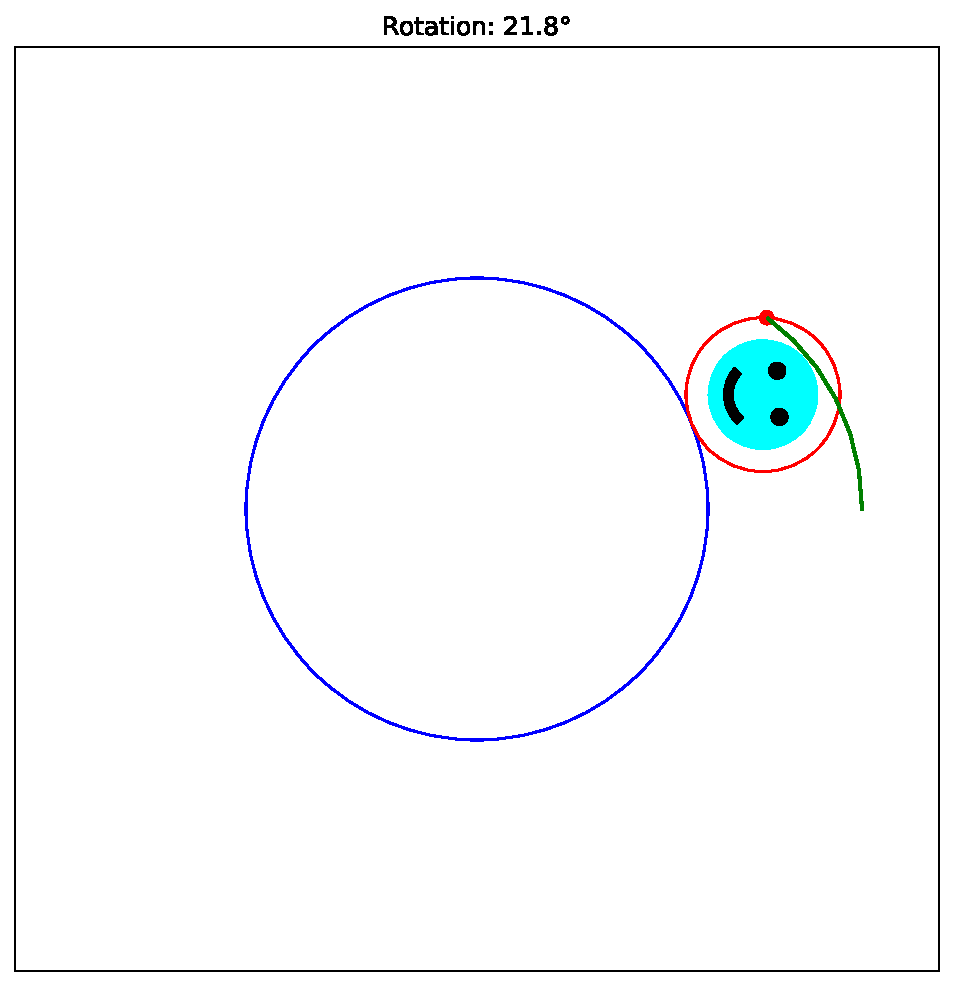
\includegraphics[width=.6\textwidth]{fig/note02/coin_rotation_31.pdf}\noindent}
\only<33>{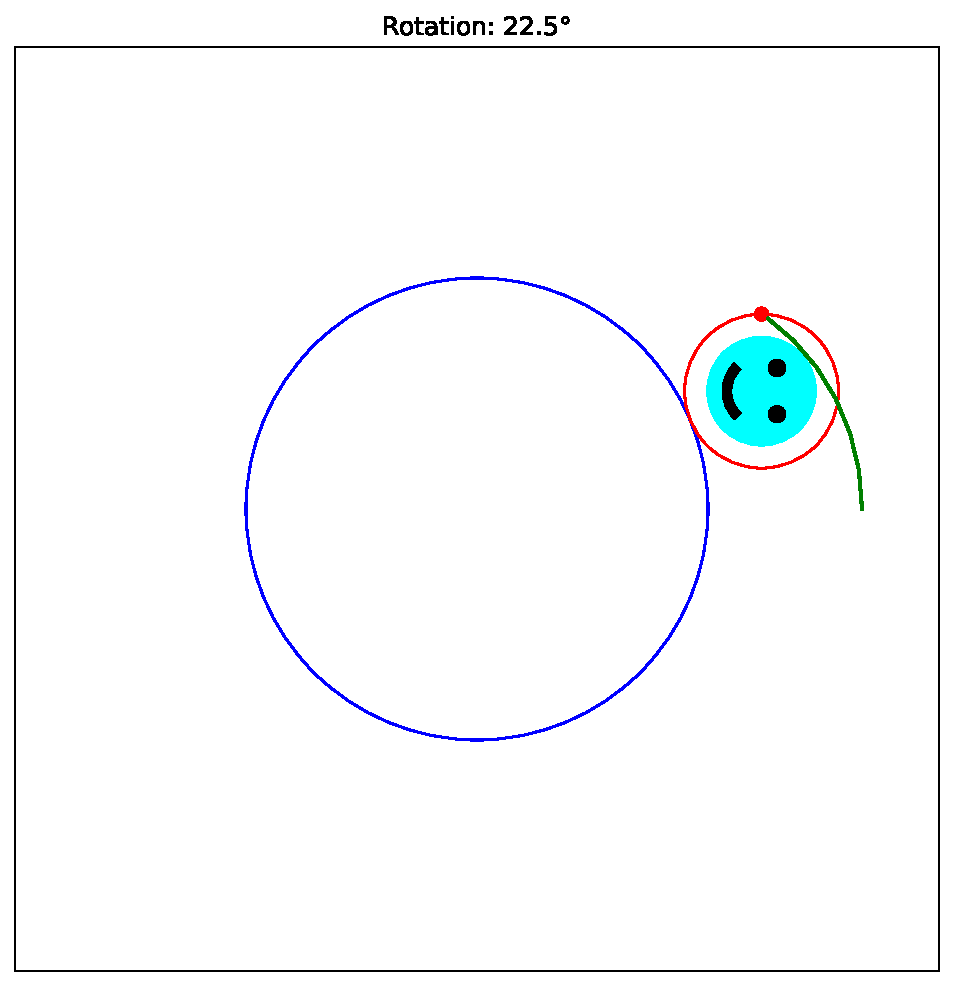
\includegraphics[width=.6\textwidth]{fig/note02/coin_rotation_32.pdf}\noindent}
\only<34>{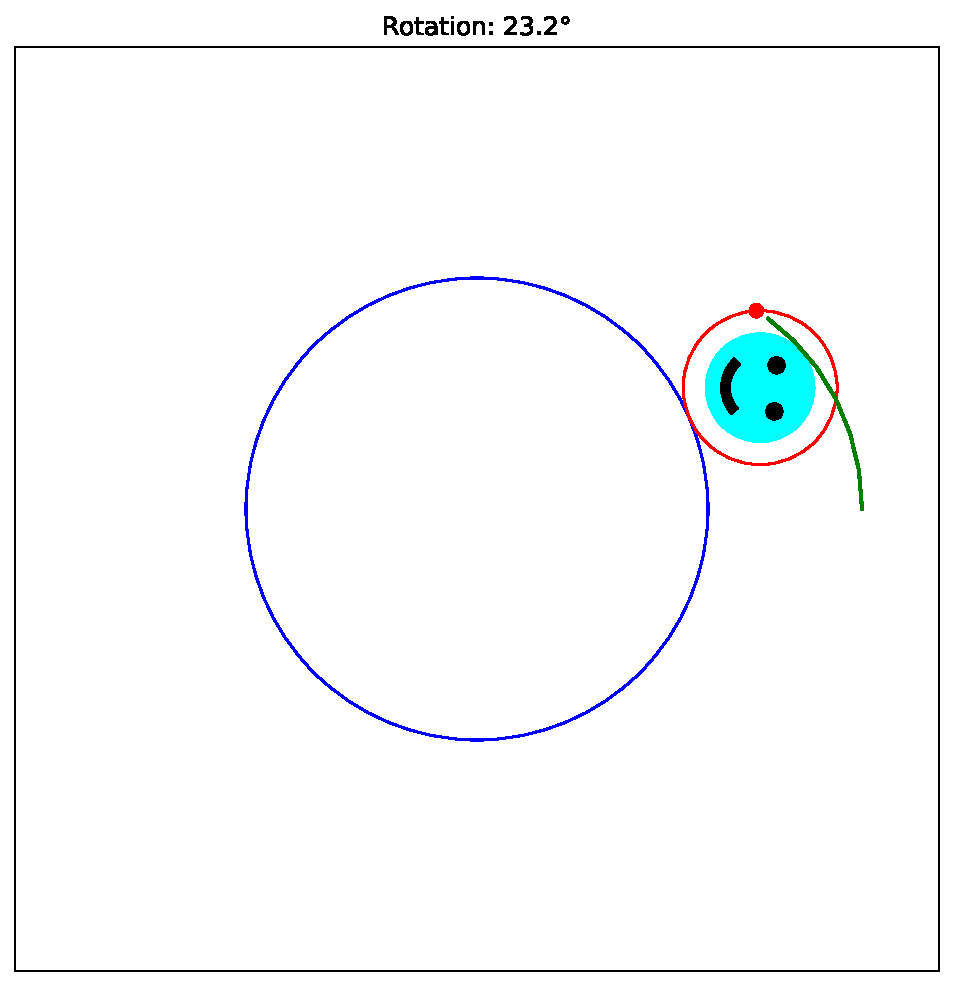
\includegraphics[width=.6\textwidth]{fig/note02/coin_rotation_33.pdf}\noindent}
\only<35>{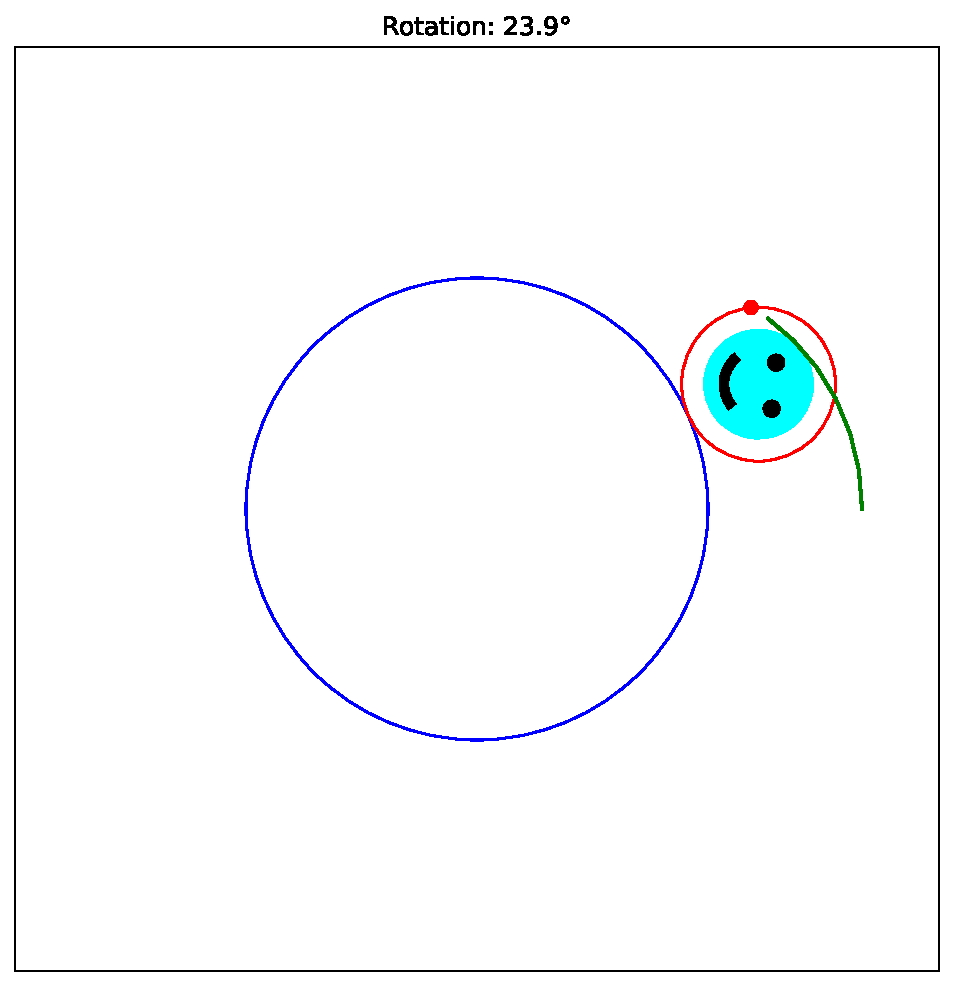
\includegraphics[width=.6\textwidth]{fig/note02/coin_rotation_34.pdf}\noindent}
\only<36>{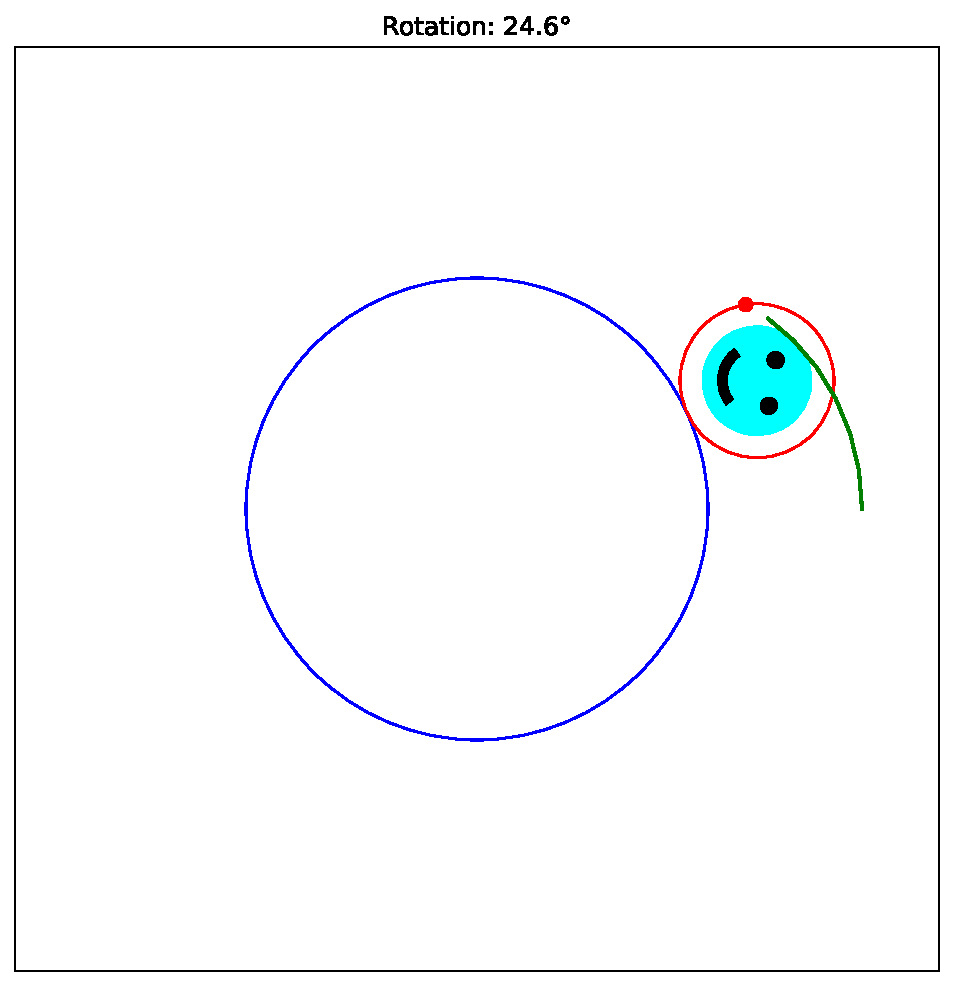
\includegraphics[width=.6\textwidth]{fig/note02/coin_rotation_35.pdf}\noindent}
\only<37>{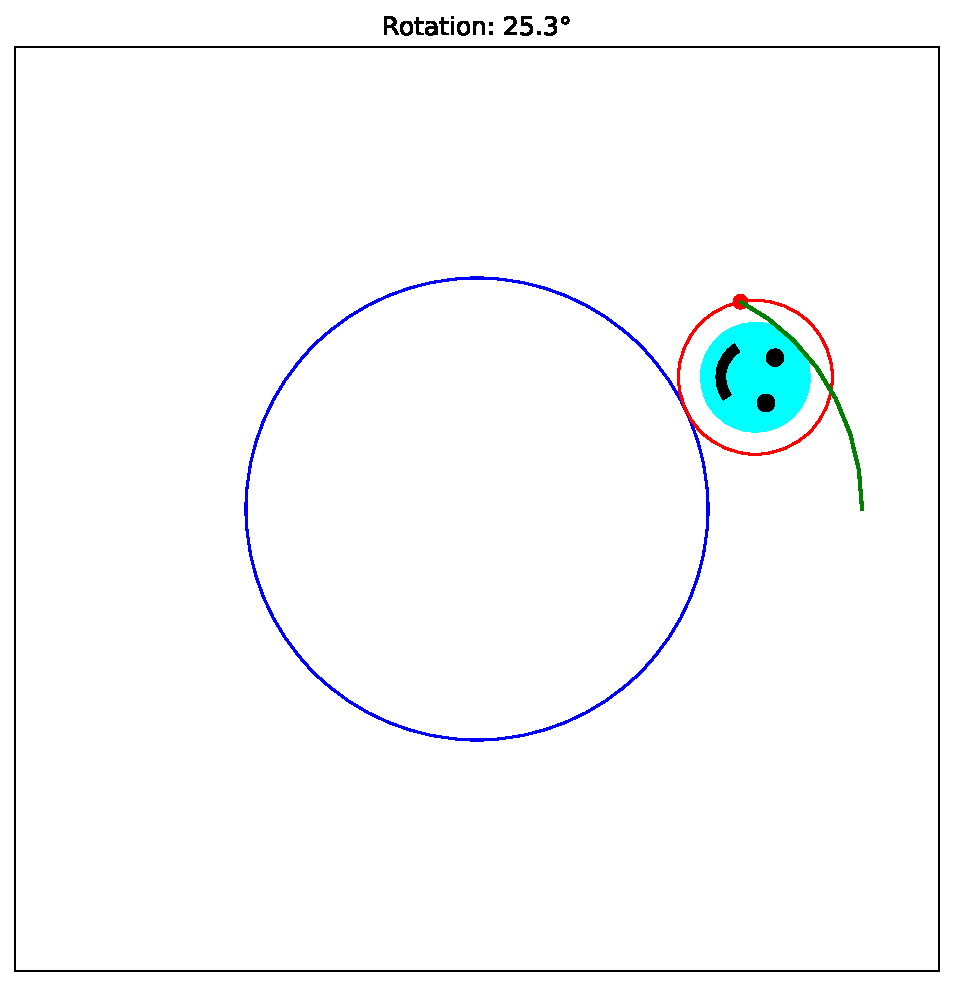
\includegraphics[width=.6\textwidth]{fig/note02/coin_rotation_36.pdf}\noindent}
\only<38>{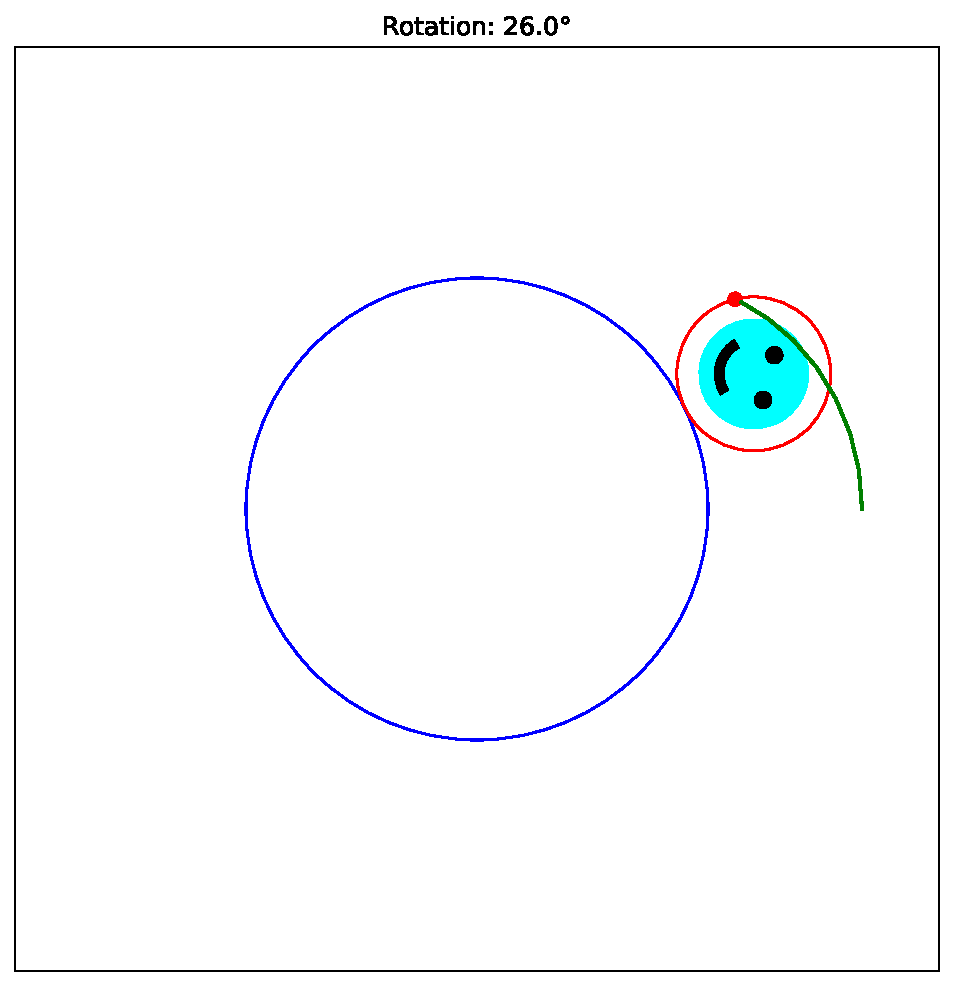
\includegraphics[width=.6\textwidth]{fig/note02/coin_rotation_37.pdf}\noindent}
\only<39>{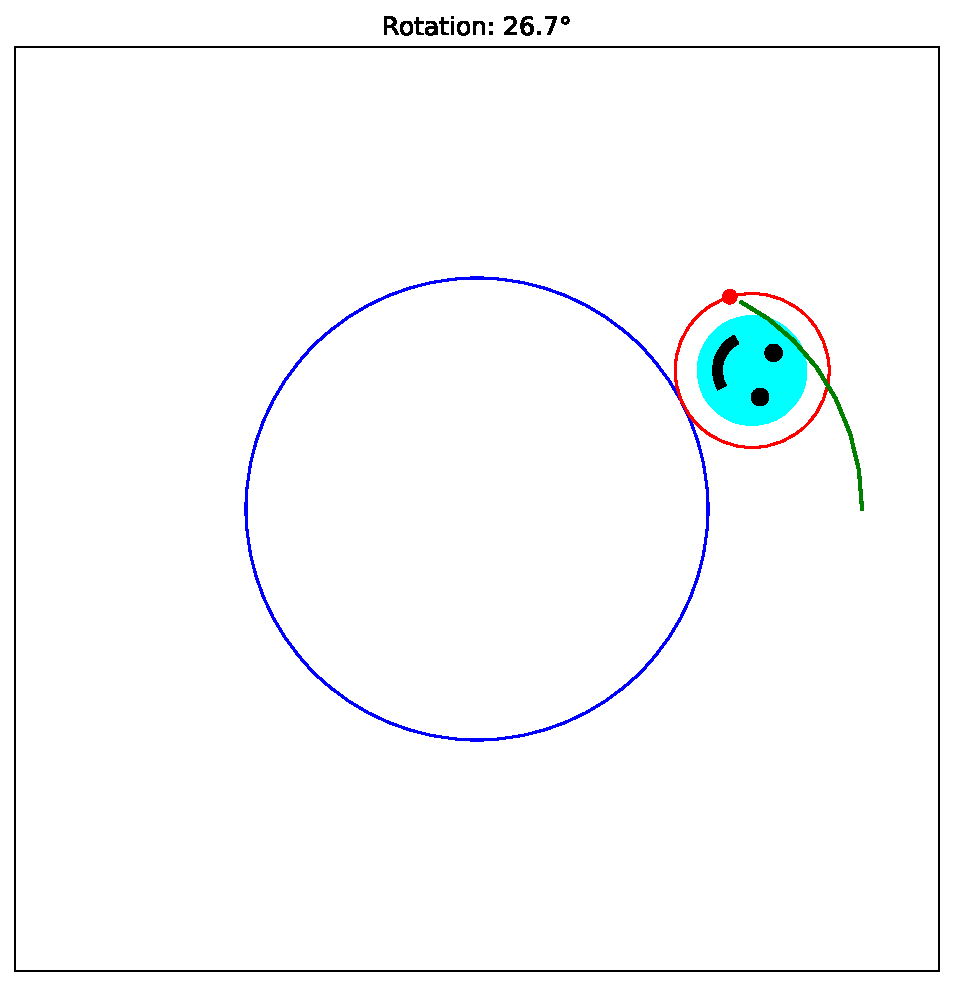
\includegraphics[width=.6\textwidth]{fig/note02/coin_rotation_38.pdf}\noindent}
\only<40>{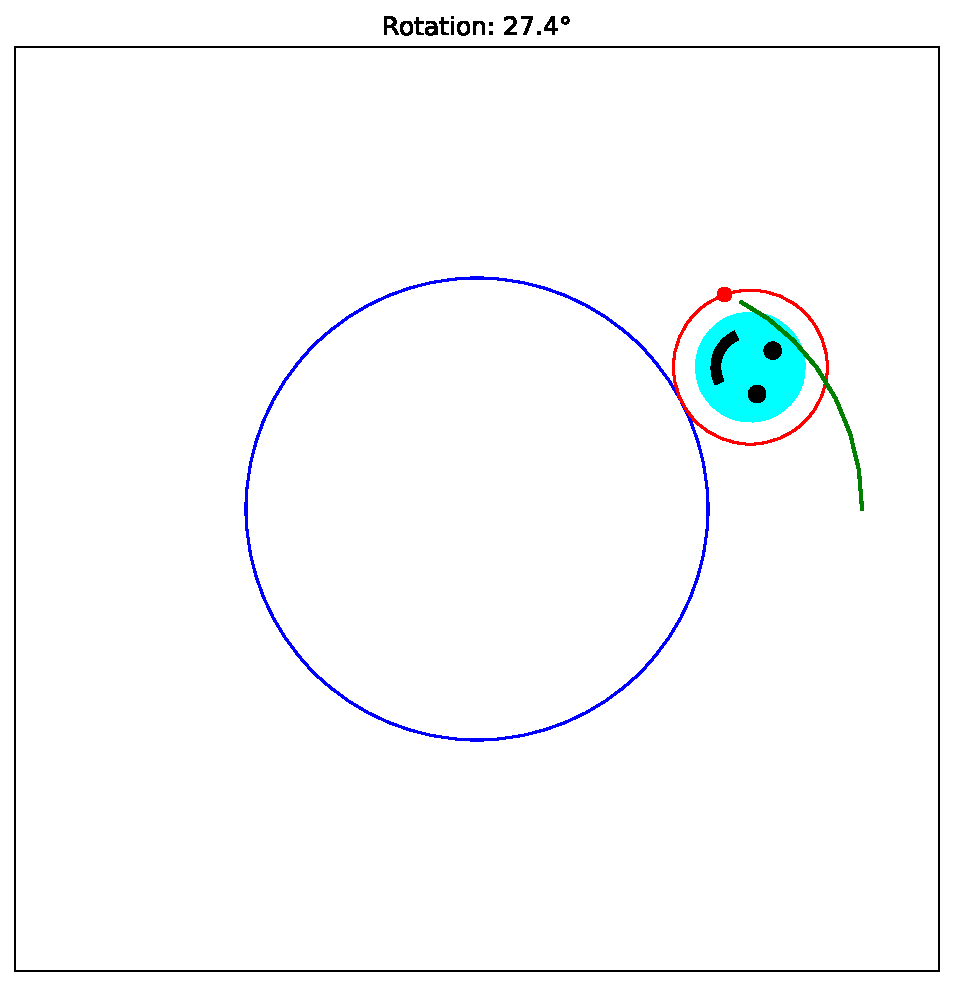
\includegraphics[width=.6\textwidth]{fig/note02/coin_rotation_39.pdf}\noindent}
\only<41>{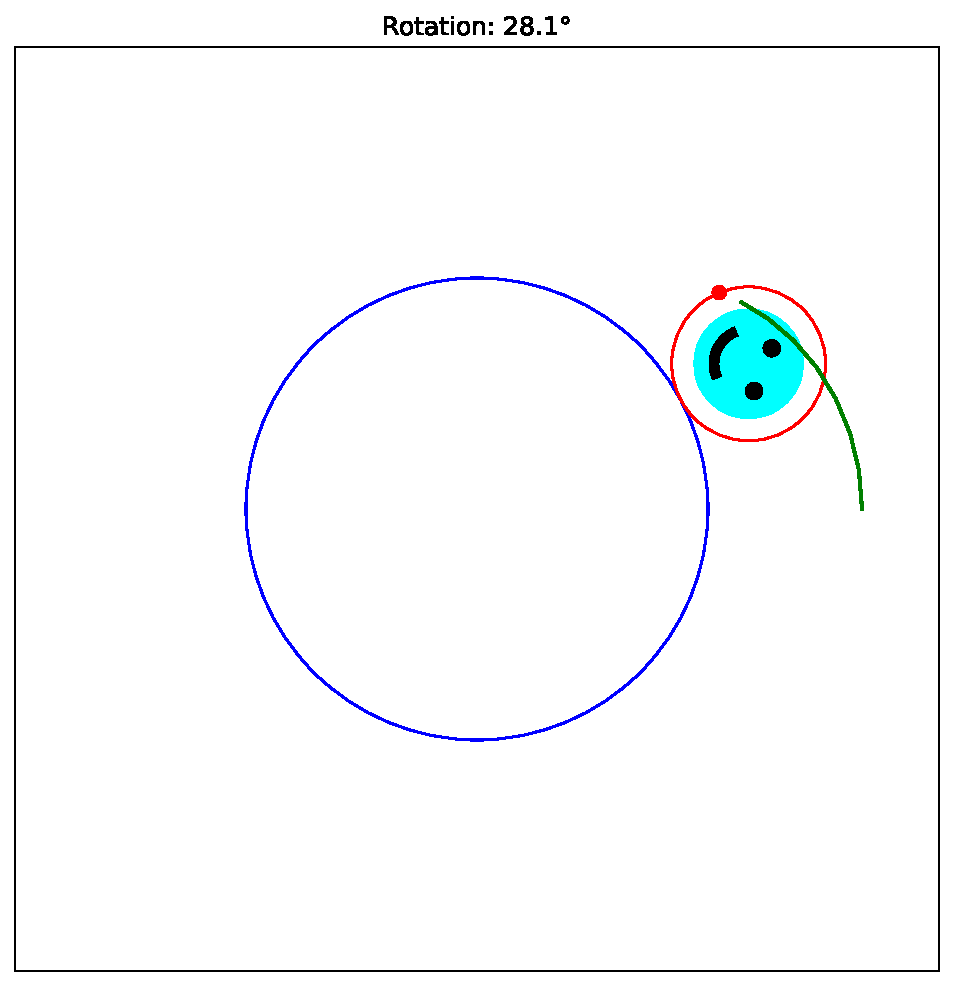
\includegraphics[width=.6\textwidth]{fig/note02/coin_rotation_40.pdf}\noindent}
\only<42>{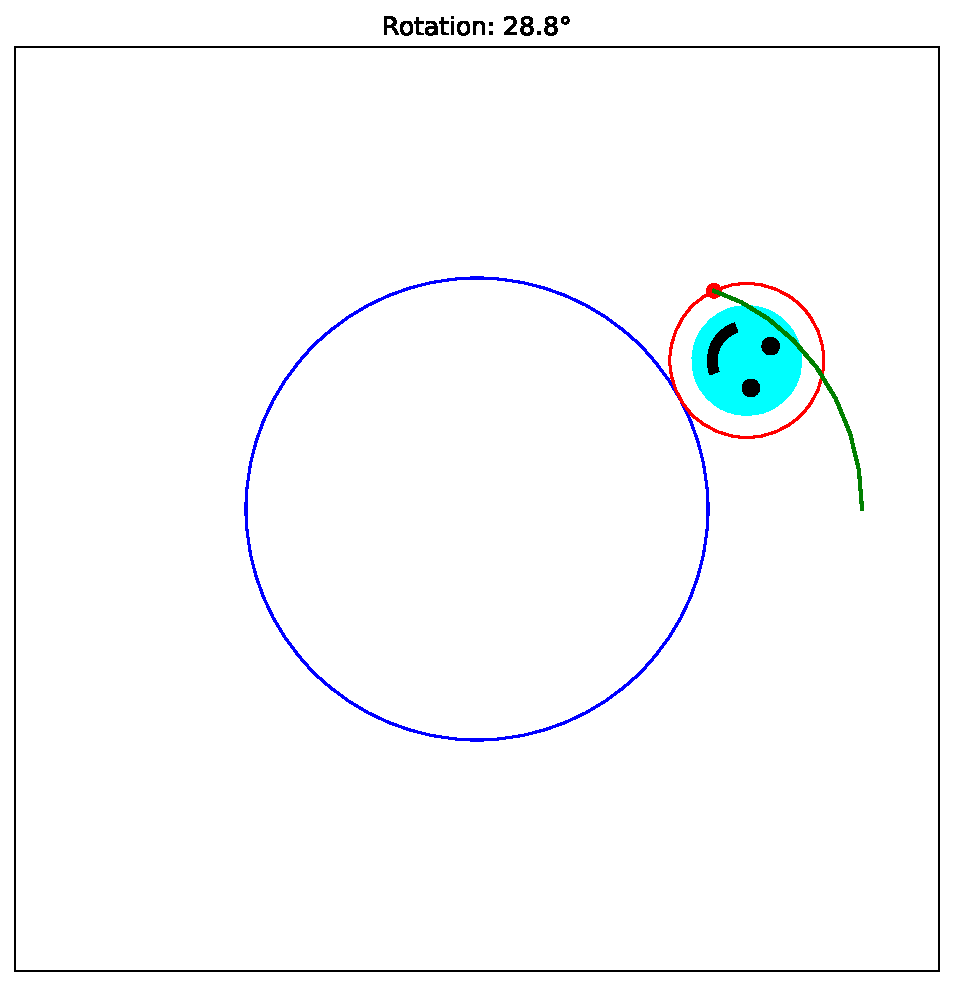
\includegraphics[width=.6\textwidth]{fig/note02/coin_rotation_41.pdf}\noindent}
\only<43>{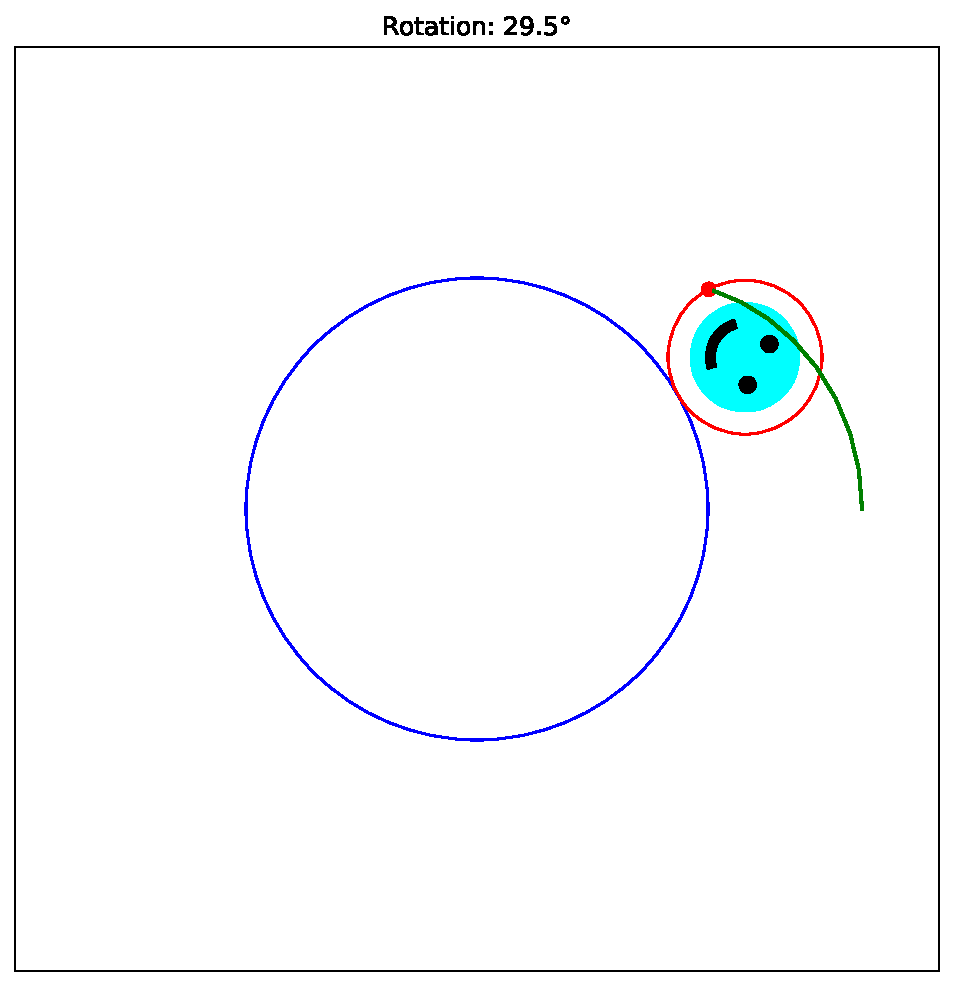
\includegraphics[width=.6\textwidth]{fig/note02/coin_rotation_42.pdf}\noindent}
\only<44>{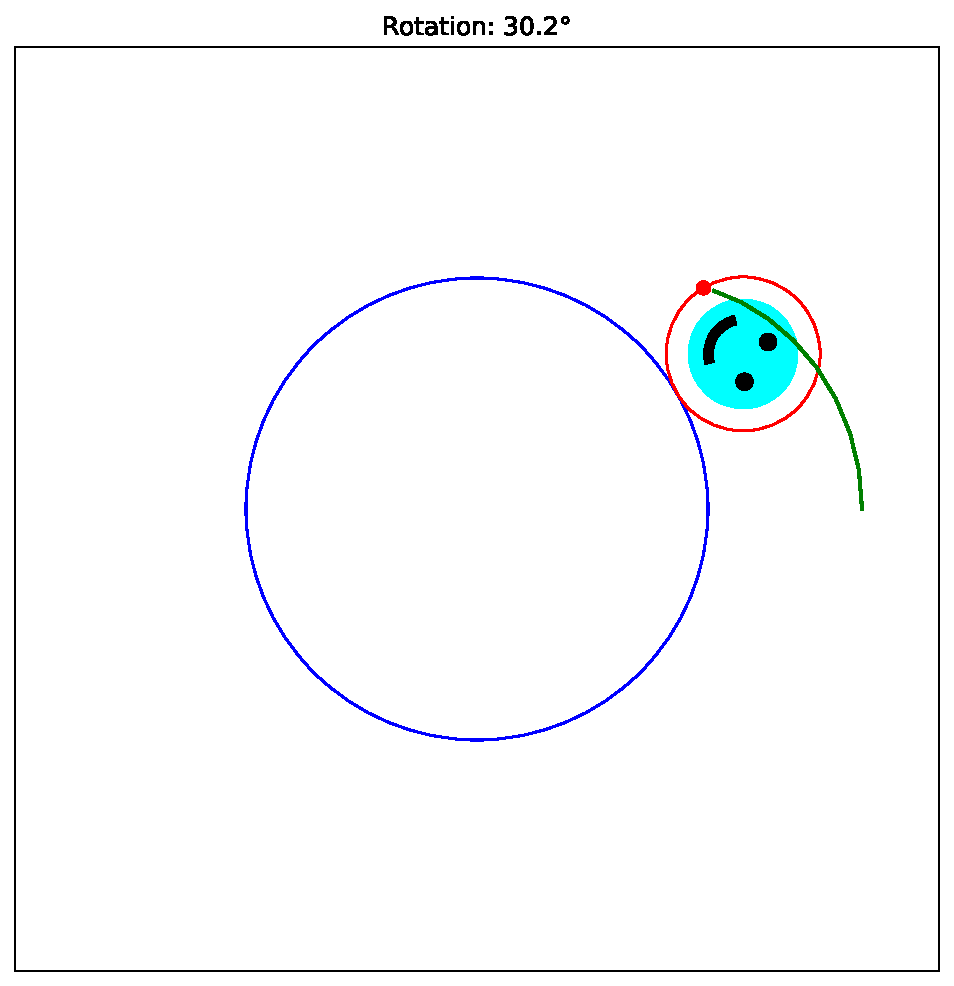
\includegraphics[width=.6\textwidth]{fig/note02/coin_rotation_43.pdf}\noindent}
\only<45>{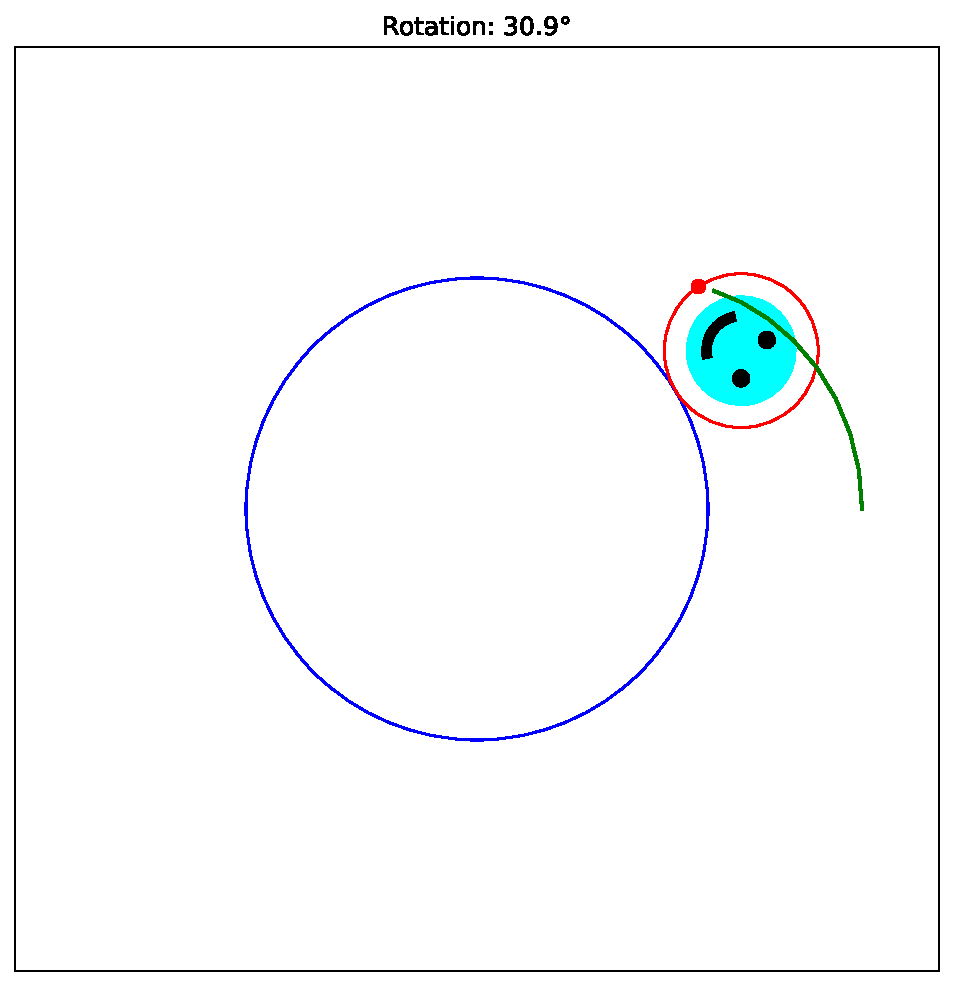
\includegraphics[width=.6\textwidth]{fig/note02/coin_rotation_44.pdf}\noindent}
\only<46>{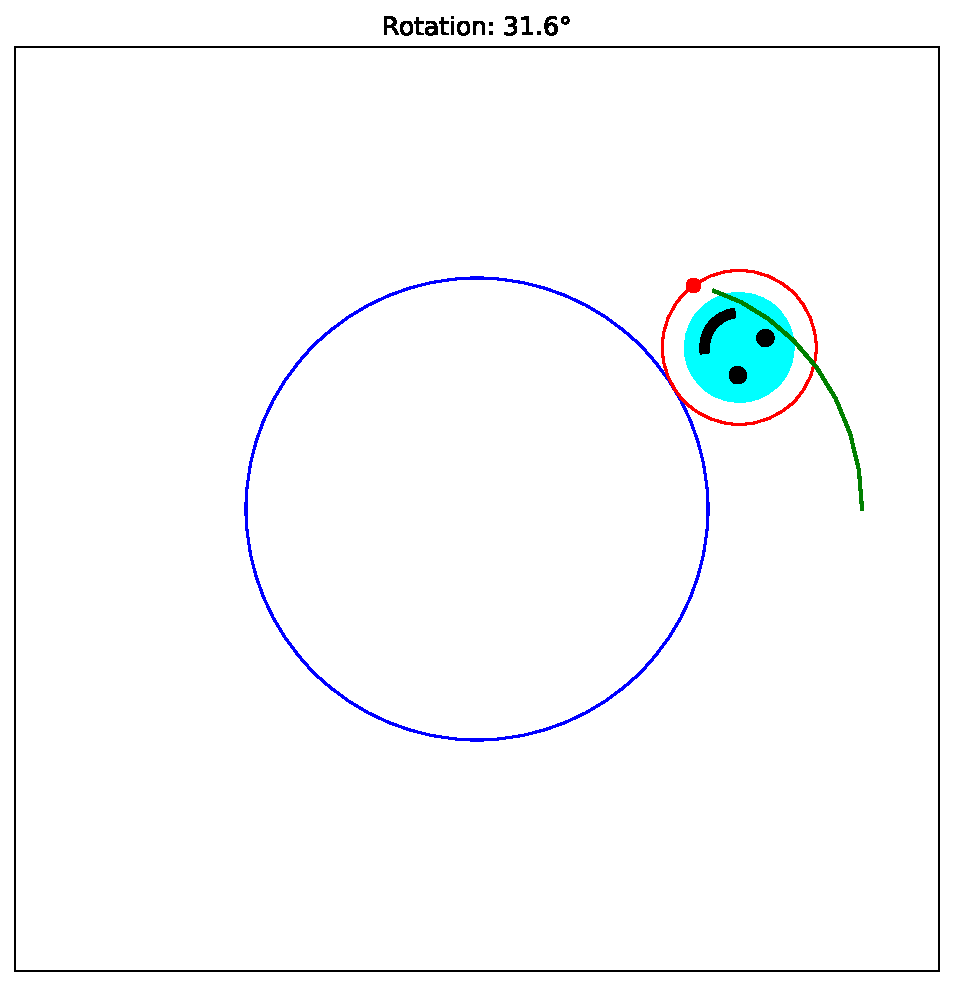
\includegraphics[width=.6\textwidth]{fig/note02/coin_rotation_45.pdf}\noindent}
\only<47>{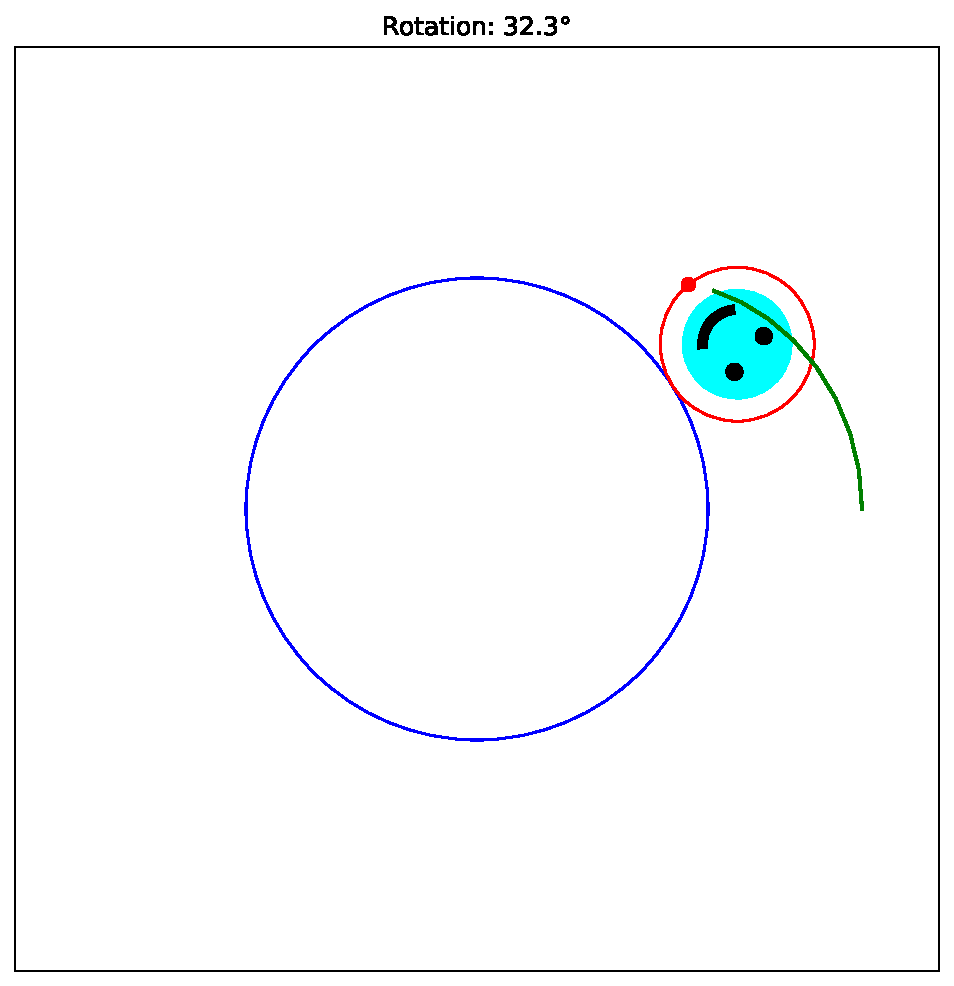
\includegraphics[width=.6\textwidth]{fig/note02/coin_rotation_46.pdf}\noindent}
\only<48>{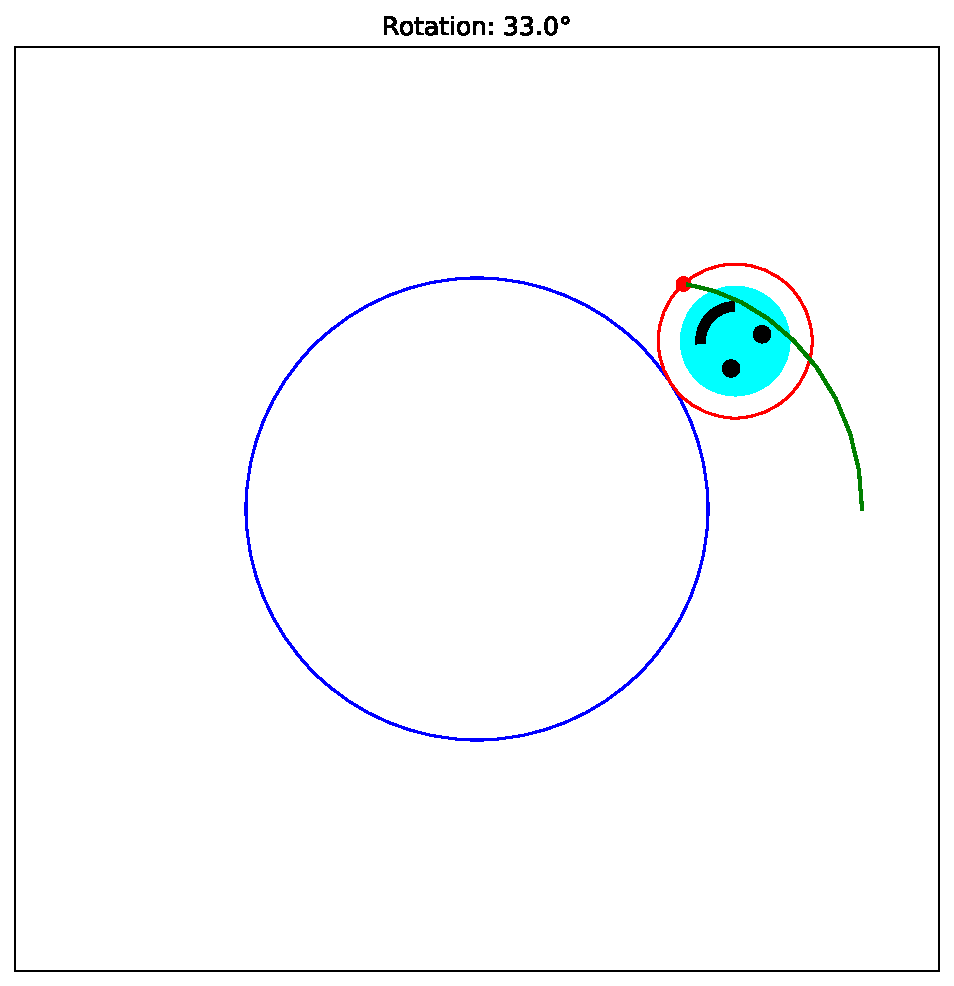
\includegraphics[width=.6\textwidth]{fig/note02/coin_rotation_47.pdf}\noindent}
\only<49>{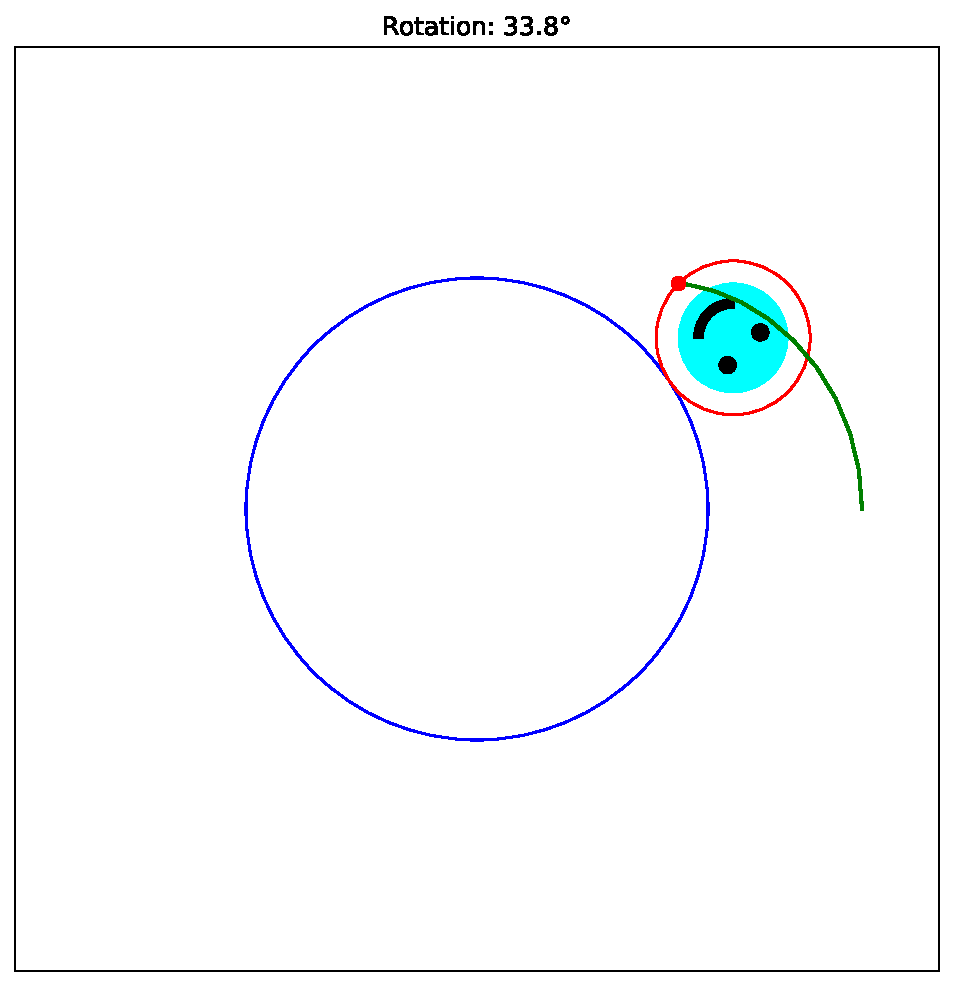
\includegraphics[width=.6\textwidth]{fig/note02/coin_rotation_48.pdf}\noindent}
\only<50>{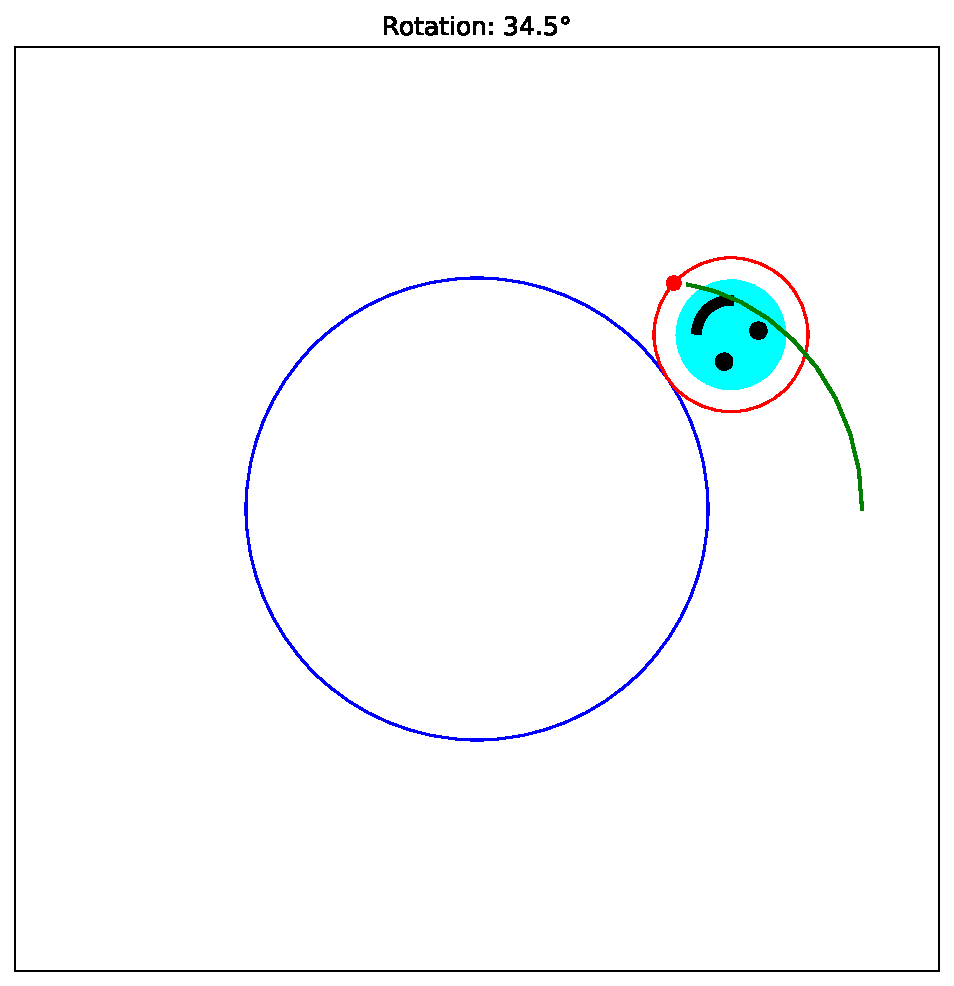
\includegraphics[width=.6\textwidth]{fig/note02/coin_rotation_49.pdf}\noindent}
\only<51>{\includegraphics[width=.6\textwidth]{fig/note02/coin_rotation_50.pdf}\noindent}
\only<52>{\includegraphics[width=.6\textwidth]{fig/note02/coin_rotation_51.pdf}\noindent}
\only<53>{\includegraphics[width=.6\textwidth]{fig/note02/coin_rotation_52.pdf}\noindent}
\only<54>{\includegraphics[width=.6\textwidth]{fig/note02/coin_rotation_53.pdf}\noindent}
\only<55>{\includegraphics[width=.6\textwidth]{fig/note02/coin_rotation_54.pdf}\noindent}
\only<56>{\includegraphics[width=.6\textwidth]{fig/note02/coin_rotation_55.pdf}\noindent}
\only<57>{\includegraphics[width=.6\textwidth]{fig/note02/coin_rotation_56.pdf}\noindent}
\only<58>{\includegraphics[width=.6\textwidth]{fig/note02/coin_rotation_57.pdf}\noindent}
\only<59>{\includegraphics[width=.6\textwidth]{fig/note02/coin_rotation_58.pdf}\noindent}
\only<60>{\includegraphics[width=.6\textwidth]{fig/note02/coin_rotation_59.pdf}\noindent}
\only<61>{\includegraphics[width=.6\textwidth]{fig/note02/coin_rotation_60.pdf}\noindent}
\only<62>{\includegraphics[width=.6\textwidth]{fig/note02/coin_rotation_61.pdf}\noindent}
\only<63>{\includegraphics[width=.6\textwidth]{fig/note02/coin_rotation_62.pdf}\noindent}
\only<64>{\includegraphics[width=.6\textwidth]{fig/note02/coin_rotation_63.pdf}\noindent}
\only<65>{\includegraphics[width=.6\textwidth]{fig/note02/coin_rotation_64.pdf}\noindent}
\only<66>{\includegraphics[width=.6\textwidth]{fig/note02/coin_rotation_65.pdf}\noindent}
\only<67>{\includegraphics[width=.6\textwidth]{fig/note02/coin_rotation_66.pdf}\noindent}
\only<68>{\includegraphics[width=.6\textwidth]{fig/note02/coin_rotation_67.pdf}\noindent}
\only<69>{\includegraphics[width=.6\textwidth]{fig/note02/coin_rotation_68.pdf}\noindent}
\only<70>{\includegraphics[width=.6\textwidth]{fig/note02/coin_rotation_69.pdf}\noindent}
\only<71>{\includegraphics[width=.6\textwidth]{fig/note02/coin_rotation_70.pdf}\noindent}
\only<72>{\includegraphics[width=.6\textwidth]{fig/note02/coin_rotation_71.pdf}\noindent}
\only<73>{\includegraphics[width=.6\textwidth]{fig/note02/coin_rotation_72.pdf}\noindent}
\only<74>{\includegraphics[width=.6\textwidth]{fig/note02/coin_rotation_73.pdf}\noindent}
\only<75>{\includegraphics[width=.6\textwidth]{fig/note02/coin_rotation_74.pdf}\noindent}
\only<76>{\includegraphics[width=.6\textwidth]{fig/note02/coin_rotation_75.pdf}\noindent}
\only<77>{\includegraphics[width=.6\textwidth]{fig/note02/coin_rotation_76.pdf}\noindent}
\only<78>{\includegraphics[width=.6\textwidth]{fig/note02/coin_rotation_77.pdf}\noindent}
\only<79>{\includegraphics[width=.6\textwidth]{fig/note02/coin_rotation_78.pdf}\noindent}
\only<80>{\includegraphics[width=.6\textwidth]{fig/note02/coin_rotation_79.pdf}\noindent}
\only<81>{\includegraphics[width=.6\textwidth]{fig/note02/coin_rotation_80.pdf}\noindent}
\only<82>{\includegraphics[width=.6\textwidth]{fig/note02/coin_rotation_81.pdf}\noindent}
\only<83>{\includegraphics[width=.6\textwidth]{fig/note02/coin_rotation_82.pdf}\noindent}
\only<84>{\includegraphics[width=.6\textwidth]{fig/note02/coin_rotation_83.pdf}\noindent}
\only<85>{\includegraphics[width=.6\textwidth]{fig/note02/coin_rotation_84.pdf}\noindent}
\only<86>{\includegraphics[width=.6\textwidth]{fig/note02/coin_rotation_85.pdf}\noindent}
\only<87>{\includegraphics[width=.6\textwidth]{fig/note02/coin_rotation_86.pdf}\noindent}
\only<88>{\includegraphics[width=.6\textwidth]{fig/note02/coin_rotation_87.pdf}\noindent}
\only<89>{\includegraphics[width=.6\textwidth]{fig/note02/coin_rotation_88.pdf}\noindent}
\only<90>{\includegraphics[width=.6\textwidth]{fig/note02/coin_rotation_89.pdf}\noindent}
\only<91>{\includegraphics[width=.6\textwidth]{fig/note02/coin_rotation_90.pdf}\noindent}
\only<92>{\includegraphics[width=.6\textwidth]{fig/note02/coin_rotation_91.pdf}\noindent}
\only<93>{\includegraphics[width=.6\textwidth]{fig/note02/coin_rotation_92.pdf}\noindent}
\only<94>{\includegraphics[width=.6\textwidth]{fig/note02/coin_rotation_93.pdf}\noindent}
\only<95>{\includegraphics[width=.6\textwidth]{fig/note02/coin_rotation_94.pdf}\noindent}
\only<96>{\includegraphics[width=.6\textwidth]{fig/note02/coin_rotation_95.pdf}\noindent}
\only<97>{\includegraphics[width=.6\textwidth]{fig/note02/coin_rotation_96.pdf}\noindent}
\only<98>{\includegraphics[width=.6\textwidth]{fig/note02/coin_rotation_97.pdf}\noindent}
\only<99>{\includegraphics[width=.6\textwidth]{fig/note02/coin_rotation_98.pdf}\noindent}
\only<100>{\includegraphics[width=.6\textwidth]{fig/note02/coin_rotation_99.pdf}\noindent}
\only<101>{\includegraphics[width=.6\textwidth]{fig/note02/coin_rotation_100.pdf}\noindent}
\only<102>{\includegraphics[width=.6\textwidth]{fig/note02/coin_rotation_101.pdf}\noindent}
\only<103>{\includegraphics[width=.6\textwidth]{fig/note02/coin_rotation_102.pdf}\noindent}
\only<104>{\includegraphics[width=.6\textwidth]{fig/note02/coin_rotation_103.pdf}\noindent}
\only<105>{\includegraphics[width=.6\textwidth]{fig/note02/coin_rotation_104.pdf}\noindent}
\only<106>{\includegraphics[width=.6\textwidth]{fig/note02/coin_rotation_105.pdf}\noindent}
\only<107>{\includegraphics[width=.6\textwidth]{fig/note02/coin_rotation_106.pdf}\noindent}
\only<108>{\includegraphics[width=.6\textwidth]{fig/note02/coin_rotation_107.pdf}\noindent}
\only<109>{\includegraphics[width=.6\textwidth]{fig/note02/coin_rotation_108.pdf}\noindent}
\only<110>{\includegraphics[width=.6\textwidth]{fig/note02/coin_rotation_109.pdf}\noindent}
\only<111>{\includegraphics[width=.6\textwidth]{fig/note02/coin_rotation_110.pdf}\noindent}
\only<112>{\includegraphics[width=.6\textwidth]{fig/note02/coin_rotation_111.pdf}\noindent}
\only<113>{\includegraphics[width=.6\textwidth]{fig/note02/coin_rotation_112.pdf}\noindent}
\only<114>{\includegraphics[width=.6\textwidth]{fig/note02/coin_rotation_113.pdf}\noindent}
\only<115>{\includegraphics[width=.6\textwidth]{fig/note02/coin_rotation_114.pdf}\noindent}
\only<116>{\includegraphics[width=.6\textwidth]{fig/note02/coin_rotation_115.pdf}\noindent}
\only<117>{\includegraphics[width=.6\textwidth]{fig/note02/coin_rotation_116.pdf}\noindent}
\only<118>{\includegraphics[width=.6\textwidth]{fig/note02/coin_rotation_117.pdf}\noindent}
\only<119>{\includegraphics[width=.6\textwidth]{fig/note02/coin_rotation_118.pdf}\noindent}
\only<120>{\includegraphics[width=.6\textwidth]{fig/note02/coin_rotation_119.pdf}\noindent}
\only<121>{\includegraphics[width=.6\textwidth]{fig/note02/coin_rotation_120.pdf}\noindent}
\only<122>{\includegraphics[width=.6\textwidth]{fig/note02/coin_rotation_121.pdf}\noindent}
\only<123>{\includegraphics[width=.6\textwidth]{fig/note02/coin_rotation_122.pdf}\noindent}
\only<124>{\includegraphics[width=.6\textwidth]{fig/note02/coin_rotation_123.pdf}\noindent}
\only<125>{\includegraphics[width=.6\textwidth]{fig/note02/coin_rotation_124.pdf}\noindent}
\only<126>{\includegraphics[width=.6\textwidth]{fig/note02/coin_rotation_125.pdf}\noindent}
\only<127>{\includegraphics[width=.6\textwidth]{fig/note02/coin_rotation_126.pdf}\noindent}
\only<128>{\includegraphics[width=.6\textwidth]{fig/note02/coin_rotation_127.pdf}\noindent}
\only<129>{\includegraphics[width=.6\textwidth]{fig/note02/coin_rotation_128.pdf}\noindent}
\only<130>{\includegraphics[width=.6\textwidth]{fig/note02/coin_rotation_129.pdf}\noindent}
\only<131>{\includegraphics[width=.6\textwidth]{fig/note02/coin_rotation_130.pdf}\noindent}
\only<132>{\includegraphics[width=.6\textwidth]{fig/note02/coin_rotation_131.pdf}\noindent}
\only<133>{\includegraphics[width=.6\textwidth]{fig/note02/coin_rotation_132.pdf}\noindent}
\only<134>{\includegraphics[width=.6\textwidth]{fig/note02/coin_rotation_133.pdf}\noindent}
\only<135>{\includegraphics[width=.6\textwidth]{fig/note02/coin_rotation_134.pdf}\noindent}
\only<136>{\includegraphics[width=.6\textwidth]{fig/note02/coin_rotation_135.pdf}\noindent}
\only<137>{\includegraphics[width=.6\textwidth]{fig/note02/coin_rotation_136.pdf}\noindent}
\only<138>{\includegraphics[width=.6\textwidth]{fig/note02/coin_rotation_137.pdf}\noindent}
\only<139>{\includegraphics[width=.6\textwidth]{fig/note02/coin_rotation_138.pdf}\noindent}
\only<140>{\includegraphics[width=.6\textwidth]{fig/note02/coin_rotation_139.pdf}\noindent}
\only<141>{\includegraphics[width=.6\textwidth]{fig/note02/coin_rotation_140.pdf}\noindent}
\only<142>{\includegraphics[width=.6\textwidth]{fig/note02/coin_rotation_141.pdf}\noindent}
\only<143>{\includegraphics[width=.6\textwidth]{fig/note02/coin_rotation_142.pdf}\noindent}
\only<144>{\includegraphics[width=.6\textwidth]{fig/note02/coin_rotation_143.pdf}\noindent}
\only<145>{\includegraphics[width=.6\textwidth]{fig/note02/coin_rotation_144.pdf}\noindent}
\only<146>{\includegraphics[width=.6\textwidth]{fig/note02/coin_rotation_145.pdf}\noindent}
\only<147>{\includegraphics[width=.6\textwidth]{fig/note02/coin_rotation_146.pdf}\noindent}
\only<148>{\includegraphics[width=.6\textwidth]{fig/note02/coin_rotation_147.pdf}\noindent}
\only<149>{\includegraphics[width=.6\textwidth]{fig/note02/coin_rotation_148.pdf}\noindent}
\only<150>{\includegraphics[width=.6\textwidth]{fig/note02/coin_rotation_149.pdf}\noindent}
\only<151>{\includegraphics[width=.6\textwidth]{fig/note02/coin_rotation_150.pdf}\noindent}
\only<152>{\includegraphics[width=.6\textwidth]{fig/note02/coin_rotation_151.pdf}\noindent}
\only<153>{\includegraphics[width=.6\textwidth]{fig/note02/coin_rotation_152.pdf}\noindent}
\only<154>{\includegraphics[width=.6\textwidth]{fig/note02/coin_rotation_153.pdf}\noindent}
\only<155>{\includegraphics[width=.6\textwidth]{fig/note02/coin_rotation_154.pdf}\noindent}
\only<156>{\includegraphics[width=.6\textwidth]{fig/note02/coin_rotation_155.pdf}\noindent}
\only<157>{\includegraphics[width=.6\textwidth]{fig/note02/coin_rotation_156.pdf}\noindent}
\only<158>{\includegraphics[width=.6\textwidth]{fig/note02/coin_rotation_157.pdf}\noindent}
\only<159>{\includegraphics[width=.6\textwidth]{fig/note02/coin_rotation_158.pdf}\noindent}
\only<160>{\includegraphics[width=.6\textwidth]{fig/note02/coin_rotation_159.pdf}\noindent}
\only<161>{\includegraphics[width=.6\textwidth]{fig/note02/coin_rotation_160.pdf}\noindent}
\only<162>{\includegraphics[width=.6\textwidth]{fig/note02/coin_rotation_161.pdf}\noindent}
\only<163>{\includegraphics[width=.6\textwidth]{fig/note02/coin_rotation_162.pdf}\noindent}
\only<164>{\includegraphics[width=.6\textwidth]{fig/note02/coin_rotation_163.pdf}\noindent}
\only<165>{\includegraphics[width=.6\textwidth]{fig/note02/coin_rotation_164.pdf}\noindent}
\only<166>{\includegraphics[width=.6\textwidth]{fig/note02/coin_rotation_165.pdf}\noindent}
\only<167>{\includegraphics[width=.6\textwidth]{fig/note02/coin_rotation_166.pdf}\noindent}
\only<168>{\includegraphics[width=.6\textwidth]{fig/note02/coin_rotation_167.pdf}\noindent}
\only<169>{\includegraphics[width=.6\textwidth]{fig/note02/coin_rotation_168.pdf}\noindent}
\only<170>{\includegraphics[width=.6\textwidth]{fig/note02/coin_rotation_169.pdf}\noindent}
\only<171>{\includegraphics[width=.6\textwidth]{fig/note02/coin_rotation_170.pdf}\noindent}
\only<172>{\includegraphics[width=.6\textwidth]{fig/note02/coin_rotation_171.pdf}\noindent}
\only<173>{\includegraphics[width=.6\textwidth]{fig/note02/coin_rotation_172.pdf}\noindent}
\only<174>{\includegraphics[width=.6\textwidth]{fig/note02/coin_rotation_173.pdf}\noindent}
\only<175>{\includegraphics[width=.6\textwidth]{fig/note02/coin_rotation_174.pdf}\noindent}
\only<176>{\includegraphics[width=.6\textwidth]{fig/note02/coin_rotation_175.pdf}\noindent}
\only<177>{\includegraphics[width=.6\textwidth]{fig/note02/coin_rotation_176.pdf}\noindent}
\only<178>{\includegraphics[width=.6\textwidth]{fig/note02/coin_rotation_177.pdf}\noindent}
\only<179>{\includegraphics[width=.6\textwidth]{fig/note02/coin_rotation_178.pdf}\noindent}
\only<180>{\includegraphics[width=.6\textwidth]{fig/note02/coin_rotation_179.pdf}\noindent}
\only<181>{\includegraphics[width=.6\textwidth]{fig/note02/coin_rotation_180.pdf}\noindent}
\only<182>{\includegraphics[width=.6\textwidth]{fig/note02/coin_rotation_181.pdf}\noindent}
\only<183>{\includegraphics[width=.6\textwidth]{fig/note02/coin_rotation_182.pdf}\noindent}
\only<184>{\includegraphics[width=.6\textwidth]{fig/note02/coin_rotation_183.pdf}\noindent}
\only<185>{\includegraphics[width=.6\textwidth]{fig/note02/coin_rotation_184.pdf}\noindent}
\only<186>{\includegraphics[width=.6\textwidth]{fig/note02/coin_rotation_185.pdf}\noindent}
\only<187>{\includegraphics[width=.6\textwidth]{fig/note02/coin_rotation_186.pdf}\noindent}
\only<188>{\includegraphics[width=.6\textwidth]{fig/note02/coin_rotation_187.pdf}\noindent}
\only<189>{\includegraphics[width=.6\textwidth]{fig/note02/coin_rotation_188.pdf}\noindent}
\only<190>{\includegraphics[width=.6\textwidth]{fig/note02/coin_rotation_189.pdf}\noindent}
\only<191>{\includegraphics[width=.6\textwidth]{fig/note02/coin_rotation_190.pdf}\noindent}
\only<192>{\includegraphics[width=.6\textwidth]{fig/note02/coin_rotation_191.pdf}\noindent}
\only<193>{\includegraphics[width=.6\textwidth]{fig/note02/coin_rotation_192.pdf}\noindent}
\only<194>{\includegraphics[width=.6\textwidth]{fig/note02/coin_rotation_193.pdf}\noindent}
\only<195>{\includegraphics[width=.6\textwidth]{fig/note02/coin_rotation_194.pdf}\noindent}
\only<196>{\includegraphics[width=.6\textwidth]{fig/note02/coin_rotation_195.pdf}\noindent}
\only<197>{\includegraphics[width=.6\textwidth]{fig/note02/coin_rotation_196.pdf}\noindent}
\only<198>{\includegraphics[width=.6\textwidth]{fig/note02/coin_rotation_197.pdf}\noindent}
\only<199>{\includegraphics[width=.6\textwidth]{fig/note02/coin_rotation_198.pdf}\noindent}
\only<200>{\includegraphics[width=.6\textwidth]{fig/note02/coin_rotation_199.pdf}\noindent}
\only<201>{\includegraphics[width=.6\textwidth]{fig/note02/coin_rotation_200.pdf}\noindent}
\only<202>{\includegraphics[width=.6\textwidth]{fig/note02/coin_rotation_201.pdf}\noindent}
\only<203>{\includegraphics[width=.6\textwidth]{fig/note02/coin_rotation_202.pdf}\noindent}
\only<204>{\includegraphics[width=.6\textwidth]{fig/note02/coin_rotation_203.pdf}\noindent}
\only<205>{\includegraphics[width=.6\textwidth]{fig/note02/coin_rotation_204.pdf}\noindent}
\only<206>{\includegraphics[width=.6\textwidth]{fig/note02/coin_rotation_205.pdf}\noindent}
\only<207>{\includegraphics[width=.6\textwidth]{fig/note02/coin_rotation_206.pdf}\noindent}
\only<208>{\includegraphics[width=.6\textwidth]{fig/note02/coin_rotation_207.pdf}\noindent}
\only<209>{\includegraphics[width=.6\textwidth]{fig/note02/coin_rotation_208.pdf}\noindent}
\only<210>{\includegraphics[width=.6\textwidth]{fig/note02/coin_rotation_209.pdf}\noindent}
\only<211>{\includegraphics[width=.6\textwidth]{fig/note02/coin_rotation_210.pdf}\noindent}
\only<212>{\includegraphics[width=.6\textwidth]{fig/note02/coin_rotation_211.pdf}\noindent}
\only<213>{\includegraphics[width=.6\textwidth]{fig/note02/coin_rotation_212.pdf}\noindent}
\only<214>{\includegraphics[width=.6\textwidth]{fig/note02/coin_rotation_213.pdf}\noindent}
\only<215>{\includegraphics[width=.6\textwidth]{fig/note02/coin_rotation_214.pdf}\noindent}
\only<216>{\includegraphics[width=.6\textwidth]{fig/note02/coin_rotation_215.pdf}\noindent}
\only<217>{\includegraphics[width=.6\textwidth]{fig/note02/coin_rotation_216.pdf}\noindent}
\only<218>{\includegraphics[width=.6\textwidth]{fig/note02/coin_rotation_217.pdf}\noindent}
\only<219>{\includegraphics[width=.6\textwidth]{fig/note02/coin_rotation_218.pdf}\noindent}
\only<220>{\includegraphics[width=.6\textwidth]{fig/note02/coin_rotation_219.pdf}\noindent}
\only<221>{\includegraphics[width=.6\textwidth]{fig/note02/coin_rotation_220.pdf}\noindent}
\only<222>{\includegraphics[width=.6\textwidth]{fig/note02/coin_rotation_221.pdf}\noindent}
\only<223>{\includegraphics[width=.6\textwidth]{fig/note02/coin_rotation_222.pdf}\noindent}
\only<224>{\includegraphics[width=.6\textwidth]{fig/note02/coin_rotation_223.pdf}\noindent}
\only<225>{\includegraphics[width=.6\textwidth]{fig/note02/coin_rotation_224.pdf}\noindent}
\only<226>{\includegraphics[width=.6\textwidth]{fig/note02/coin_rotation_225.pdf}\noindent}
\only<227>{\includegraphics[width=.6\textwidth]{fig/note02/coin_rotation_226.pdf}\noindent}
\only<228>{\includegraphics[width=.6\textwidth]{fig/note02/coin_rotation_227.pdf}\noindent}
\only<229>{\includegraphics[width=.6\textwidth]{fig/note02/coin_rotation_228.pdf}\noindent}
\only<230>{\includegraphics[width=.6\textwidth]{fig/note02/coin_rotation_229.pdf}\noindent}
\only<231>{\includegraphics[width=.6\textwidth]{fig/note02/coin_rotation_230.pdf}\noindent}
\only<232>{\includegraphics[width=.6\textwidth]{fig/note02/coin_rotation_231.pdf}\noindent}
\only<233>{\includegraphics[width=.6\textwidth]{fig/note02/coin_rotation_232.pdf}\noindent}
\only<234>{\includegraphics[width=.6\textwidth]{fig/note02/coin_rotation_233.pdf}\noindent}
\only<235>{\includegraphics[width=.6\textwidth]{fig/note02/coin_rotation_234.pdf}\noindent}
\only<236>{\includegraphics[width=.6\textwidth]{fig/note02/coin_rotation_235.pdf}\noindent}
\only<237>{\includegraphics[width=.6\textwidth]{fig/note02/coin_rotation_236.pdf}\noindent}
\only<238>{\includegraphics[width=.6\textwidth]{fig/note02/coin_rotation_237.pdf}\noindent}
\only<239>{\includegraphics[width=.6\textwidth]{fig/note02/coin_rotation_238.pdf}\noindent}
\only<240>{\includegraphics[width=.6\textwidth]{fig/note02/coin_rotation_239.pdf}\noindent}
\only<241>{\includegraphics[width=.6\textwidth]{fig/note02/coin_rotation_240.pdf}\noindent}
\only<242>{\includegraphics[width=.6\textwidth]{fig/note02/coin_rotation_241.pdf}\noindent}
\only<243>{\includegraphics[width=.6\textwidth]{fig/note02/coin_rotation_242.pdf}\noindent}
\only<244>{\includegraphics[width=.6\textwidth]{fig/note02/coin_rotation_243.pdf}\noindent}
\only<245>{\includegraphics[width=.6\textwidth]{fig/note02/coin_rotation_244.pdf}\noindent}
\only<246>{\includegraphics[width=.6\textwidth]{fig/note02/coin_rotation_245.pdf}\noindent}
\only<247>{\includegraphics[width=.6\textwidth]{fig/note02/coin_rotation_246.pdf}\noindent}
\only<248>{\includegraphics[width=.6\textwidth]{fig/note02/coin_rotation_247.pdf}\noindent}
\only<249>{\includegraphics[width=.6\textwidth]{fig/note02/coin_rotation_248.pdf}\noindent}
\only<250>{\includegraphics[width=.6\textwidth]{fig/note02/coin_rotation_249.pdf}\noindent}
\only<251>{\includegraphics[width=.6\textwidth]{fig/note02/coin_rotation_250.pdf}\noindent}
\only<252>{\includegraphics[width=.6\textwidth]{fig/note02/coin_rotation_251.pdf}\noindent}
\only<253>{\includegraphics[width=.6\textwidth]{fig/note02/coin_rotation_252.pdf}\noindent}
\only<254>{\includegraphics[width=.6\textwidth]{fig/note02/coin_rotation_253.pdf}\noindent}
\only<255>{\includegraphics[width=.6\textwidth]{fig/note02/coin_rotation_254.pdf}\noindent}
\only<256>{\includegraphics[width=.6\textwidth]{fig/note02/coin_rotation_255.pdf}\noindent}
\only<257>{\includegraphics[width=.6\textwidth]{fig/note02/coin_rotation_256.pdf}\noindent}
\only<258>{\includegraphics[width=.6\textwidth]{fig/note02/coin_rotation_257.pdf}\noindent}
\only<259>{\includegraphics[width=.6\textwidth]{fig/note02/coin_rotation_258.pdf}\noindent}
\only<260>{\includegraphics[width=.6\textwidth]{fig/note02/coin_rotation_259.pdf}\noindent}
\only<261>{\includegraphics[width=.6\textwidth]{fig/note02/coin_rotation_260.pdf}\noindent}
\only<262>{\includegraphics[width=.6\textwidth]{fig/note02/coin_rotation_261.pdf}\noindent}
\only<263>{\includegraphics[width=.6\textwidth]{fig/note02/coin_rotation_262.pdf}\noindent}
\only<264>{\includegraphics[width=.6\textwidth]{fig/note02/coin_rotation_263.pdf}\noindent}
\only<265>{\includegraphics[width=.6\textwidth]{fig/note02/coin_rotation_264.pdf}\noindent}
\only<266>{\includegraphics[width=.6\textwidth]{fig/note02/coin_rotation_265.pdf}\noindent}
\only<267>{\includegraphics[width=.6\textwidth]{fig/note02/coin_rotation_266.pdf}\noindent}
\only<268>{\includegraphics[width=.6\textwidth]{fig/note02/coin_rotation_267.pdf}\noindent}
\only<269>{\includegraphics[width=.6\textwidth]{fig/note02/coin_rotation_268.pdf}\noindent}
\only<270>{\includegraphics[width=.6\textwidth]{fig/note02/coin_rotation_269.pdf}\noindent}
\only<271>{\includegraphics[width=.6\textwidth]{fig/note02/coin_rotation_270.pdf}\noindent}
\only<272>{\includegraphics[width=.6\textwidth]{fig/note02/coin_rotation_271.pdf}\noindent}
\only<273>{\includegraphics[width=.6\textwidth]{fig/note02/coin_rotation_272.pdf}\noindent}
\only<274>{\includegraphics[width=.6\textwidth]{fig/note02/coin_rotation_273.pdf}\noindent}
\only<275>{\includegraphics[width=.6\textwidth]{fig/note02/coin_rotation_274.pdf}\noindent}
\only<276>{\includegraphics[width=.6\textwidth]{fig/note02/coin_rotation_275.pdf}\noindent}
\only<277>{\includegraphics[width=.6\textwidth]{fig/note02/coin_rotation_276.pdf}\noindent}
\only<278>{\includegraphics[width=.6\textwidth]{fig/note02/coin_rotation_277.pdf}\noindent}
\only<279>{\includegraphics[width=.6\textwidth]{fig/note02/coin_rotation_278.pdf}\noindent}
\only<280>{\includegraphics[width=.6\textwidth]{fig/note02/coin_rotation_279.pdf}\noindent}
\only<281>{\includegraphics[width=.6\textwidth]{fig/note02/coin_rotation_280.pdf}\noindent}
\only<282>{\includegraphics[width=.6\textwidth]{fig/note02/coin_rotation_281.pdf}\noindent}
\only<283>{\includegraphics[width=.6\textwidth]{fig/note02/coin_rotation_282.pdf}\noindent}
\only<284>{\includegraphics[width=.6\textwidth]{fig/note02/coin_rotation_283.pdf}\noindent}
\only<285>{\includegraphics[width=.6\textwidth]{fig/note02/coin_rotation_284.pdf}\noindent}
\only<286>{\includegraphics[width=.6\textwidth]{fig/note02/coin_rotation_285.pdf}\noindent}
\only<287>{\includegraphics[width=.6\textwidth]{fig/note02/coin_rotation_286.pdf}\noindent}
\only<288>{\includegraphics[width=.6\textwidth]{fig/note02/coin_rotation_287.pdf}\noindent}
\only<289>{\includegraphics[width=.6\textwidth]{fig/note02/coin_rotation_288.pdf}\noindent}
\only<290>{\includegraphics[width=.6\textwidth]{fig/note02/coin_rotation_289.pdf}\noindent}
\only<291>{\includegraphics[width=.6\textwidth]{fig/note02/coin_rotation_290.pdf}\noindent}
\only<292>{\includegraphics[width=.6\textwidth]{fig/note02/coin_rotation_291.pdf}\noindent}
\only<293>{\includegraphics[width=.6\textwidth]{fig/note02/coin_rotation_292.pdf}\noindent}
\only<294>{\includegraphics[width=.6\textwidth]{fig/note02/coin_rotation_293.pdf}\noindent}
\only<295>{\includegraphics[width=.6\textwidth]{fig/note02/coin_rotation_294.pdf}\noindent}
\only<296>{\includegraphics[width=.6\textwidth]{fig/note02/coin_rotation_295.pdf}\noindent}
\only<297>{\includegraphics[width=.6\textwidth]{fig/note02/coin_rotation_296.pdf}\noindent}
\only<298>{\includegraphics[width=.6\textwidth]{fig/note02/coin_rotation_297.pdf}\noindent}
\only<299>{\includegraphics[width=.6\textwidth]{fig/note02/coin_rotation_298.pdf}\noindent}
\only<300>{\includegraphics[width=.6\textwidth]{fig/note02/coin_rotation_299.pdf}\noindent}
\only<301>{\includegraphics[width=.6\textwidth]{fig/note02/coin_rotation_300.pdf}\noindent}
\only<302>{\includegraphics[width=.6\textwidth]{fig/note02/coin_rotation_301.pdf}\noindent}
\only<303>{\includegraphics[width=.6\textwidth]{fig/note02/coin_rotation_302.pdf}\noindent}
\only<304>{\includegraphics[width=.6\textwidth]{fig/note02/coin_rotation_303.pdf}\noindent}
\only<305>{\includegraphics[width=.6\textwidth]{fig/note02/coin_rotation_304.pdf}\noindent}
\only<306>{\includegraphics[width=.6\textwidth]{fig/note02/coin_rotation_305.pdf}\noindent}
\only<307>{\includegraphics[width=.6\textwidth]{fig/note02/coin_rotation_306.pdf}\noindent}
\only<308>{\includegraphics[width=.6\textwidth]{fig/note02/coin_rotation_307.pdf}\noindent}
\only<309>{\includegraphics[width=.6\textwidth]{fig/note02/coin_rotation_308.pdf}\noindent}
\only<310>{\includegraphics[width=.6\textwidth]{fig/note02/coin_rotation_309.pdf}\noindent}
\only<311>{\includegraphics[width=.6\textwidth]{fig/note02/coin_rotation_310.pdf}\noindent}
\only<312>{\includegraphics[width=.6\textwidth]{fig/note02/coin_rotation_311.pdf}\noindent}
\only<313>{\includegraphics[width=.6\textwidth]{fig/note02/coin_rotation_312.pdf}\noindent}
\only<314>{\includegraphics[width=.6\textwidth]{fig/note02/coin_rotation_313.pdf}\noindent}
\only<315>{\includegraphics[width=.6\textwidth]{fig/note02/coin_rotation_314.pdf}\noindent}
\only<316>{\includegraphics[width=.6\textwidth]{fig/note02/coin_rotation_315.pdf}\noindent}
\only<317>{\includegraphics[width=.6\textwidth]{fig/note02/coin_rotation_316.pdf}\noindent}
\only<318>{\includegraphics[width=.6\textwidth]{fig/note02/coin_rotation_317.pdf}\noindent}
\only<319>{\includegraphics[width=.6\textwidth]{fig/note02/coin_rotation_318.pdf}\noindent}
\only<320>{\includegraphics[width=.6\textwidth]{fig/note02/coin_rotation_319.pdf}\noindent}
\only<321>{\includegraphics[width=.6\textwidth]{fig/note02/coin_rotation_320.pdf}\noindent}
\only<322>{\includegraphics[width=.6\textwidth]{fig/note02/coin_rotation_321.pdf}\noindent}
\only<323>{\includegraphics[width=.6\textwidth]{fig/note02/coin_rotation_322.pdf}\noindent}
\only<324>{\includegraphics[width=.6\textwidth]{fig/note02/coin_rotation_323.pdf}\noindent}
\only<325>{\includegraphics[width=.6\textwidth]{fig/note02/coin_rotation_324.pdf}\noindent}
\only<326>{\includegraphics[width=.6\textwidth]{fig/note02/coin_rotation_325.pdf}\noindent}
\only<327>{\includegraphics[width=.6\textwidth]{fig/note02/coin_rotation_326.pdf}\noindent}
\only<328>{\includegraphics[width=.6\textwidth]{fig/note02/coin_rotation_327.pdf}\noindent}
\only<329>{\includegraphics[width=.6\textwidth]{fig/note02/coin_rotation_328.pdf}\noindent}
\only<330>{\includegraphics[width=.6\textwidth]{fig/note02/coin_rotation_329.pdf}\noindent}
\only<331>{\includegraphics[width=.6\textwidth]{fig/note02/coin_rotation_330.pdf}\noindent}
\only<332>{\includegraphics[width=.6\textwidth]{fig/note02/coin_rotation_331.pdf}\noindent}
\only<333>{\includegraphics[width=.6\textwidth]{fig/note02/coin_rotation_332.pdf}\noindent}
\only<334>{\includegraphics[width=.6\textwidth]{fig/note02/coin_rotation_333.pdf}\noindent}
\only<335>{\includegraphics[width=.6\textwidth]{fig/note02/coin_rotation_334.pdf}\noindent}
\only<336>{\includegraphics[width=.6\textwidth]{fig/note02/coin_rotation_335.pdf}\noindent}
\only<337>{\includegraphics[width=.6\textwidth]{fig/note02/coin_rotation_336.pdf}\noindent}
\only<338>{\includegraphics[width=.6\textwidth]{fig/note02/coin_rotation_337.pdf}\noindent}
\only<339>{\includegraphics[width=.6\textwidth]{fig/note02/coin_rotation_338.pdf}\noindent}
\only<340>{\includegraphics[width=.6\textwidth]{fig/note02/coin_rotation_339.pdf}\noindent}
\only<341>{\includegraphics[width=.6\textwidth]{fig/note02/coin_rotation_340.pdf}\noindent}
\only<342>{\includegraphics[width=.6\textwidth]{fig/note02/coin_rotation_341.pdf}\noindent}
\only<343>{\includegraphics[width=.6\textwidth]{fig/note02/coin_rotation_342.pdf}\noindent}
\only<344>{\includegraphics[width=.6\textwidth]{fig/note02/coin_rotation_343.pdf}\noindent}
\only<345>{\includegraphics[width=.6\textwidth]{fig/note02/coin_rotation_344.pdf}\noindent}
\only<346>{\includegraphics[width=.6\textwidth]{fig/note02/coin_rotation_345.pdf}\noindent}
\only<347>{\includegraphics[width=.6\textwidth]{fig/note02/coin_rotation_346.pdf}\noindent}
\only<348>{\includegraphics[width=.6\textwidth]{fig/note02/coin_rotation_347.pdf}\noindent}
\only<349>{\includegraphics[width=.6\textwidth]{fig/note02/coin_rotation_348.pdf}\noindent}
\only<350>{\includegraphics[width=.6\textwidth]{fig/note02/coin_rotation_349.pdf}\noindent}
\only<351>{\includegraphics[width=.6\textwidth]{fig/note02/coin_rotation_350.pdf}\noindent}
\only<352>{\includegraphics[width=.6\textwidth]{fig/note02/coin_rotation_351.pdf}\noindent}
\only<353>{\includegraphics[width=.6\textwidth]{fig/note02/coin_rotation_352.pdf}\noindent}
\only<354>{\includegraphics[width=.6\textwidth]{fig/note02/coin_rotation_353.pdf}\noindent}
\only<355>{\includegraphics[width=.6\textwidth]{fig/note02/coin_rotation_354.pdf}\noindent}
\only<356>{\includegraphics[width=.6\textwidth]{fig/note02/coin_rotation_355.pdf}\noindent}
\only<357>{\includegraphics[width=.6\textwidth]{fig/note02/coin_rotation_356.pdf}\noindent}
\only<358>{\includegraphics[width=.6\textwidth]{fig/note02/coin_rotation_357.pdf}\noindent}
\only<359>{\includegraphics[width=.6\textwidth]{fig/note02/coin_rotation_358.pdf}\noindent}
\only<360>{\includegraphics[width=.6\textwidth]{fig/note02/coin_rotation_359.pdf}\noindent}
\only<361>{\includegraphics[width=.6\textwidth]{fig/note02/coin_rotation_360.pdf}\noindent}
\only<362>{\includegraphics[width=.6\textwidth]{fig/note02/coin_rotation_361.pdf}\noindent}
\only<363>{\includegraphics[width=.6\textwidth]{fig/note02/coin_rotation_362.pdf}\noindent}
\only<364>{\includegraphics[width=.6\textwidth]{fig/note02/coin_rotation_363.pdf}\noindent}
\only<365>{\includegraphics[width=.6\textwidth]{fig/note02/coin_rotation_364.pdf}\noindent}
\only<366>{\includegraphics[width=.6\textwidth]{fig/note02/coin_rotation_365.pdf}\noindent}
\only<367>{\includegraphics[width=.6\textwidth]{fig/note02/coin_rotation_366.pdf}\noindent}
\only<368>{\includegraphics[width=.6\textwidth]{fig/note02/coin_rotation_367.pdf}\noindent}
\only<369>{\includegraphics[width=.6\textwidth]{fig/note02/coin_rotation_368.pdf}\noindent}
\only<370>{\includegraphics[width=.6\textwidth]{fig/note02/coin_rotation_369.pdf}\noindent}
\only<371>{\includegraphics[width=.6\textwidth]{fig/note02/coin_rotation_370.pdf}\noindent}
\only<372>{\includegraphics[width=.6\textwidth]{fig/note02/coin_rotation_371.pdf}\noindent}
\only<373>{\includegraphics[width=.6\textwidth]{fig/note02/coin_rotation_372.pdf}\noindent}
\only<374>{\includegraphics[width=.6\textwidth]{fig/note02/coin_rotation_373.pdf}\noindent}
\only<375>{\includegraphics[width=.6\textwidth]{fig/note02/coin_rotation_374.pdf}\noindent}
\only<376>{\includegraphics[width=.6\textwidth]{fig/note02/coin_rotation_375.pdf}\noindent}
\only<377>{\includegraphics[width=.6\textwidth]{fig/note02/coin_rotation_376.pdf}\noindent}
\only<378>{\includegraphics[width=.6\textwidth]{fig/note02/coin_rotation_377.pdf}\noindent}
\only<379>{\includegraphics[width=.6\textwidth]{fig/note02/coin_rotation_378.pdf}\noindent}
\only<380>{\includegraphics[width=.6\textwidth]{fig/note02/coin_rotation_379.pdf}\noindent}
\only<381>{\includegraphics[width=.6\textwidth]{fig/note02/coin_rotation_380.pdf}\noindent}
\only<382>{\includegraphics[width=.6\textwidth]{fig/note02/coin_rotation_381.pdf}\noindent}
\only<383>{\includegraphics[width=.6\textwidth]{fig/note02/coin_rotation_382.pdf}\noindent}
\only<384>{\includegraphics[width=.6\textwidth]{fig/note02/coin_rotation_383.pdf}\noindent}
\only<385>{\includegraphics[width=.6\textwidth]{fig/note02/coin_rotation_384.pdf}\noindent}
\only<386>{\includegraphics[width=.6\textwidth]{fig/note02/coin_rotation_385.pdf}\noindent}
\only<387>{\includegraphics[width=.6\textwidth]{fig/note02/coin_rotation_386.pdf}\noindent}
\only<388>{\includegraphics[width=.6\textwidth]{fig/note02/coin_rotation_387.pdf}\noindent}
\only<389>{\includegraphics[width=.6\textwidth]{fig/note02/coin_rotation_388.pdf}\noindent}
\only<390>{\includegraphics[width=.6\textwidth]{fig/note02/coin_rotation_389.pdf}\noindent}
\only<391>{\includegraphics[width=.6\textwidth]{fig/note02/coin_rotation_390.pdf}\noindent}
\only<392>{\includegraphics[width=.6\textwidth]{fig/note02/coin_rotation_391.pdf}\noindent}
\only<393>{\includegraphics[width=.6\textwidth]{fig/note02/coin_rotation_392.pdf}\noindent}
\only<394>{\includegraphics[width=.6\textwidth]{fig/note02/coin_rotation_393.pdf}\noindent}
\only<395>{\includegraphics[width=.6\textwidth]{fig/note02/coin_rotation_394.pdf}\noindent}
\only<396>{\includegraphics[width=.6\textwidth]{fig/note02/coin_rotation_395.pdf}\noindent}
\only<397>{\includegraphics[width=.6\textwidth]{fig/note02/coin_rotation_396.pdf}\noindent}
\only<398>{\includegraphics[width=.6\textwidth]{fig/note02/coin_rotation_397.pdf}\noindent}
\only<399>{\includegraphics[width=.6\textwidth]{fig/note02/coin_rotation_398.pdf}\noindent}
\only<400>{\includegraphics[width=.6\textwidth]{fig/note02/coin_rotation_399.pdf}\noindent}
\only<401>{\includegraphics[width=.6\textwidth]{fig/note02/coin_rotation_400.pdf}\noindent}
\only<402>{\includegraphics[width=.6\textwidth]{fig/note02/coin_rotation_401.pdf}\noindent}
\only<403>{\includegraphics[width=.6\textwidth]{fig/note02/coin_rotation_402.pdf}\noindent}
\only<404>{\includegraphics[width=.6\textwidth]{fig/note02/coin_rotation_403.pdf}\noindent}
\only<405>{\includegraphics[width=.6\textwidth]{fig/note02/coin_rotation_404.pdf}\noindent}
\only<406>{\includegraphics[width=.6\textwidth]{fig/note02/coin_rotation_405.pdf}\noindent}
\only<407>{\includegraphics[width=.6\textwidth]{fig/note02/coin_rotation_406.pdf}\noindent}
\only<408>{\includegraphics[width=.6\textwidth]{fig/note02/coin_rotation_407.pdf}\noindent}
\only<409>{\includegraphics[width=.6\textwidth]{fig/note02/coin_rotation_408.pdf}\noindent}
\only<410>{\includegraphics[width=.6\textwidth]{fig/note02/coin_rotation_409.pdf}\noindent}
\only<411>{\includegraphics[width=.6\textwidth]{fig/note02/coin_rotation_410.pdf}\noindent}
\only<412>{\includegraphics[width=.6\textwidth]{fig/note02/coin_rotation_411.pdf}\noindent}
\only<413>{\includegraphics[width=.6\textwidth]{fig/note02/coin_rotation_412.pdf}\noindent}
\only<414>{\includegraphics[width=.6\textwidth]{fig/note02/coin_rotation_413.pdf}\noindent}
\only<415>{\includegraphics[width=.6\textwidth]{fig/note02/coin_rotation_414.pdf}\noindent}
\only<416>{\includegraphics[width=.6\textwidth]{fig/note02/coin_rotation_415.pdf}\noindent}
\only<417>{\includegraphics[width=.6\textwidth]{fig/note02/coin_rotation_416.pdf}\noindent}
\only<418>{\includegraphics[width=.6\textwidth]{fig/note02/coin_rotation_417.pdf}\noindent}
\only<419>{\includegraphics[width=.6\textwidth]{fig/note02/coin_rotation_418.pdf}\noindent}
\only<420>{\includegraphics[width=.6\textwidth]{fig/note02/coin_rotation_419.pdf}\noindent}
\only<421>{\includegraphics[width=.6\textwidth]{fig/note02/coin_rotation_420.pdf}\noindent}
\only<422>{\includegraphics[width=.6\textwidth]{fig/note02/coin_rotation_421.pdf}\noindent}
\only<423>{\includegraphics[width=.6\textwidth]{fig/note02/coin_rotation_422.pdf}\noindent}
\only<424>{\includegraphics[width=.6\textwidth]{fig/note02/coin_rotation_423.pdf}\noindent}
\only<425>{\includegraphics[width=.6\textwidth]{fig/note02/coin_rotation_424.pdf}\noindent}
\only<426>{\includegraphics[width=.6\textwidth]{fig/note02/coin_rotation_425.pdf}\noindent}
\only<427>{\includegraphics[width=.6\textwidth]{fig/note02/coin_rotation_426.pdf}\noindent}
\only<428>{\includegraphics[width=.6\textwidth]{fig/note02/coin_rotation_427.pdf}\noindent}
\only<429>{\includegraphics[width=.6\textwidth]{fig/note02/coin_rotation_428.pdf}\noindent}
\only<430>{\includegraphics[width=.6\textwidth]{fig/note02/coin_rotation_429.pdf}\noindent}
\only<431>{\includegraphics[width=.6\textwidth]{fig/note02/coin_rotation_430.pdf}\noindent}
\only<432>{\includegraphics[width=.6\textwidth]{fig/note02/coin_rotation_431.pdf}\noindent}
\only<433>{\includegraphics[width=.6\textwidth]{fig/note02/coin_rotation_432.pdf}\noindent}
\only<434>{\includegraphics[width=.6\textwidth]{fig/note02/coin_rotation_433.pdf}\noindent}
\only<435>{\includegraphics[width=.6\textwidth]{fig/note02/coin_rotation_434.pdf}\noindent}
\only<436>{\includegraphics[width=.6\textwidth]{fig/note02/coin_rotation_435.pdf}\noindent}
\only<437>{\includegraphics[width=.6\textwidth]{fig/note02/coin_rotation_436.pdf}\noindent}
\only<438>{\includegraphics[width=.6\textwidth]{fig/note02/coin_rotation_437.pdf}\noindent}
\only<439>{\includegraphics[width=.6\textwidth]{fig/note02/coin_rotation_438.pdf}\noindent}
\only<440>{\includegraphics[width=.6\textwidth]{fig/note02/coin_rotation_439.pdf}\noindent}
\only<441>{\includegraphics[width=.6\textwidth]{fig/note02/coin_rotation_440.pdf}\noindent}
\only<442>{\includegraphics[width=.6\textwidth]{fig/note02/coin_rotation_441.pdf}\noindent}
\only<443>{\includegraphics[width=.6\textwidth]{fig/note02/coin_rotation_442.pdf}\noindent}
\only<444>{\includegraphics[width=.6\textwidth]{fig/note02/coin_rotation_443.pdf}\noindent}
\only<445>{\includegraphics[width=.6\textwidth]{fig/note02/coin_rotation_444.pdf}\noindent}
\only<446>{\includegraphics[width=.6\textwidth]{fig/note02/coin_rotation_445.pdf}\noindent}
\only<447>{\includegraphics[width=.6\textwidth]{fig/note02/coin_rotation_446.pdf}\noindent}
\only<448>{\includegraphics[width=.6\textwidth]{fig/note02/coin_rotation_447.pdf}\noindent}
\only<449>{\includegraphics[width=.6\textwidth]{fig/note02/coin_rotation_448.pdf}\noindent}
\only<450>{\includegraphics[width=.6\textwidth]{fig/note02/coin_rotation_449.pdf}\noindent}
\only<451>{\includegraphics[width=.6\textwidth]{fig/note02/coin_rotation_450.pdf}\noindent}
\only<452>{\includegraphics[width=.6\textwidth]{fig/note02/coin_rotation_451.pdf}\noindent}
\only<453>{\includegraphics[width=.6\textwidth]{fig/note02/coin_rotation_452.pdf}\noindent}
\only<454>{\includegraphics[width=.6\textwidth]{fig/note02/coin_rotation_453.pdf}\noindent}
\only<455>{\includegraphics[width=.6\textwidth]{fig/note02/coin_rotation_454.pdf}\noindent}
\only<456>{\includegraphics[width=.6\textwidth]{fig/note02/coin_rotation_455.pdf}\noindent}
\only<457>{\includegraphics[width=.6\textwidth]{fig/note02/coin_rotation_456.pdf}\noindent}
\only<458>{\includegraphics[width=.6\textwidth]{fig/note02/coin_rotation_457.pdf}\noindent}
\only<459>{\includegraphics[width=.6\textwidth]{fig/note02/coin_rotation_458.pdf}\noindent}
\only<460>{\includegraphics[width=.6\textwidth]{fig/note02/coin_rotation_459.pdf}\noindent}
\only<461>{\includegraphics[width=.6\textwidth]{fig/note02/coin_rotation_460.pdf}\noindent}
\only<462>{\includegraphics[width=.6\textwidth]{fig/note02/coin_rotation_461.pdf}\noindent}
\only<463>{\includegraphics[width=.6\textwidth]{fig/note02/coin_rotation_462.pdf}\noindent}
\only<464>{\includegraphics[width=.6\textwidth]{fig/note02/coin_rotation_463.pdf}\noindent}
\only<465>{\includegraphics[width=.6\textwidth]{fig/note02/coin_rotation_464.pdf}\noindent}
\only<466>{\includegraphics[width=.6\textwidth]{fig/note02/coin_rotation_465.pdf}\noindent}
\only<467>{\includegraphics[width=.6\textwidth]{fig/note02/coin_rotation_466.pdf}\noindent}
\only<468>{\includegraphics[width=.6\textwidth]{fig/note02/coin_rotation_467.pdf}\noindent}
\only<469>{\includegraphics[width=.6\textwidth]{fig/note02/coin_rotation_468.pdf}\noindent}
\only<470>{\includegraphics[width=.6\textwidth]{fig/note02/coin_rotation_469.pdf}\noindent}
\only<471>{\includegraphics[width=.6\textwidth]{fig/note02/coin_rotation_470.pdf}\noindent}
\only<472>{\includegraphics[width=.6\textwidth]{fig/note02/coin_rotation_471.pdf}\noindent}
\only<473>{\includegraphics[width=.6\textwidth]{fig/note02/coin_rotation_472.pdf}\noindent}
\only<474>{\includegraphics[width=.6\textwidth]{fig/note02/coin_rotation_473.pdf}\noindent}
\only<475>{\includegraphics[width=.6\textwidth]{fig/note02/coin_rotation_474.pdf}\noindent}
\only<476>{\includegraphics[width=.6\textwidth]{fig/note02/coin_rotation_475.pdf}\noindent}
\only<477>{\includegraphics[width=.6\textwidth]{fig/note02/coin_rotation_476.pdf}\noindent}
\only<478>{\includegraphics[width=.6\textwidth]{fig/note02/coin_rotation_477.pdf}\noindent}
\only<479>{\includegraphics[width=.6\textwidth]{fig/note02/coin_rotation_478.pdf}\noindent}
\only<480>{\includegraphics[width=.6\textwidth]{fig/note02/coin_rotation_479.pdf}\noindent}
\only<481>{\includegraphics[width=.6\textwidth]{fig/note02/coin_rotation_480.pdf}\noindent}
\only<482>{\includegraphics[width=.6\textwidth]{fig/note02/coin_rotation_481.pdf}\noindent}
\only<483>{\includegraphics[width=.6\textwidth]{fig/note02/coin_rotation_482.pdf}\noindent}
\only<484>{\includegraphics[width=.6\textwidth]{fig/note02/coin_rotation_483.pdf}\noindent}
\only<485>{\includegraphics[width=.6\textwidth]{fig/note02/coin_rotation_484.pdf}\noindent}
\only<486>{\includegraphics[width=.6\textwidth]{fig/note02/coin_rotation_485.pdf}\noindent}
\only<487>{\includegraphics[width=.6\textwidth]{fig/note02/coin_rotation_486.pdf}\noindent}
\only<488>{\includegraphics[width=.6\textwidth]{fig/note02/coin_rotation_487.pdf}\noindent}
\only<489>{\includegraphics[width=.6\textwidth]{fig/note02/coin_rotation_488.pdf}\noindent}
\only<490>{\includegraphics[width=.6\textwidth]{fig/note02/coin_rotation_489.pdf}\noindent}
\only<491>{\includegraphics[width=.6\textwidth]{fig/note02/coin_rotation_490.pdf}\noindent}
\only<492>{\includegraphics[width=.6\textwidth]{fig/note02/coin_rotation_491.pdf}\noindent}
\only<493>{\includegraphics[width=.6\textwidth]{fig/note02/coin_rotation_492.pdf}\noindent}
\only<494>{\includegraphics[width=.6\textwidth]{fig/note02/coin_rotation_493.pdf}\noindent}
\only<495>{\includegraphics[width=.6\textwidth]{fig/note02/coin_rotation_494.pdf}\noindent}
\only<496>{\includegraphics[width=.6\textwidth]{fig/note02/coin_rotation_495.pdf}\noindent}
\only<497>{\includegraphics[width=.6\textwidth]{fig/note02/coin_rotation_496.pdf}\noindent}
\only<498>{\includegraphics[width=.6\textwidth]{fig/note02/coin_rotation_497.pdf}\noindent}
\only<499>{\includegraphics[width=.6\textwidth]{fig/note02/coin_rotation_498.pdf}\noindent}
\only<500>{\includegraphics[width=.6\textwidth]{fig/note02/coin_rotation_499.pdf}\noindent}
\only<501>{\includegraphics[width=.6\textwidth]{fig/note02/coin_rotation_500.pdf}\noindent}
\only<502>{\includegraphics[width=.6\textwidth]{fig/note02/coin_rotation_501.pdf}\noindent}
\only<503>{\includegraphics[width=.6\textwidth]{fig/note02/coin_rotation_502.pdf}\noindent}
\only<504>{\includegraphics[width=.6\textwidth]{fig/note02/coin_rotation_503.pdf}\noindent}
\only<505>{\includegraphics[width=.6\textwidth]{fig/note02/coin_rotation_504.pdf}\noindent}
\only<506>{\includegraphics[width=.6\textwidth]{fig/note02/coin_rotation_505.pdf}\noindent}
\only<507>{\includegraphics[width=.6\textwidth]{fig/note02/coin_rotation_506.pdf}\noindent}
\only<508>{\includegraphics[width=.6\textwidth]{fig/note02/coin_rotation_507.pdf}\noindent}
\only<509>{\includegraphics[width=.6\textwidth]{fig/note02/coin_rotation_508.pdf}\noindent}
\only<510>{\includegraphics[width=.6\textwidth]{fig/note02/coin_rotation_509.pdf}\noindent}
\only<511>{\includegraphics[width=.6\textwidth]{fig/note02/coin_rotation_510.pdf}\noindent}
\only<512>{\includegraphics[width=.6\textwidth]{fig/note02/coin_rotation_511.pdf}\noindent}
\end{overlayarea}
\end{frame}

\begin{frame}[allowframebreaks]
  \frametitle{Animation of Coin Rotation Paradox: Python Code}
  \inputminted[linenos=true,breaklines,breakanywhere,bgcolor=bg]{python}{fig/note02/coin_rotation_paradox.py}
\end{frame}

\section{Braess Paradox}

\begin{frame}{A Typical Case}
  \begin{figure}
    \includegraphics[scale=.8,page=1]{fig/note02/braess.pdf}
  \end{figure}
  \onslide<+->
  \begin{itemize}[<+->]
    \item A highway network, with each edge labeled by its travel time (in minutes) when there are $x$ cars using it
    \item Suppose there are 4000 cars need to get from A to B 
    \item They divide evenly over the two routes at equilibrium; the travel time is $45 + 2000 / 100 = 65$ mins
  \end{itemize}
\end{frame}

\begin{frame}{A Typical Case: Cont'd}
  \begin{figure}
    \includegraphics[scale=.8,page=2]{fig/note02/braess.pdf}
  \end{figure}
  \onslide<+->
  \begin{itemize}[<+->]
    \item Now a very fast edge is added from C to D to the previous highway network
    \item At equilibrium, every user uses the route through C and D 
    \item As a result, the travel time is $4000 / 10 + 0 + 4000 / 100 = 80$ mins!
  \end{itemize}
\end{frame}

\begin{frame}{Braess' Example}
  \begin{center}
    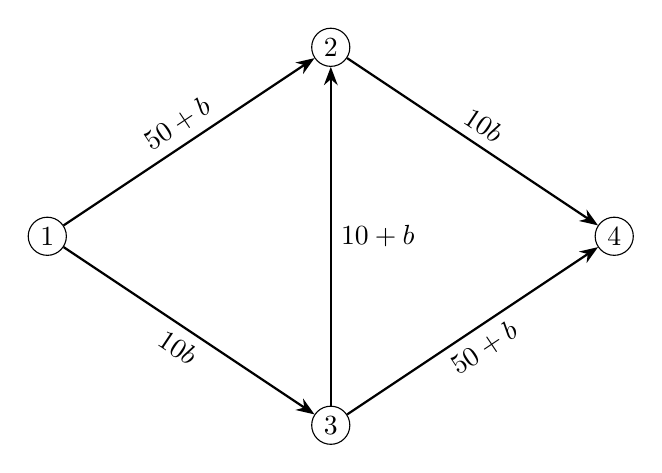
\begin{tikzpicture}[
        node distance=2cm and 3cm,
        main node/.style={circle, draw, fill=white, inner sep=2pt},
        every edge/.style={draw, -Stealth, thick},
        every label/.style={font=\small},
        scale=1.2
      ]
      % Nodes
      \node[main node] (P1) at (0,0) {$1$};
      \node[main node] (P2) at (3,2) {$2$};
      \node[main node] (P3) at (3,-2) {$3$};
      \node[main node] (P4) at (6,0) {$4$};

      % Edges with labels
      \draw (P1) edge node[above, sloped] {$50+b$} (P2);
      \draw (P2) edge node[above, sloped] {$10b$} (P4);
      \draw (P1) edge node[below, sloped] {$10b$} (P3);
      \draw (P3) edge node[below, sloped] {$50+b$} (P4);
      \draw (P3) edge node[right] {$10+b$} (P2);
    \end{tikzpicture}
  \end{center}
  \onslide<+->
  \begin{itemize}[<+->]
    \item Assume a flow of 6 units (e.g., 6000 vehicles) must travel from $1$ to $4$
    \item Three paths exist: $B_1 = 124$, $B_2 = 1324$, $B_3 = 134$
  \end{itemize}
\end{frame}

\begin{frame}{Braess' Example: Cont'd}
  \begin{itemize}[<+->]
    \item Case 1: All Paths Open. Split the flow equally (2 units each):
    \onslide<+->
    \begin{gather*}
      b_{12} = 2, \; b_{24} = 4, \; b_{34} = 2, \;b_{13} = 4, \; b_{32} = 2\\
      d_{12} = 52, \; d_{24} = 40, \; d_{34} = 52, \; d_{13} = 40, \; d_{32} = 12 \\
      L(B_1) = L(B_2) = L(B_3) = 92
    \end{gather*}
    \onslide<+->
    All paths are critical (maximal length). This distribution is stable: Switching paths increases load and travel time beyond 92.

    \item Case 2: Ban Edge $k_{32}$. Split flow equally between $B_1$ and $B_3$ (3 units each):
    \onslide<+->
    \begin{gather*}
      b_{12} = b_{24} = b_{13} = b_{34} = 3\\
      d_{12} = 53, \; d_{24} = 30, \; d_{13} = 30, \; d_{34} = 53\\
      L(B_1) = L(B_3) = 83
    \end{gather*}
    \onslide<+->
    Despite losing a connection, all paths are shorter!
\end{itemize}
\end{frame}

\begin{frame}{Braess' Example: Selfish Deviation}

  \begin{center}
    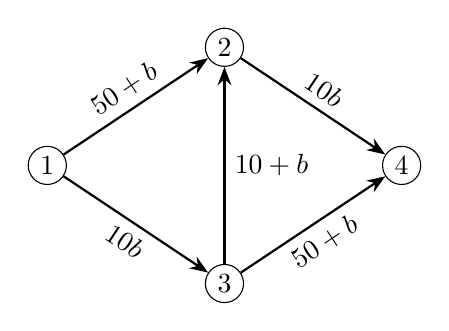
\begin{tikzpicture}[
        node distance=2cm and 3cm,
        main node/.style={circle, draw, fill=white, inner sep=2pt},
        every edge/.style={draw, -Stealth, thick},
        every label/.style={font=\small},
        scale=0.75
      ]
      % Nodes
      \node[main node] (P1) at (0,0) {$1$};
      \node[main node] (P2) at (3,2) {$2$};
      \node[main node] (P3) at (3,-2) {$3$};
      \node[main node] (P4) at (6,0) {$4$};

      % Edges with labels
      \draw (P1) edge node[above, sloped] {$50+b$} (P2);
      \draw (P2) edge node[above, sloped] {$10b$} (P4);
      \draw (P1) edge node[below, sloped] {$10b$} (P3);
      \draw (P3) edge node[below, sloped] {$50+b$} (P4);
      \draw (P3) edge node[right] {$10+b$} (P2);
    \end{tikzpicture}
  \end{center}
  \onslide<+->
  \begin{itemize}[<+->]
    \item Recall that $B_1 = 124$, $B_2 = 1324$, $B_3 = 134$
    \item A single vehicle ignoring the ban on $k_{32}$ (where $d_{32} = 10$) takes $B_2$ with $L(B_2) = 70$, gaining an advantage.
    \item If the ban is lifted, many use $B_2$, reverting to the original state. 
    \item Consider an intermediate step: 5 units on $B_1$ and $B_3$, 1 on $B_2$, then $L(B_1) = L(B_3) = 87.5$, $L(B_2) = 82.5$.
    \item $B_2$ users clog $k_{13}$ and $k_{24}$ (factor $10$ in load-time relation), worsening times for $B_1$ and $B_3$ beyond $83$; Yet $B_2$ remains shortest, attracting more traffic and degrading the system for all.
  \end{itemize}
\end{frame}

\begin{frame}{Real-Life Examples}
  \begin{itemize}[<+->]
    \item \href{https://www.youtube.com/watch?v=Cg73j3QYRJc}{The mechanical analogy: the spring paradox}
    \item \href{https://engines.egr.uh.edu/episode/2814}{Road closure in NY: Times and Herald Squares pedestrian plaza (2009 ---)}
      \begin{center}
        \includegraphics[scale=.3]{fig/note02/nybefore.png}\hspace{3mm}
        \includegraphics[scale=.3]{fig/note02/nyafter.png}
      \end{center}
      %\begin{itemize}
      %  \item Two sections of Broadway where it obliquely crosses major north/south boulevards at Times and Herald Squares 
      %  \item The experiment was successful and the road closures were made permanent
      %  \item Times and Herald Squares are now home to pedestrian plazas
      %\end{itemize}
    \item \href{https://en.wikipedia.org/wiki/Cheonggyecheon}{Cheonggyecheon restoration project (2003 ---)}
      \begin{itemize}
        \item Replaced a six lane highway with a five mile long park, traffic flow improved
      \end{itemize}
  \end{itemize}
\end{frame}


\section{References}

\begin{frame}[allowframebreaks]
  \frametitle{References}
  \nocite{*}
  \bibliographystyle{apalike}
  \bibliography{note02}
\end{frame}

\end{document}

\section{Voting Paradox}

\begin{frame}
  
  \begin{itemize}
    \item The Simplest Case
      \vspace{3mm}
      \begin{table}
        \center
        \begin{tabular}{cccc}
          \toprule
          \textbf{Voter} & \textbf{First preference} & \textbf{Second preference} & \textbf{Third preference} \\
          \midrule
          Voter 1 & A & B & C \\
          Voter 2 & B & C & A \\
          Voter 3 & C & A & B \\
          \bottomrule
        \end{tabular}
      \end{table}
      \vspace{3mm}
      \begin{center} A $>$ B $>$ C $>$ A \end{center}
      \vspace{1mm} 
    \item A More Complicated Situation
      \vspace{3mm}
      \begin{table}
        \center
        \begin{tabular}{llll}
          \toprule
          \textbf{Party} & \textbf{First preference} & \textbf{Second preference} & \textbf{Third preference} \\
          \midrule
          Left (3)   & education & health & security \\
          Center (4) & health & security & education \\
          Right (5)  & security & education & health \\
          \bottomrule
        \end{tabular}
      \end{table}
      \vspace{3mm}
        \begin{center} A $>$ B $>$ C $>$ A \end{center}
      \vspace{3mm} 
  \end{itemize}
\end{frame}

\section{Arrow's Impossibility Theorem}

\begin{frame}

\end{frame}

\section{St. Petersberg Paradox}

\begin{frame}{The Expected Utility Hypothesis}
\end{frame}

\begin{frame}{The Expected Utility Hypothesis}
  \begin{definition}
    The agent prefers the r.v. $X$ to r.v. $Y$ iff
    \begin{align*}
      \expc U(X) > \expc U(Y)
    \end{align*}
    where $\expc$ is the expectation operator, $U:\RR\mapsto\RR$ is the agent's utility function.
  \end{definition}
\end{frame}

\section{Allais Paradox}

\begin{frame}
  \begin{itemize}[<+->]\setlength\itemsep{0em}
    \item Game A
      \begin{align*}
        X = \begin{cases}101 & \text{prob. } 0.33\\100 & \text{prob. } 0.66\\ 0 & \text{prob. } 0.01 \end{cases} \qquad
        Y = 100 \;\text{ with prob. } 1
      \end{align*}
      \onslide<+->
      Mostly prefer $Y$ to $X$: from the Expected Utility Hypothesis 
      \onslide<+->
      \begin{multline}
        U(100) > 0.33\cdot U(101) + 0.66\cdot U(100) + 0.01\cdot U(0)\\ \ie 0.34\cdot U(100) > 0.33\cdot U(101) + 0.01\cdot U(0)
      \end{multline}
    \item Game B 
      \begin{align*}
        X = \begin{cases}100 & \text{prob. } 0.34\\ 0 & \text{prob. } 0.66 \end{cases} \qquad
        Y = \begin{cases}101 & \text{prob. } 0.33\\ 0 & \text{prob. } 0.67 \end{cases}
      \end{align*}
      \onslide<+->
      Mostly prefer $Y$ to $X$: from the Expected Utility Hypothesis 
      \onslide<+->
      \begin{multline}
        0.33\cdot U(101) + 0.67\cdot U(0) > 0.34\cdot U(100) + 0.66\cdot U(0)\\ \ie 0.33\cdot U(101) + 0.01\cdot U(0) > 0.34\cdot U(100)
      \end{multline}
  \end{itemize}
\end{frame}

\section{Ellsberg Paradox}

\begin{frame}
  \begin{itemize}[<+->]
    \item Given an urn with $30$ balls of colors red, yellow, and black
    \item There are $10$ red balls; total $20$ yellow / black balls, but the number of each type unknown
    \item The agent estimates the probability of drawing yellow as $p$ where $0 < p < \frac{2}{3}$
    \item A single ball is drawn from the urn
  \end{itemize}
\end{frame}

\begin{frame}
  \begin{itemize}[<+->]\setlength\itemsep{0em}
    \item Game A  
      \begin{align*}
        X = \begin{cases}100 & \text{if red}\\0 & \text{if yellow or black}\end{cases} \qquad
        Y = \begin{cases}100 & \text{if yellow}\\0 & \text{if red or black}\end{cases} \qquad
      \end{align*}
      \onslide<+->
      Mostly prefer $X$ to $Y$: from the Expected Utility Hypothesis 
      \onslide<+->
      \begin{multline}
        \frac{1}{3}\cdot U(100) + \frac{2}{3}\cdot U(0) > p\cdot U(100) + (1 - p)\cdot U(0) \\ \ie\big(\frac{1}{3} - p\big)\cdot U(100) > \big(\frac{1}{3} - p\big)\cdot U(0)
      \end{multline}
    \item Game B 
      \begin{align*}
        X = \begin{cases}100 & \text{if red or black}\\ 0 & \text{if yellow}\end{cases} \qquad
        Y = \begin{cases}100 & \text{if yellow or black}\\ 0 & \text{if red}\end{cases}
      \end{align*}
      \onslide<+->
      Mostly prefer $Y$ to $X$: from the Expected Utility Hypothesis 
      \onslide<+->
      \begin{multline}
        \frac{2}{3}\cdot U(100) + \frac{1}{3}\cdot U(0) > (1 - p)\cdot U(100) + p\cdot U(0) \\ \ie\big(\frac{1}{3} - p\big)\cdot U(0) > \big(\frac{1}{3} - p\big)\cdot U(100)
      \end{multline}
  \end{itemize}
\end{frame}

\end{document}
